% Anonymous ICLR 2027 manuscript. Build with ./build.sh. Numerical tables are generated.
\documentclass{article}
\usepackage{iclr2027_conference,times}

\usepackage[utf8]{inputenc}
\usepackage[T1]{fontenc}
\usepackage{amsmath,amssymb,amsfonts}
\usepackage{graphicx}
\usepackage{wrapfig}
\usepackage{booktabs}
\usepackage{multirow}
\usepackage{array}
\usepackage{xcolor}
\usepackage{tikz}
\usetikzlibrary{positioning,arrows.meta,calc,fit,backgrounds,shapes.geometric}
\usepackage{caption}
\captionsetup{font=small,labelfont=bf}
\usepackage{hyperref}
\hypersetup{hidelinks}
\usepackage{url}
\usepackage{microtype}
\usepackage{placeins}
\usepackage{float}
\usepackage{enumitem}
\setlist{nosep,leftmargin=*}

\usepackage{todonotes}
\usepackage{soul}

\graphicspath{{figures/}}
%
% macros.tex -- notation for the NM-ROM methods section.
% Symbol conventions (kept deliberately disjoint from the old submission, which
% overloaded K for both the discrete operator and a latent-adjacent quantity):
%   N  unknowns of the full-order state      k  latent dimension
%   R  spatial bank width (R' used by a query)   M  number of tests
%   N_eq  number of empirical-quadrature nodes

\newcommand{\Real}{\mathbb{R}}
\newcommand{\Nat}{\mathbb{N}}

% --- discrete objects -------------------------------------------------------
\newcommand{\Aop}{K}                    % fixed linear discrete operator
\newcommand{\bank}{G}                   % frozen spatial bank, n x R
\newcommand{\head}{h}            % nonlinear coefficient map, R^k -> R^R
\newcommand{\tests}{P}                  % weak test matrix, M x n
\newcommand{\rowscale}{\Lambda}         % diagonal row scaling
\newcommand{\lift}{u_{g}}               % boundary lift
\newcommand{\bcmask}{\mu}               % boundary mask / vanishing factor
\newcommand{\latent}{z}
\newcommand{\umanifold}{u}

% --- operators and norms ----------------------------------------------------
\newcommand{\jac}[1]{J_{#1}}
\newcommand{\dhead}{J_{h}}
\newcommand{\norm}[1]{\lVert #1 \rVert}
\newcommand{\normF}[1]{\lVert #1 \rVert_{F}}
\newcommand{\inner}[2]{\langle #1, #2 \rangle}
\newcommand{\T}{^{\top}}
\newcommand{\Tr}{\operatorname{tr}}
\newcommand{\diag}{\operatorname{diag}}
\newcommand{\rank}{\operatorname{rank}}
\newcommand{\argmin}{\operatorname*{arg\,min}}

% --- residuals --------------------------------------------------------------
\newcommand{\rfull}{R}                  % full discrete residual
\newcommand{\rweak}{r_{w}}              % weak (projected, row-scaled) residual
\newcommand{\station}[2]{\eta(#1,#2)}   % normalized-gradient stationarity measure

% --- placeholders for generated numbers -------------------------------------
% Every numeric value in this manuscript must come from a generator script that
% reads the run JSONs. \todo marks a slot that the generator has not yet filled.
% \todo now comes from todonotes (line 22); the local definition clashed with it.
\newcommand{\gen}[1]{\todo{pending: #1}}

% Subscripted variants (the base macros already carry a subscript, so
% \head_a / \rweak_n would be a double subscript).
\newcommand{\headc}[1]{h_{#1}}   % one component of the head output
\newcommand{\rweakn}[1]{r_{w,#1}}       % the weak residual of time step #1

%
% GENERATED by paper/gen_tables.py -- do not edit.
% Every prose number in the manuscript is one of these macros.
\newcommand{\nAblBurgersBestFound}{2.5447}
\newcommand{\nAblBurgersFloor}{0.3918}
\newcommand{\nAblBurgersFree}{0.6027}
\newcommand{\nAblBurgersFreeMs}{2417.6}
\newcommand{\nAblBurgersLinear}{56.9296}
\newcommand{\nAblBurgersNeural}{2.5629}
\newcommand{\nAblBurgersNeuralMs}{47.6}
\newcommand{\nAblBurgersPodOneTwentyEight}{10.1198}
\newcommand{\nAblBurgersPodOneTwentyEightMs}{328.3}
\newcommand{\nAblBurgersPodSixteen}{61.6503}
\newcommand{\nAblBurgersQuad}{31.8276}
\newcommand{\nAblBurgersReductionOverFloor}{6.5}
\newcommand{\nAblBurgersSolverGapPp}{0.018}
\newcommand{\nAblPoissonBestFound}{6.0926}
\newcommand{\nAblPoissonDst}{0.0007}
\newcommand{\nAblPoissonDstMs}{4.341}
\newcommand{\nAblPoissonFloor}{2.3148}
\newcommand{\nAblPoissonFree}{2.3274}
\newcommand{\nAblPoissonLinear}{17.2966}
\newcommand{\nAblPoissonNeural}{6.0927}
\newcommand{\nAblPoissonNeuralMs}{5.843}
\newcommand{\nAblPoissonPodOneTwentyEight}{4.3452}
\newcommand{\nAblPoissonPodOneTwentyEightMs}{5.930}
\newcommand{\nAblPoissonPodSixteen}{20.0548}
\newcommand{\nAblPoissonQthirtytwo}{4.6670}
\newcommand{\nAblPoissonQthirtytwoMs}{7.317}
\newcommand{\nAblPoissonQuad}{16.6303}
\newcommand{\nBlockBlockBudgetExits}{0}
\newcommand{\nBlockBlockErr}{2.1489}
\newcommand{\nBlockBlockMs}{619.2}
\newcommand{\nBlockJointBudgetExits}{6}
\newcommand{\nBlockJointErr}{2.1489}
\newcommand{\nBlockJointMs}{1119.7}
\newcommand{\nCgLshapeCgTol}{$10^{-10}$}
\newcommand{\nCgLshapeMeshes}{$64^2$, $128^2$, $256^2$, $512^2$}
\newcommand{\nCgLshapePcgRatioMax}{990.8}
\newcommand{\nCgLshapePcgRatioMin}{3.6}
\newcommand{\nCgLshapeSpeedupMax}{14.9}
\newcommand{\nCgLshapeSpeedupMin}{2.9}
\newcommand{\nCgPoissonCgMsTwoFiftySix}{38.0}
\newcommand{\nCgPoissonDstFasterMax}{4.0}
\newcommand{\nCgPoissonDstFasterMin}{1.3}
\newcommand{\nCgPoissonSpeedupMax}{23.4}
\newcommand{\nCgPoissonSpeedupMin}{3.7}
\newcommand{\nColdCapEightNearest}{6.09}
\newcommand{\nColdCapEightZero}{30.03}
\newcommand{\nColdCapTwelveNearest}{6.09}
\newcommand{\nColdCapTwelveZero}{6.09}
\newcommand{\nColdCapTwoNearest}{6.80}
\newcommand{\nColdCapTwoZero}{91.88}
\newcommand{\nColdConvNearest}{6.09}
\newcommand{\nColdConvZero}{6.09}
\newcommand{\nColdMesh}{1024}
\newcommand{\nColdStarts}{nearest, zero}
\newcommand{\nEqtopBar}{0.116}
\newcommand{\nEqtopBarOrigin}{the held-out $\rho$ of the incumbent $q{=}0$ rule at the state carrying the first-interval penalty, measured in the q-diag cell and adopted as the primary bar in the q-ridge design before any certification job ran; the tight bar was declared before b-eqtop ran}
\newcommand{\nEqtopConfirmedCount}{3}
\newcommand{\nEqtopConfirmedRungs}{0, 16, 32}
\newcommand{\nEqtopCostRatioMax}{0.21}
\newcommand{\nEqtopCostRatioMin}{0.18}
\newcommand{\nEqtopLadderConverged}{yes}
\newcommand{\nEqtopLadderCostSpan}{12.23}
\newcommand{\nEqtopLadderErrSpan}{3.51}
\newcommand{\nEqtopLadderFirstErr}{1.8891}
\newcommand{\nEqtopLadderFirstMs}{59.1}
\newcommand{\nEqtopLadderLastErr}{0.5389}
\newcommand{\nEqtopLadderLastMs}{722.2}
\newcommand{\nEqtopLadderMonotone}{yes}
\newcommand{\nEqtopMarginalCount}{3}
\newcommand{\nEqtopMarginalRungs}{64 (2/6), 128 (4/5), 256 (1/5)}
\newcommand{\nEqtopParentOneTwentyEightRho}{0.1908}
\newcommand{\nEqtopParentTwoFiftySixRho}{0.1678}
\newcommand{\nEqtopPendingJob}{none}
\newcommand{\nEqtopPrimaryOneTwentyEight}{yes}
\newcommand{\nEqtopPrimaryOneTwentyEightM}{2048}
\newcommand{\nEqtopPrimaryOneTwentyEightRho}{0.0669}
\newcommand{\nEqtopPrimaryOneTwentyEightStates}{64}
\newcommand{\nEqtopPrimaryTwoFiftySix}{yes}
\newcommand{\nEqtopPrimaryTwoFiftySixM}{2048}
\newcommand{\nEqtopPrimaryTwoFiftySixRho}{0.1074}
\newcommand{\nEqtopPrimaryTwoFiftySixStates}{64}
\newcommand{\nEqtopQsixtyFourArchivedRho}{0.0531}
\newcommand{\nEqtopQsixtyFourRedrawRho}{0.1220}
\newcommand{\nEqtopSpreadMax}{9.6}
\newcommand{\nEqtopSpreadMin}{1.4}
\newcommand{\nEqtopStaticWorstFit}{1.5e-04}
\newcommand{\nEqtopStaticWorstOverBar}{4.0}
\newcommand{\nEqtopStaticWorstQ}{256}
\newcommand{\nEqtopStaticWorstRho}{0.462}
\newcommand{\nEqtopStatus}{final}
\newcommand{\nEqtopStatusQOneTwentyEight}{marginal (4 of 5 draws pass)}
\newcommand{\nEqtopStatusQSixteen}{confirmed (3 of 3 re-draws)}
\newcommand{\nEqtopStatusQSixtyFour}{marginal (2 of 6 draws pass)}
\newcommand{\nEqtopStatusQThirtyTwo}{confirmed (2 of 2 re-draws)}
\newcommand{\nEqtopStatusQTwoFiftySix}{marginal (1 of 5 draws pass)}
\newcommand{\nEqtopStatusQZero}{confirmed (3 of 3 re-draws)}
\newcommand{\nEqtopTightBar}{0.06}
\newcommand{\nEqtopTopDenseErr}{0.5194}
\newcommand{\nEqtopTopDenseMs}{3915.1}
\newcommand{\nEqtopTopDraws}{1 of 5}
\newcommand{\nEqtopTopEqErr}{0.5389}
\newcommand{\nEqtopTopEqMs}{722.2}
\newcommand{\nEqtopTopM}{2048}
\newcommand{\nEqtopTopOldRuleErr}{1.0361}
\newcommand{\nEqtopTopOldRuleRho}{0.1678}
\newcommand{\nEqtopTopRedrawMin}{0.182}
\newcommand{\nEqtopTopRedrawRange}{0.130--0.242}
\newcommand{\nEqtopTopRho}{0.1074}
\newcommand{\nHeatBankErrTenTwentyFour}{1.68}
\newcommand{\nHeatBankErrTwoFiftySix}{1.68}
\newcommand{\nHeatBankMsTenTwentyFour}{0.56}
\newcommand{\nHeatBankMsTwoFiftySix}{0.14}
\newcommand{\nHeatBankOverHeadCostTenTwentyFour}{22}
\newcommand{\nHeatBankOverHeadCostTwoFiftySix}{86}
\newcommand{\nHeatFomMsTenTwentyFour}{1.03}
\newcommand{\nHeatFomMsTwoFiftySix}{0.21}
\newcommand{\nHeatHeadErrTenTwentyFour}{4.56}
\newcommand{\nHeatHeadErrTwoFiftySix}{4.56}
\newcommand{\nHeatHeadMsTenTwentyFour}{12.3}
\newcommand{\nHeatHeadMsTwoFiftySix}{11.9}
\newcommand{\nLinearBankOverPodMax}{4.0}
\newcommand{\nLinearBankOverPodMin}{3.4}
\newcommand{\nLshapeBestFloor}{0.6650}
\newcommand{\nLshapeBestFloorCommon}{1.6155}
\newcommand{\nLshapeCheapestFomErrFiveTwelve}{0.385}
\newcommand{\nLshapeCheapestFomErrOneTwentyEight}{0.000}
\newcommand{\nLshapeCheapestFomErrSixtyFour}{0.000}
\newcommand{\nLshapeCheapestFomErrTwoFiftySix}{0.000}
\newcommand{\nLshapeCheapestFomFiveTwelve}{CG $10^{-2}$}
\newcommand{\nLshapeCheapestFomMoreAccurateFiveTwelve}{5.5}
\newcommand{\nLshapeCheapestFomMoreAccurateOneTwentyEight}{exact}
\newcommand{\nLshapeCheapestFomMoreAccurateSixtyFour}{exact}
\newcommand{\nLshapeCheapestFomMoreAccurateTwoFiftySix}{exact}
\newcommand{\nLshapeCheapestFomMsFiveTwelve}{29.13}
\newcommand{\nLshapeCheapestFomMsOneTwentyEight}{2.48}
\newcommand{\nLshapeCheapestFomMsSixtyFour}{1.28}
\newcommand{\nLshapeCheapestFomMsTwoFiftySix}{8.39}
\newcommand{\nLshapeCheapestFomOneTwentyEight}{sparse direct (SuperLU)}
\newcommand{\nLshapeCheapestFomSixtyFour}{sparse direct (SuperLU)}
\newcommand{\nLshapeCheapestFomTwoFiftySix}{sparse direct (SuperLU)}
\newcommand{\nLshapeDevelopmentWorst}{6.8}
\newcommand{\nLshapeEnrichFloor}{0.6650}
\newcommand{\nLshapeEnrichGain}{1.067}
\newcommand{\nLshapeFiveTwelveBestPod}{POD $k'{=}128$}
\newcommand{\nLshapeFiveTwelveBestPodErr}{2.451}
\newcommand{\nLshapeFiveTwelveBestPodMs}{4.031}
\newcommand{\nLshapeFiveTwelveBestReduced}{head $q{=}64$ (head\_sdf\_R512\_K16)}
\newcommand{\nLshapeFiveTwelveBestReducedErr}{2.123}
\newcommand{\nLshapeFiveTwelveCgErr}{0.385}
\newcommand{\nLshapeFiveTwelveCgMs}{29.13}
\newcommand{\nLshapeFreeErr}{0.7791}
\newcommand{\nLshapeFreeFaster}{1.54}
\newcommand{\nLshapeFreeMoreAccurate}{1.19}
\newcommand{\nLshapeFreeMs}{2.583}
\newcommand{\nLshapeFreeOverFloor}{1.003}
\newcommand{\nLshapeHeadIndepBitwise}{no}
\newcommand{\nLshapeHeadIndepRel}{4.06e-14}
\newcommand{\nLshapeHeadOverPodCostFiveTwelve}{19}
\newcommand{\nLshapeHeadOverPodCostOneTwentyEight}{2}
\newcommand{\nLshapeHeadOverPodCostSixtyFour}{5}
\newcommand{\nLshapeHeadOverPodCostTwoFiftySix}{6}
\newcommand{\nLshapeHeadRatioMax}{5.77}
\newcommand{\nLshapeHeadRatioMin}{2.24}
\newcommand{\nLshapeJobCount}{5}
\newcommand{\nLshapeKsixteenBest}{3.8607}
\newcommand{\nLshapeKthirtytwoBest}{3.1802}
\newcommand{\nLshapeNeuralCheaper}{2.77}
\newcommand{\nLshapeNeuralCheaperFiveTwelve}{7.60}
\newcommand{\nLshapeNeuralCheaperOneTwentyEight}{0.88}
\newcommand{\nLshapeNeuralCheaperSixtyFour}{0.45}
\newcommand{\nLshapeNeuralCheaperTwoFiftySix}{2.77}
\newcommand{\nLshapeNeuralCheaperVsCheapestFiveTwelve}{6.07}
\newcommand{\nLshapeNeuralCheaperVsCheapestOneTwentyEight}{0.88}
\newcommand{\nLshapeNeuralCheaperVsCheapestSixtyFour}{0.45}
\newcommand{\nLshapeNeuralCheaperVsCheapestTwoFiftySix}{2.77}
\newcommand{\nLshapeNeuralErr}{2.131}
\newcommand{\nLshapeNeuralErrFiveTwelve}{2.123}
\newcommand{\nLshapeNeuralErrOneTwentyEight}{2.164}
\newcommand{\nLshapeNeuralErrSixtyFour}{2.300}
\newcommand{\nLshapeNeuralErrTwoFiftySix}{2.131}
\newcommand{\nLshapeNeuralMs}{3.028}
\newcommand{\nLshapeNeuralMsFiveTwelve}{4.801}
\newcommand{\nLshapeNeuralMsOneTwentyEight}{2.806}
\newcommand{\nLshapeNeuralMsSixtyFour}{2.846}
\newcommand{\nLshapeNeuralMsTrend}{2.85 $\to$ 2.81 $\to$ 3.03 $\to$ 4.80}
\newcommand{\nLshapeNeuralMsTwoFiftySix}{3.028}
\newcommand{\nLshapeNeuralNonDomFiveTwelve}{yes}
\newcommand{\nLshapeNeuralNonDomOneTwentyEight}{no}
\newcommand{\nLshapeNeuralNonDomSixtyFour}{no}
\newcommand{\nLshapeNeuralNonDomTwoFiftySix}{yes}
\newcommand{\nLshapeNonDomCount}{7}
\newcommand{\nLshapeNonDomCountFiveTwelve}{8}
\newcommand{\nLshapeNonDomCountOneTwentyEight}{4}
\newcommand{\nLshapeNonDomCountSixtyFour}{1}
\newcommand{\nLshapeNonDomCountTwoFiftySix}{7}
\newcommand{\nLshapeNonDomReduced}{6}
\newcommand{\nLshapeNonDomReducedFiveTwelve}{6}
\newcommand{\nLshapeNonDomReducedOneTwentyEight}{3}
\newcommand{\nLshapeNonDomReducedSixtyFour}{0}
\newcommand{\nLshapeNonDomReducedTwoFiftySix}{6}
\newcommand{\nLshapeOneTwentyEightBestReduced}{POD $k'{=}64$}
\newcommand{\nLshapeOneTwentyEightBestReducedCheaper}{1.08}
\newcommand{\nLshapeOneTwentyEightBestReducedErr}{7.701}
\newcommand{\nLshapeOneTwentyEightCheapRange}{1.08--1.19}
\newcommand{\nLshapeOneTwentyEightReducedErrRange}{7.7--34.6}
\newcommand{\nLshapePodCheaperFiveTwelve}{9.06}
\newcommand{\nLshapePodCheaperOneTwentyEight}{0.90}
\newcommand{\nLshapePodCheaperSixtyFour}{0.47}
\newcommand{\nLshapePodCheaperTwoFiftySix}{2.94}
\newcommand{\nLshapePodCheaperVsCheapestFiveTwelve}{7.23}
\newcommand{\nLshapePodCheaperVsCheapestOneTwentyEight}{0.90}
\newcommand{\nLshapePodCheaperVsCheapestSixtyFour}{0.47}
\newcommand{\nLshapePodCheaperVsCheapestTwoFiftySix}{2.94}
\newcommand{\nLshapePodErrFiveTwelve}{2.451}
\newcommand{\nLshapePodErrOneTwentyEight}{2.483}
\newcommand{\nLshapePodErrSixtyFour}{2.591}
\newcommand{\nLshapePodErrTwoFiftySix}{2.457}
\newcommand{\nLshapePodMsFiveTwelve}{4.031}
\newcommand{\nLshapePodMsOneTwentyEight}{2.764}
\newcommand{\nLshapePodMsSixtyFour}{2.711}
\newcommand{\nLshapePodMsTwoFiftySix}{2.850}
\newcommand{\nLshapePodOverHeadErrFiveTwelve}{15}
\newcommand{\nLshapePodOverHeadErrOneTwentyEight}{15}
\newcommand{\nLshapePodOverHeadErrSixtyFour}{13}
\newcommand{\nLshapePodOverHeadErrTwoFiftySix}{15}
\newcommand{\nLshapePodTwoFiftySixErr}{0.9303}
\newcommand{\nLshapePodTwoFiftySixMs}{3.987}
\newcommand{\nLshapeSdfFloor}{0.7698}
\newcommand{\nLshapeSelectedFloorCommon}{1.6155}
\newcommand{\nLshapeSmoothFloor}{0.7093}
\newcommand{\nLshapeSolve}{in Table~\ref{tab:lshape-solve} ($64^2$--$512^2$, one job per mesh)}
\newcommand{\nLshapeSpluMsFiveTwelve}{36.50}
\newcommand{\nLshapeSpluMsOneTwentyEight}{2.48}
\newcommand{\nLshapeSpluMsSixtyFour}{1.28}
\newcommand{\nLshapeSpluMsTwoFiftySix}{8.39}
\newcommand{\nLshapeValidationGap}{2.5}
\newcommand{\nLshapeValidationWorst}{16.7}
\newcommand{\nLvAllConverged}{yes}
\newcommand{\nLvAnyNeuralNonDom}{no}
\newcommand{\nLvAnyReducedNonDom}{no}
\newcommand{\nLvBankFloorCollapse}{19.00$\times$}
\newcommand{\nLvBankFloorInc}{0.3918}
\newcommand{\nLvBankFloorLow}{7.4455}
\newcommand{\nLvBestFoundInc}{2.5447}
\newcommand{\nLvBestFoundLow}{11.3934}
\newcommand{\nLvBestFoundRatio}{4.48$\times$}
\newcommand{\nLvBudgetExitsTotal}{0}
\newcommand{\nLvCheapestDominatingFom}{\texttt{nt1e-2\_dt01}}
\newcommand{\nLvCheapestDominatingFomErr}{3.90}
\newcommand{\nLvCheapestDominatingFomMs}{14.0}
\newcommand{\nLvControlMonotone}{no}
\newcommand{\nLvDiscMax}{20.9}
\newcommand{\nLvDiscMin}{19.3}
\newcommand{\nLvDiscTight}{20.8}
\newcommand{\nLvFfourDiscRatio}{5.17}
\newcommand{\nLvFreeBank}{7.7940}
\newcommand{\nLvFreeBankMs}{3174.6}
\newcommand{\nLvFtwoFires}{no}
\newcommand{\nLvLadderConverged}{yes}
\newcommand{\nLvLadderCostSpan}{3.25$\times$}
\newcommand{\nLvLadderErrSpan}{1.36$\times$}
\newcommand{\nLvLadderKnobBar}{no}
\newcommand{\nLvLadderMonotone}{yes}
\newcommand{\nLvLadderQtop}{6.6718}
\newcommand{\nLvLadderQtopMs}{1810.3}
\newcommand{\nLvLadderQzero}{9.0500}
\newcommand{\nLvLadderQzeroMs}{557.4}
\newcommand{\nLvLadderRefMax}{19.44}
\newcommand{\nLvLadderRefMin}{17.98}
\newcommand{\nLvLinearBestReduced}{7.7940}
\newcommand{\nLvLinearCollapseMax}{19}
\newcommand{\nLvLinearCollapseMin}{12}
\newcommand{\nLvMostAccurateReduced}{\texttt{q256\_M2176\_dense\_g1em06}}
\newcommand{\nLvMostAccurateReducedErr}{6.1869}
\newcommand{\nLvMostAccurateReducedMs}{2864.2}
\newcommand{\nLvNeuralBeatsLinearFromQ}{128}
\newcommand{\nLvNeuralBeatsPodFromQ}{0}
\newcommand{\nLvNeuralDegradeMax}{4.5}
\newcommand{\nLvNeuralDegradeMin}{3.3}
\newcommand{\nLvNonDomCount}{4}
\newcommand{\nLvNonDomList}{\texttt{nt1e-2\_dt01}, \texttt{nt1e-3\_dt005}, \texttt{dense\_tight}, \texttt{fft\_tight}}
\newcommand{\nLvPodBestReduced}{11.2540}
\newcommand{\nLvPodFiveTwelveCollapse}{12.09$\times$}
\newcommand{\nLvPodFiveTwelveFloor}{5.61}
\newcommand{\nLvPodMax}{57.9837}
\newcommand{\nLvPodMin}{11.2540}
\newcommand{\nLvPodMonotone}{no}
\newcommand{\nLvReducedOnlyNeuralMinQ}{64}
\newcommand{\nLvReducedOnlyNeuralQs}{64, 128, 256}
\newcommand{\nLvSolvedInc}{2.5629}
\newcommand{\nLvSolvedLow}{8.3933}
\newcommand{\nLvSolvedOverBestFound}{0.74}
\newcommand{\nLvSolvedRatio}{3.27$\times$}
\newcommand{\nLvSubjects}{27}
\newcommand{\nMeshBurgersCachedFirst}{44.16}
\newcommand{\nMeshBurgersCachedLast}{43.58}
\newcommand{\nMeshBurgersCachedRatio}{0.987}
\newcommand{\nMeshBurgersCompleteRatio}{1.52}
\newcommand{\nMeshBurgersDeviceRatio}{1.033}
\newcommand{\nMeshBurgersErrFirst}{10.8570}
\newcommand{\nMeshBurgersErrLast}{3.8847}
\newcommand{\nMeshBurgersEverFaster}{no}
\newcommand{\nMeshBurgersFomOverRomRange}{0.265--0.495}
\newcommand{\nMeshBurgersUnknownGrowth}{264}
\newcommand{\nMeshPoissonCachedFirst}{2.09}
\newcommand{\nMeshPoissonCachedLast}{2.02}
\newcommand{\nMeshPoissonCachedRatio}{0.965}
\newcommand{\nMeshPoissonCompleteRatio}{2.05}
\newcommand{\nMeshPoissonDeviceRatio}{1.334}
\newcommand{\nMeshPoissonErrFirst}{6.1119}
\newcommand{\nMeshPoissonErrLast}{6.1106}
\newcommand{\nMeshPoissonEverFaster}{no}
\newcommand{\nMeshPoissonFomOverRomRange}{0.063--0.112}
\newcommand{\nMeshPoissonUnknownGrowth}{264}
\newcommand{\nNsBankFloorMedian}{1.2242}
\newcommand{\nNsBankMedian}{3.6664}
\newcommand{\nNsBankOverPod}{1.08}
\newcommand{\nNsBankRank}{256}
\newcommand{\nNsBankWorst}{14.0838}
\newcommand{\nNsBudgetExitsKsixteen}{12}
\newcommand{\nNsBudgetExitsKthirtyTwo}{18}
\newcommand{\nNsCellArms}{4}
\newcommand{\nNsCellRatioMax}{1.46}
\newcommand{\nNsCellRatioMin}{1.15}
\newcommand{\nNsDataBankMedian}{3.7513}
\newcommand{\nNsDataBankOverPod}{1.20}
\newcommand{\nNsDataBankWorst}{13.8371}
\newcommand{\nNsDataBaseGap}{4.0}
\newcommand{\nNsDataBaseTrainRecon}{5.0345}
\newcommand{\nNsDataBudgetExits}{6}
\newcommand{\nNsDataFactor}{4}
\newcommand{\nNsDataHeldoutOverTrain}{1.3}
\newcommand{\nNsDataOracleMedian}{16.6598}
\newcommand{\nNsDataOraclePass}{no}
\newcommand{\nNsDataOracleRatio}{1.46}
\newcommand{\nNsDataPodMedian}{24.2492}
\newcommand{\nNsDataPodOverOracleEvolved}{1.39}
\newcommand{\nNsDataPodOverOracleTzero}{0.52}
\newcommand{\nNsDataPodTwoFiftySixWorst}{11.5733}
\newcommand{\nNsDataTrainBase}{512}
\newcommand{\nNsDataTrainExtra}{1536}
\newcommand{\nNsDataTrainN}{2048}
\newcommand{\nNsDataTrainRecon}{12.3875}
\newcommand{\nNsExpBankFloor}{1.7434}
\newcommand{\nNsExpBudgetExitsTotal}{0}
\newcommand{\nNsExpCases}{8}
\newcommand{\nNsExpCostRatio}{3.9}
\newcommand{\nNsExpEnergyList}{26, 44, 68, 92, 100}
\newcommand{\nNsExpEnergyRule}{field-metric POD of eta - h(z*), z* best-found by multi-start LM; nested in q}
\newcommand{\nNsExpEnstrophyMidMax}{0.97}
\newcommand{\nNsExpEnstrophyMidMin}{0.95}
\newcommand{\nNsExpEnstrophyPodThirtyTwo}{1.026}
\newcommand{\nNsExpEnstrophyQthirtyTwo}{0.990}
\newcommand{\nNsExpEnstrophyQtop}{0.999}
\newcommand{\nNsExpEnstrophyQzero}{1.043}
\newcommand{\nNsExpFomLooseMs}{421.3}
\newcommand{\nNsExpFomLooseWorst}{0.0041}
\newcommand{\nNsExpFomRefMs}{1177.7}
\newcommand{\nNsExpGain}{11.4}
\newcommand{\nNsExpK}{32}
\newcommand{\nNsExpM}{2176}
\newcommand{\nNsExpManifoldQzero}{16.4787}
\newcommand{\nNsExpManifoldTop}{1.7434}
\newcommand{\nNsExpMonotoneMedian}{yes}
\newcommand{\nNsExpMonotoneWorst}{no}
\newcommand{\nNsExpNonDomList}{\texttt{fom\_ntol0.0001}, \texttt{fom\_ntol0.001}, \texttt{fom\_ntol0.003}, \texttt{fom\_ntol0.03}, \texttt{fom\_ntol1e-06}, \texttt{fom\_ntol1e-11}, \texttt{pod\_k32}}
\newcommand{\nNsExpNonDomNeuralCount}{0}
\newcommand{\nNsExpPerTimeAccumulates}{yes}
\newcommand{\nNsExpPodBetterEveryRung}{no}
\newcommand{\nNsExpPodCheaperCount}{5}
\newcommand{\nNsExpPodCheaperMaxQ}{256}
\newcommand{\nNsExpPodMoreAccurateEveryRung}{yes}
\newcommand{\nNsExpQList}{32, 64, 128, 256, 512}
\newcommand{\nNsExpQtop}{512}
\newcommand{\nNsExpQzeroMedian}{41.3922}
\newcommand{\nNsExpQzeroWorst}{68.7654}
\newcommand{\nNsExpR}{512}
\newcommand{\nNsExpReps}{3}
\newcommand{\nNsExpRungCount}{6}
\newcommand{\nNsExpSolveOverManifoldDecreasing}{yes}
\newcommand{\nNsExpSolveOverManifoldMax}{2.5}
\newcommand{\nNsExpSolveOverManifoldMedFortyEightMax}{10.8}
\newcommand{\nNsExpSolveOverManifoldMedFortyEightMin}{2.9}
\newcommand{\nNsExpSolveOverManifoldMin}{1.4}
\newcommand{\nNsExpSolveOverManifoldPerTimeFirst}{1.44}
\newcommand{\nNsExpSolveOverManifoldPerTimeLast}{3.85}
\newcommand{\nNsExpSolveOverManifoldPerTimeList}{1.44, 1.66, 2.19, 2.89, 3.85}
\newcommand{\nNsExpSolveOverManifoldQtop}{1.40}
\newcommand{\nNsExpSolveOverManifoldQzero}{2.51}
\newcommand{\nNsExpTopMedian}{2.4377}
\newcommand{\nNsExpTopWorst}{6.0140}
\newcommand{\nNsFamBankFloorMedian}{0.2774}
\newcommand{\nNsFamBankMedian}{1.0820}
\newcommand{\nNsFamBankOverPod}{1.03}
\newcommand{\nNsFamBankWorst}{6.4018}
\newcommand{\nNsFamBaseGap}{4.0}
\newcommand{\nNsFamBaseOracleRatio}{1.19}
\newcommand{\nNsFamBudgetExits}{4}
\newcommand{\nNsFamDimBase}{14}
\newcommand{\nNsFamDimLow}{8}
\newcommand{\nNsFamDropFloor}{4.4}
\newcommand{\nNsFamDropMax}{4.4}
\newcommand{\nNsFamDropMin}{3.3}
\newcommand{\nNsFamDropOracle}{3.8}
\newcommand{\nNsFamDropPod}{3.3}
\newcommand{\nNsFamHeldoutOverTrain}{3.8}
\newcommand{\nNsFamLowModes}{3}
\newcommand{\nNsFamLowTrainN}{512}
\newcommand{\nNsFamOracleMedian}{5.2823}
\newcommand{\nNsFamOraclePass}{no}
\newcommand{\nNsFamOracleRatio}{1.39}
\newcommand{\nNsFamPodMedian}{7.3651}
\newcommand{\nNsFamPodOverOracleEvolved}{1.44}
\newcommand{\nNsFamPodOverOracleTzero}{1.83}
\newcommand{\nNsFamPodTwoFiftySixWorst}{6.2295}
\newcommand{\nNsFamTrainRecon}{1.3853}
\newcommand{\nNsHeldoutOverTrain}{4.0}
\newcommand{\nNsKthirtyTwo}{landed (job 3787320): fails the same bar (Table~\ref{tab:ns})}
\newcommand{\nNsKthirtyTwoHeldoutOverTrain}{3.2}
\newcommand{\nNsKthirtyTwoOracleMedian}{12.0948}
\newcommand{\nNsKthirtyTwoOraclePass}{no}
\newcommand{\nNsKthirtyTwoOracleRatio}{1.15}
\newcommand{\nNsKthirtyTwoOracleRatioMax}{1.16}
\newcommand{\nNsKthirtyTwoOracleRatioMin}{1.15}
\newcommand{\nNsKthirtyTwoPodMedian}{13.9455}
\newcommand{\nNsKthirtyTwoPodOverOracleEvolved}{1.16}
\newcommand{\nNsKthirtyTwoPodOverOracleTzero}{0.82}
\newcommand{\nNsOracleBar}{2.0}
\newcommand{\nNsOracleChange}{-0.04}
\newcommand{\nNsOracleMedian}{20.2417}
\newcommand{\nNsOraclePass}{no}
\newcommand{\nNsOracleRatio}{1.19}
\newcommand{\nNsOracleTzero}{2.5811}
\newcommand{\nNsPodOverOracleEvolved}{1.19}
\newcommand{\nNsPodOverOracleTzero}{1.63}
\newcommand{\nNsPodSixteenMedian}{24.0219}
\newcommand{\nNsPodTwoFiftySixMedian}{3.2750}
\newcommand{\nNsPodTwoFiftySixWorst}{13.0322}
\newcommand{\nNsPodTzero}{4.1970}
\newcommand{\nNsPrevOracleMedian}{20.2801}
\newcommand{\nNsPrevRank}{128}
\newcommand{\nNsPrevTrainRecon}{20.5576}
\newcommand{\nNsRom}{confirmatory campaign not run; exploratory ladder in Table~\ref{tab:ns-ladder}}
\newcommand{\nNsScaleBandHi}{-0.10}
\newcommand{\nNsScaleBandLo}{-0.25}
\newcommand{\nNsScaleGainFirstDoubling}{25}
\newcommand{\nNsScaleGainFirstMax}{25}
\newcommand{\nNsScaleGainFirstMin}{13}
\newcommand{\nNsScaleGainSecondDoubling}{4}
\newcommand{\nNsScaleGainSecondMax}{8}
\newcommand{\nNsScaleGainSecondMin}{4}
\newcommand{\nNsScalePlainNFiveTwelve}{19.8279}
\newcommand{\nNsScalePlainNOneTwentyEight}{27.4938}
\newcommand{\nNsScalePlainNTwoFiftySix}{20.6889}
\newcommand{\nNsScalePlainSlope}{-0.236}
\newcommand{\nNsScalePlainVerdict}{ambiguous}
\newcommand{\nNsScaleRegMoveMaxPct}{2.2}
\newcommand{\nNsScaleRegMovePct}{2.2}
\newcommand{\nNsScaleRegNFiveTwelve}{19.3892}
\newcommand{\nNsScaleRegNOneTwentyEight}{26.1095}
\newcommand{\nNsScaleRegNTwoFiftySix}{21.0204}
\newcommand{\nNsScaleRegSlope}{-0.215}
\newcommand{\nNsScaleRegSmallMovePct}{1.3}
\newcommand{\nNsScaleRegSmallNFiveTwelve}{20.0874}
\newcommand{\nNsScaleRegSmallNOneTwentyEight}{24.6583}
\newcommand{\nNsScaleRegSmallNTwoFiftySix}{21.3431}
\newcommand{\nNsScaleRegSmallSlope}{-0.148}
\newcommand{\nNsScaleRegSmallVerdict}{ambiguous}
\newcommand{\nNsScaleRegVerdict}{ambiguous}
\newcommand{\nNsSingleOverOracle}{1.10}
\newcommand{\nNsSingleStartMedian}{22.3139}
\newcommand{\nNsTrainImprovement}{4.1}
\newcommand{\nNsTrainRecon}{5.0345}
\newcommand{\nOfflineDirectionSeconds}{1242}
\newcommand{\nOfflineFitHoursLadderTotal}{1.7}
\newcommand{\nOfflineFitSecondsLadderTotal}{6102}
\newcommand{\nOfflineFitSecondsQOneTwentyEight}{2920}
\newcommand{\nOfflineFitSecondsQSixteen}{147}
\newcommand{\nOfflineFitSecondsQSixtyFour}{160}
\newcommand{\nOfflineFitSecondsQThirtyTwo}{155}
\newcommand{\nOfflineFitSecondsQTwoFiftySix}{2650}
\newcommand{\nOfflineFitSecondsQZero}{72}
\newcommand{\nOfflineTrainSecondsBest}{1459}
\newcommand{\nOfflineTrainSecondsLikeForLike}{387}
\newcommand{\nOpAllImproving}{11 of 12}
\newcommand{\nOpArmsBeatingRom}{4}
\newcommand{\nOpCohortSize}{8}
\newcommand{\nOpCtrlCount}{3}
\newcommand{\nOpCtrlMediumFSixtyFour}{1.6721}
\newcommand{\nOpCtrlMediumFSixtyFourEpochRatio}{0.25}
\newcommand{\nOpCtrlMediumFSixtyFourMargin}{0.1950}
\newcommand{\nOpCtrlMediumFSixtyFourSide}{below}
\newcommand{\nOpCtrlMediumSeedTwo}{1.5479}
\newcommand{\nOpCtrlMediumSeedTwoEpochRatio}{1.00}
\newcommand{\nOpCtrlMediumSeedTwoMargin}{0.3192}
\newcommand{\nOpCtrlMediumSeedTwoSide}{below}
\newcommand{\nOpCtrlSurviving}{2}
\newcommand{\nOpCtrlTsolSmallFSixtyFour}{3.1329}
\newcommand{\nOpCtrlTsolSmallFSixtyFourEpochRatio}{0.42}
\newcommand{\nOpCtrlTsolSmallFSixtyFourMargin}{1.2658}
\newcommand{\nOpCtrlTsolSmallFSixtyFourSide}{above}
\newcommand{\nOpEightFnoLarge}{2.4829}
\newcommand{\nOpEightFomEfficient}{0.9978}
\newcommand{\nOpEightRom}{1.8671}
\newcommand{\nOpEightTsolRefine}{1.5224}
\newcommand{\nOpEightUnetLarge}{2.3176}
\newcommand{\nOpEightUnetMedium}{1.5189}
\newcommand{\nOpEightUnetRefine}{1.7110}
\newcommand{\nOpEightUnetSmall}{1.4712}
\newcommand{\nOpEveryFnoWorse}{yes}
\newcommand{\nOpFnoImproving}{4 of 4}
\newcommand{\nOpLaneImproving}{7 of 8}
\newcommand{\nOpPoissonFnoWorstRange}{28.3--32.5}
\newcommand{\nOpPoissonUnetWorstRange}{8.31 / 6.02 / 12.80}
\newcommand{\nOpResolutionKnob}{landed (Table~\ref{tab:resolution})}
\newcommand{\nPanelBestRungAll}{0.9053}
\newcommand{\nPanelBestRungErr}{0.5194}
\newcommand{\nPanelBestRungMs}{3939.8}
\newcommand{\nPanelBestRungRef}{4.04}
\newcommand{\nPanelCheapestFom}{\texttt{nt1e-2\_dt01}}
\newcommand{\nPanelCheapestFomErr}{3.1999}
\newcommand{\nPanelCheapestFomMs}{9.0}
\newcommand{\nPanelCheapestOverFft}{0.446}
\newcommand{\nPanelCheapestOverFftOwnGtol}{0.446}
\newcommand{\nPanelCheapestRatio}{4.48}
\newcommand{\nPanelCheapestRatioDrop}{1.97}
\newcommand{\nPanelCheapestRatioOwnGtol}{4.48}
\newcommand{\nPanelCheapestReduced}{\texttt{q0\_M64\_eqcert\_g1em06\_fastL4}}
\newcommand{\nPanelCheapestReducedErr}{1.8891}
\newcommand{\nPanelCheapestReducedMs}{40.4}
\newcommand{\nPanelClosestReduced}{\texttt{pod512\_M2048\_dense}}
\newcommand{\nPanelClosestReducedExcessPp}{0.0001}
\newcommand{\nPanelDenseConverged}{yes}
\newcommand{\nPanelDenseCostSpan}{13.88}
\newcommand{\nPanelDenseErrOneTwoEight}{0.8930}
\newcommand{\nPanelDenseErrSpan}{3.64}
\newcommand{\nPanelDenseErrZero}{1.8890}
\newcommand{\nPanelDenseMonotone}{yes}
\newcommand{\nPanelDenseMsOneTwoEight}{1186.9}
\newcommand{\nPanelDenseMsZero}{283.9}
\newcommand{\nPanelDenseQtwoFiftySixAll}{0.9053}
\newcommand{\nPanelEqConverged}{yes}
\newcommand{\nPanelEqErrOneTwoEight}{0.8925}
\newcommand{\nPanelEqErrZero}{1.8891}
\newcommand{\nPanelEqLooseConverged}{no}
\newcommand{\nPanelEqLooseErrOneTwoEight}{0.8926}
\newcommand{\nPanelEqLooseErrZero}{1.8898}
\newcommand{\nPanelEqLooseMonotone}{no}
\newcommand{\nPanelEqLooseMsOneTwoEight}{189.3}
\newcommand{\nPanelEqLooseMsZero}{43.6}
\newcommand{\nPanelEqMonotone}{no}
\newcommand{\nPanelEqMsOneTwoEight}{246.5}
\newcommand{\nPanelEqMsZero}{59.5}
\newcommand{\nPanelEqPassingQs}{0, 16, 32, 64}
\newcommand{\nPanelEqQOneTwentyEightAll}{1.8116}
\newcommand{\nPanelEqQOneTwentyEightBasis}{secondary}
\newcommand{\nPanelEqQOneTwentyEightErr}{0.8925}
\newcommand{\nPanelEqQOneTwentyEightFitStates}{---}
\newcommand{\nPanelEqQOneTwentyEightM}{2048}
\newcommand{\nPanelEqQOneTwentyEightMs}{246.5}
\newcommand{\nPanelEqQOneTwentyEightRho}{0.1908}
\newcommand{\nPanelEqQOneTwentyEightStatus}{marginal (4 of 5 draws pass)}
\newcommand{\nPanelEqQSixtyFourAll}{2.1489}
\newcommand{\nPanelEqQSixtyFourBasis}{primary}
\newcommand{\nPanelEqQSixtyFourErr}{1.2275}
\newcommand{\nPanelEqQSixtyFourFitStates}{---}
\newcommand{\nPanelEqQSixtyFourM}{1024}
\newcommand{\nPanelEqQSixtyFourMs}{119.7}
\newcommand{\nPanelEqQSixtyFourRho}{0.0531}
\newcommand{\nPanelEqQSixtyFourStatus}{marginal (2 of 6 draws pass)}
\newcommand{\nPanelEqQTwoFiftySixAll}{1.0361}
\newcommand{\nPanelEqQTwoFiftySixBasis}{secondary}
\newcommand{\nPanelEqQTwoFiftySixErr}{1.0361}
\newcommand{\nPanelEqQTwoFiftySixFitStates}{---}
\newcommand{\nPanelEqQTwoFiftySixM}{2048}
\newcommand{\nPanelEqQTwoFiftySixMs}{697.6}
\newcommand{\nPanelEqQTwoFiftySixRho}{0.1678}
\newcommand{\nPanelEqQTwoFiftySixStatus}{marginal (1 of 5 draws pass)}
\newcommand{\nPanelEqQonetwentyeightBasis}{secondary}
\newcommand{\nPanelEqQonetwentyeightEvolved}{0.8925}
\newcommand{\nPanelEqQsixtyfourBasis}{primary}
\newcommand{\nPanelEqQtwofiftysixBasis}{secondary}
\newcommand{\nPanelEqQtwofiftysixEvolved}{1.0361}
\newcommand{\nPanelEqSetsSameRulesLowQ}{yes}
\newcommand{\nPanelEqSingleDrawCount}{0}
\newcommand{\nPanelEqSingleDrawQs}{none}
\newcommand{\nPanelEqSpeedupOneTwoEight}{4.81}
\newcommand{\nPanelEqSpeedupZero}{4.77}
\newcommand{\nPanelEqTwinSpeedupMax}{5.6}
\newcommand{\nPanelEqTwinSpeedupMin}{4.4}
\newcommand{\nPanelEqtopConverged}{yes}
\newcommand{\nPanelEqtopLooseConverged}{no}
\newcommand{\nPanelEqtopLooseMonotone}{yes}
\newcommand{\nPanelEqtopMonotone}{yes}
\newcommand{\nPanelEqtopPassingQs}{0, 16, 32, 64, 128, 256}
\newcommand{\nPanelEqtopQOneTwentyEightAll}{1.8116}
\newcommand{\nPanelEqtopQOneTwentyEightBasis}{primary}
\newcommand{\nPanelEqtopQOneTwentyEightErr}{0.8931}
\newcommand{\nPanelEqtopQOneTwentyEightFitStates}{64}
\newcommand{\nPanelEqtopQOneTwentyEightM}{2319}
\newcommand{\nPanelEqtopQOneTwentyEightMs}{273.5}
\newcommand{\nPanelEqtopQOneTwentyEightRho}{0.0277}
\newcommand{\nPanelEqtopQOneTwentyEightStatus}{single-draw}
\newcommand{\nPanelEqtopQSixtyFourAll}{2.1489}
\newcommand{\nPanelEqtopQSixtyFourBasis}{primary}
\newcommand{\nPanelEqtopQSixtyFourErr}{1.0840}
\newcommand{\nPanelEqtopQSixtyFourFitStates}{25}
\newcommand{\nPanelEqtopQSixtyFourM}{2048}
\newcommand{\nPanelEqtopQSixtyFourMs}{148.9}
\newcommand{\nPanelEqtopQSixtyFourRho}{0.0583}
\newcommand{\nPanelEqtopQSixtyFourStatus}{confirmed (2 of 2 re-draws)}
\newcommand{\nPanelEqtopQTwoFiftySixAll}{0.9053}
\newcommand{\nPanelEqtopQTwoFiftySixBasis}{primary}
\newcommand{\nPanelEqtopQTwoFiftySixErr}{0.5129}
\newcommand{\nPanelEqtopQTwoFiftySixFitStates}{64}
\newcommand{\nPanelEqtopQTwoFiftySixM}{2560}
\newcommand{\nPanelEqtopQTwoFiftySixMs}{746.0}
\newcommand{\nPanelEqtopQTwoFiftySixRho}{0.0647}
\newcommand{\nPanelEqtopQTwoFiftySixStatus}{single-draw}
\newcommand{\nPanelEqtopQtwoFiftySixTimeSaving}{5.3}
\newcommand{\nPanelEqtopSingleDrawCount}{2}
\newcommand{\nPanelEqtopSingleDrawQs}{128, 256}
\newcommand{\nPanelEqtopTwinSpeedupMax}{5.3}
\newcommand{\nPanelEqtopTwinSpeedupMin}{4.2}
\newcommand{\nPanelFastMs}{40.4}
\newcommand{\nPanelFiveTwelveBestRungAll}{2.0195}
\newcommand{\nPanelFiveTwelveBestRungErr}{0.5625}
\newcommand{\nPanelFiveTwelveBestRungMs}{16219.9}
\newcommand{\nPanelFiveTwelveBestRungRef}{2.76}
\newcommand{\nPanelFiveTwelveCheapestFom}{\texttt{nt1e-2\_dt01}}
\newcommand{\nPanelFiveTwelveCheapestFomErr}{3.3550}
\newcommand{\nPanelFiveTwelveCheapestFomMs}{13.9}
\newcommand{\nPanelFiveTwelveCheapestOverFft}{0.257}
\newcommand{\nPanelFiveTwelveCheapestOverFftOwnGtol}{0.257}
\newcommand{\nPanelFiveTwelveCheapestRatio}{2.92}
\newcommand{\nPanelFiveTwelveCheapestRatioOwnGtol}{2.92}
\newcommand{\nPanelFiveTwelveCheapestReduced}{\texttt{q0\_M64\_eqxfer\_g1em06\_fastL4}}
\newcommand{\nPanelFiveTwelveCheapestReducedErr}{2.1400}
\newcommand{\nPanelFiveTwelveCheapestReducedMs}{40.5}
\newcommand{\nPanelFiveTwelveClosestReduced}{\texttt{pod512\_M2048\_dense}}
\newcommand{\nPanelFiveTwelveClosestReducedExcessPp}{0.0185}
\newcommand{\nPanelFiveTwelveDenseConverged}{yes}
\newcommand{\nPanelFiveTwelveDenseCostSpan}{17.57}
\newcommand{\nPanelFiveTwelveDenseErrOneTwoEight}{0.9890}
\newcommand{\nPanelFiveTwelveDenseErrSpan}{3.80}
\newcommand{\nPanelFiveTwelveDenseErrZero}{2.1376}
\newcommand{\nPanelFiveTwelveDenseMonotone}{yes}
\newcommand{\nPanelFiveTwelveDenseMsOneTwoEight}{4541.3}
\newcommand{\nPanelFiveTwelveDenseMsZero}{923.2}
\newcommand{\nPanelFiveTwelveDenseQTwoFiftySixErr}{0.5625}
\newcommand{\nPanelFiveTwelveEqErrOneTwoEight}{0.9894}
\newcommand{\nPanelFiveTwelveEqErrZero}{2.1400}
\newcommand{\nPanelFiveTwelveEqLooseErrOneTwoEight}{0.9895}
\newcommand{\nPanelFiveTwelveEqLooseErrZero}{2.1409}
\newcommand{\nPanelFiveTwelveEqLooseMsOneTwoEight}{188.4}
\newcommand{\nPanelFiveTwelveEqLooseMsZero}{44.1}
\newcommand{\nPanelFiveTwelveEqMsOneTwoEight}{242.0}
\newcommand{\nPanelFiveTwelveEqMsZero}{58.0}
\newcommand{\nPanelFiveTwelveEqSpeedupOneTwoEight}{18.77}
\newcommand{\nPanelFiveTwelveEqSpeedupZero}{15.91}
\newcommand{\nPanelFiveTwelveEqtopxferConverged}{yes}
\newcommand{\nPanelFiveTwelveEqtopxferLooseConverged}{no}
\newcommand{\nPanelFiveTwelveEqtopxferLooseMonotone}{yes}
\newcommand{\nPanelFiveTwelveEqtopxferMonotone}{yes}
\newcommand{\nPanelFiveTwelveEqtopxferPassingQs}{0, 16, 128, 256}
\newcommand{\nPanelFiveTwelveEqtopxferQOneTwentyEightAll}{2.6066}
\newcommand{\nPanelFiveTwelveEqtopxferQOneTwentyEightBasis}{primary}
\newcommand{\nPanelFiveTwelveEqtopxferQOneTwentyEightErr}{0.9901}
\newcommand{\nPanelFiveTwelveEqtopxferQOneTwentyEightFitStates}{64}
\newcommand{\nPanelFiveTwelveEqtopxferQOneTwentyEightM}{2152}
\newcommand{\nPanelFiveTwelveEqtopxferQOneTwentyEightMs}{262.4}
\newcommand{\nPanelFiveTwelveEqtopxferQOneTwentyEightRho}{0.0532}
\newcommand{\nPanelFiveTwelveEqtopxferQOneTwentyEightStatus}{transferred, primary at $512^2$; source single-draw}
\newcommand{\nPanelFiveTwelveEqtopxferQSixtyFourAll}{2.9565}
\newcommand{\nPanelFiveTwelveEqtopxferQSixtyFourBasis}{none}
\newcommand{\nPanelFiveTwelveEqtopxferQSixtyFourErr}{1.1994}
\newcommand{\nPanelFiveTwelveEqtopxferQSixtyFourFitStates}{25}
\newcommand{\nPanelFiveTwelveEqtopxferQSixtyFourM}{1898}
\newcommand{\nPanelFiveTwelveEqtopxferQSixtyFourMs}{150.2}
\newcommand{\nPanelFiveTwelveEqtopxferQSixtyFourRho}{0.1791}
\newcommand{\nPanelFiveTwelveEqtopxferQSixtyFourStatus}{transferred, not primary at $512^2$; source confirmed (2 of 2 re-draws)}
\newcommand{\nPanelFiveTwelveEqtopxferQTwoFiftySixAll}{2.0195}
\newcommand{\nPanelFiveTwelveEqtopxferQTwoFiftySixBasis}{primary}
\newcommand{\nPanelFiveTwelveEqtopxferQTwoFiftySixErr}{0.5510}
\newcommand{\nPanelFiveTwelveEqtopxferQTwoFiftySixFitStates}{64}
\newcommand{\nPanelFiveTwelveEqtopxferQTwoFiftySixM}{2438}
\newcommand{\nPanelFiveTwelveEqtopxferQTwoFiftySixMs}{783.3}
\newcommand{\nPanelFiveTwelveEqtopxferQTwoFiftySixRho}{0.0364}
\newcommand{\nPanelFiveTwelveEqtopxferQTwoFiftySixStatus}{transferred, primary at $512^2$; source single-draw}
\newcommand{\nPanelFiveTwelveEqtopxferQTwoFiftySixTwinSpeedup}{21}
\newcommand{\nPanelFiveTwelveEqtopxferSingleDrawCount}{0}
\newcommand{\nPanelFiveTwelveEqtopxferSingleDrawQs}{none}
\newcommand{\nPanelFiveTwelveEqtopxferTwinSpeedupMax}{20.7}
\newcommand{\nPanelFiveTwelveEqtopxferTwinSpeedupMin}{14.8}
\newcommand{\nPanelFiveTwelveEqxferConverged}{yes}
\newcommand{\nPanelFiveTwelveEqxferLooseConverged}{no}
\newcommand{\nPanelFiveTwelveEqxferLooseMonotone}{no}
\newcommand{\nPanelFiveTwelveEqxferMonotone}{no}
\newcommand{\nPanelFiveTwelveEqxferPassingQs}{0, 16, 32}
\newcommand{\nPanelFiveTwelveEqxferQOneTwentyEightAll}{2.6066}
\newcommand{\nPanelFiveTwelveEqxferQOneTwentyEightBasis}{none}
\newcommand{\nPanelFiveTwelveEqxferQOneTwentyEightErr}{0.9894}
\newcommand{\nPanelFiveTwelveEqxferQOneTwentyEightFitStates}{---}
\newcommand{\nPanelFiveTwelveEqxferQOneTwentyEightM}{1644}
\newcommand{\nPanelFiveTwelveEqxferQOneTwentyEightMs}{242.0}
\newcommand{\nPanelFiveTwelveEqxferQOneTwentyEightRho}{0.1406}
\newcommand{\nPanelFiveTwelveEqxferQOneTwentyEightStatus}{transferred, not primary at $512^2$; source marginal (4 of 5 draws pass)}
\newcommand{\nPanelFiveTwelveEqxferQSixtyFourAll}{2.9565}
\newcommand{\nPanelFiveTwelveEqxferQSixtyFourBasis}{none}
\newcommand{\nPanelFiveTwelveEqxferQSixtyFourErr}{1.2485}
\newcommand{\nPanelFiveTwelveEqxferQSixtyFourFitStates}{---}
\newcommand{\nPanelFiveTwelveEqxferQSixtyFourM}{937}
\newcommand{\nPanelFiveTwelveEqxferQSixtyFourMs}{120.8}
\newcommand{\nPanelFiveTwelveEqxferQSixtyFourRho}{0.1303}
\newcommand{\nPanelFiveTwelveEqxferQSixtyFourStatus}{transferred, not primary at $512^2$; source marginal (2 of 6 draws pass)}
\newcommand{\nPanelFiveTwelveEqxferQTwoFiftySixAll}{2.0195}
\newcommand{\nPanelFiveTwelveEqxferQTwoFiftySixBasis}{none}
\newcommand{\nPanelFiveTwelveEqxferQTwoFiftySixErr}{1.8204}
\newcommand{\nPanelFiveTwelveEqxferQTwoFiftySixFitStates}{---}
\newcommand{\nPanelFiveTwelveEqxferQTwoFiftySixM}{1663}
\newcommand{\nPanelFiveTwelveEqxferQTwoFiftySixMs}{686.6}
\newcommand{\nPanelFiveTwelveEqxferQTwoFiftySixRho}{0.3253}
\newcommand{\nPanelFiveTwelveEqxferQTwoFiftySixStatus}{transferred, not primary at $512^2$; source marginal (1 of 5 draws pass)}
\newcommand{\nPanelFiveTwelveEqxferSingleDrawCount}{0}
\newcommand{\nPanelFiveTwelveEqxferSingleDrawQs}{none}
\newcommand{\nPanelFiveTwelveEqxferTwinSpeedupMax}{23.6}
\newcommand{\nPanelFiveTwelveEqxferTwinSpeedupMin}{15.0}
\newcommand{\nPanelFiveTwelveFnoErr}{6.6169}
\newcommand{\nPanelFiveTwelveFnoMs}{22.5}
\newcommand{\nPanelFiveTwelveFnoRef}{5.6812}
\newcommand{\nPanelFiveTwelveFomBeatingMostAccurate}{4}
\newcommand{\nPanelFiveTwelveFomBelowDiscCount}{2}
\newcommand{\nPanelFiveTwelveFomBelowDiscList}{\texttt{nt1e-2\_dt005}, \texttt{nt1e-4\_dt005}}
\newcommand{\nPanelFiveTwelveFomBestRef}{2.06}
\newcommand{\nPanelFiveTwelveFomBestRefArm}{\texttt{nt1e-2\_dt005}}
\newcommand{\nPanelFiveTwelveFomBestRefCostShare}{666}
\newcommand{\nPanelFiveTwelveFomBestRefEvolved}{4.0614}
\newcommand{\nPanelFiveTwelveFomBestRefMs}{24.4}
\newcommand{\nPanelFiveTwelveFomDenseTightErr}{0.0000}
\newcommand{\nPanelFiveTwelveFomDenseTightMs}{147.4}
\newcommand{\nPanelFiveTwelveFomDenseTightRef}{2.7025}
\newcommand{\nPanelFiveTwelveFomFftTightErr}{0.0000}
\newcommand{\nPanelFiveTwelveFomFftTightMs}{157.7}
\newcommand{\nPanelFiveTwelveFomFftTightRef}{2.7025}
\newcommand{\nPanelFiveTwelveFomNtFourFineErr}{0.0341}
\newcommand{\nPanelFiveTwelveFomNtFourFineMs}{61.2}
\newcommand{\nPanelFiveTwelveFomNtFourFineRef}{2.6975}
\newcommand{\nPanelFiveTwelveFomNtThreeFineErr}{0.0516}
\newcommand{\nPanelFiveTwelveFomNtThreeFineMs}{52.9}
\newcommand{\nPanelFiveTwelveFomNtThreeFineRef}{2.7116}
\newcommand{\nPanelFiveTwelveFomNtTwoCoarseErr}{3.3550}
\newcommand{\nPanelFiveTwelveFomNtTwoCoarseMs}{13.9}
\newcommand{\nPanelFiveTwelveFomNtTwoCoarseRef}{3.3046}
\newcommand{\nPanelFiveTwelveFreeAll}{1.8046}
\newcommand{\nPanelFiveTwelveFreeErr}{0.4912}
\newcommand{\nPanelFiveTwelveFreeFloor}{1.4953}
\newcommand{\nPanelFiveTwelveFreeMs}{10019.3}
\newcommand{\nPanelFiveTwelveFreeOverFloor}{1.21}
\newcommand{\nPanelFiveTwelveLooseAdmissibleCount}{0}
\newcommand{\nPanelFiveTwelveLooseArmCount}{12}
\newcommand{\nPanelFiveTwelveMatchedRuleFilesGate}{no}
\newcommand{\nPanelFiveTwelveMesh}{512}
\newcommand{\nPanelFiveTwelveMostAccurateReduced}{\texttt{pod512\_M2048\_dense}}
\newcommand{\nPanelFiveTwelveMostAccurateReducedErr}{0.3328}
\newcommand{\nPanelFiveTwelveMostAccurateReducedMs}{11933.9}
\newcommand{\nPanelFiveTwelveNonDomFomList}{\texttt{nt1e-2\_dt01}, \texttt{nt1e-3\_dt01}, \texttt{nt1e-4\_dt01}, \texttt{nt1e-3\_dt005}, \texttt{nt1e-4\_dt005}, \texttt{dense\_tight}, \texttt{fft\_tight}}
\newcommand{\nPanelFiveTwelveNonDomReducedList}{none}
\newcommand{\nPanelFiveTwelvePodFiveTwelveAll}{0.6579}
\newcommand{\nPanelFiveTwelvePodFiveTwelveErr}{0.3328}
\newcommand{\nPanelFiveTwelvePodFiveTwelveMs}{11933.9}
\newcommand{\nPanelFiveTwelvePodOneTwentyEightAll}{10.5346}
\newcommand{\nPanelFiveTwelvePodOneTwentyEightErr}{2.0372}
\newcommand{\nPanelFiveTwelvePodOneTwentyEightMs}{1206.7}
\newcommand{\nPanelFiveTwelvePodRanks}{16, 32, 64, 128, 256, 512}
\newcommand{\nPanelFiveTwelvePodSolvedOverFloorMax}{1.00382}
\newcommand{\nPanelFiveTwelvePodTwoFiftySixErr}{0.9578}
\newcommand{\nPanelFiveTwelvePodTwoFiftySixMs}{3488.2}
\newcommand{\nPanelFiveTwelveQzeroAll}{3.2836}
\newcommand{\nPanelFiveTwelveQzeroEvolved}{2.1376}
\newcommand{\nPanelFiveTwelveQzeroRef}{3.76}
\newcommand{\nPanelFiveTwelveQzeroT}{3.2836}
\newcommand{\nPanelFiveTwelveReducedAboveDiscCount}{39}
\newcommand{\nPanelFiveTwelveReducedAllCount}{39}
\newcommand{\nPanelFiveTwelveReducedCount}{23}
\newcommand{\nPanelFiveTwelveReducedCountOwnGtol}{31}
\newcommand{\nPanelFiveTwelveReducedNonDomAll}{0}
\newcommand{\nPanelFiveTwelveReducedNonDomEvolved}{0}
\newcommand{\nPanelFiveTwelveReducedNonDomEvolvedOwnGtol}{0}
\newcommand{\nPanelFiveTwelveReducedNotAdmissibleCount}{16}
\newcommand{\nPanelFiveTwelveReducedOnlyFrontierEq}{5}
\newcommand{\nPanelFiveTwelveReducedOnlyFrontierEvolvedPod}{1}
\newcommand{\nPanelFiveTwelveReducedOnlyFrontierPod}{1}
\newcommand{\nPanelFiveTwelveReducedOnlyFrontierSize}{7}
\newcommand{\nPanelFiveTwelveReducedWithRefCount}{39}
\newcommand{\nPanelFiveTwelveRefDiscretisation}{2.7025}
\newcommand{\nPanelFiveTwelveRefDiscretisationTwo}{2.70}
\newcommand{\nPanelFiveTwelveRefSpan}{1.36}
\newcommand{\nPanelFiveTwelveRungCount}{6}
\newcommand{\nPanelFiveTwelveRungRefOverDiscMax}{1.39}
\newcommand{\nPanelFiveTwelveRungRefOverDiscMin}{1.02}
\newcommand{\nPanelFiveTwelveRungsBelowDiscretisation}{0}
\newcommand{\nPanelFiveTwelveStrictNoCount}{5}
\newcommand{\nPanelFiveTwelveStrictNoIcResidualMax}{1.0e-15}
\newcommand{\nPanelFiveTwelveSubjectCount}{48}
\newcommand{\nPanelFiveTwelveTolSavingOneTwoEight}{22}
\newcommand{\nPanelFiveTwelveTolSavingZero}{24}
\newcommand{\nPanelFiveTwelveTransferRhoSpreadQthirtyTwo}{8.7}
\newcommand{\nPanelFnoErr}{7.4164}
\newcommand{\nPanelFnoMs}{7.2}
\newcommand{\nPanelFnoRef}{5.7495}
\newcommand{\nPanelFomBeatingMostAccurate}{4}
\newcommand{\nPanelFomBelowDiscCount}{3}
\newcommand{\nPanelFomBelowDiscList}{\texttt{dense\_tight}, \texttt{nt1e-2\_dt005}, \texttt{nt1e-2\_dt01}}
\newcommand{\nPanelFomBestRef}{2.47}
\newcommand{\nPanelFomBestRefArm}{\texttt{nt1e-2\_dt005}}
\newcommand{\nPanelFomBestRefCostShare}{252}
\newcommand{\nPanelFomBestRefEvolved}{3.7127}
\newcommand{\nPanelFomBestRefMs}{15.7}
\newcommand{\nPanelFomDenseTightErr}{0.0000}
\newcommand{\nPanelFomDenseTightMs}{63.9}
\newcommand{\nPanelFomDenseTightRef}{4.0265}
\newcommand{\nPanelFomFftTightErr}{0.0000}
\newcommand{\nPanelFomFftTightMs}{90.4}
\newcommand{\nPanelFomFftTightRef}{4.0265}
\newcommand{\nPanelFomNtFourFineErr}{0.0338}
\newcommand{\nPanelFomNtFourFineMs}{37.0}
\newcommand{\nPanelFomNtFourFineRef}{4.0320}
\newcommand{\nPanelFomNtThreeFineErr}{0.0489}
\newcommand{\nPanelFomNtThreeFineMs}{31.8}
\newcommand{\nPanelFomNtThreeFineRef}{4.0399}
\newcommand{\nPanelFomNtTwoCoarseErr}{3.1999}
\newcommand{\nPanelFomNtTwoCoarseMs}{9.0}
\newcommand{\nPanelFomNtTwoCoarseRef}{3.6168}
\newcommand{\nPanelFreeAll}{0.6027}
\newcommand{\nPanelFreeErr}{0.4471}
\newcommand{\nPanelFreeFloor}{0.3918}
\newcommand{\nPanelFreeMs}{2439.6}
\newcommand{\nPanelFreeOverFloor}{1.54}
\newcommand{\nPanelLooseAdmissibleCount}{0}
\newcommand{\nPanelLooseArmCount}{12}
\newcommand{\nPanelMesh}{256}
\newcommand{\nPanelMostAccurateReduced}{\texttt{pod512\_M2048\_dense}}
\newcommand{\nPanelMostAccurateReducedErr}{0.2184}
\newcommand{\nPanelMostAccurateReducedMs}{2790.8}
\newcommand{\nPanelNonDomFomList}{\texttt{fno-large}, \texttt{nt1e-2\_dt01}, \texttt{nt1e-3\_dt01}, \texttt{nt1e-4\_dt01}, \texttt{nt1e-3\_dt005}, \texttt{nt1e-4\_dt005}, \texttt{dense\_tight}, \texttt{fft\_tight}}
\newcommand{\nPanelNonDomReducedList}{none}
\newcommand{\nPanelPodFiveTwelveAll}{0.6125}
\newcommand{\nPanelPodFiveTwelveErr}{0.2184}
\newcommand{\nPanelPodFiveTwelveMs}{2790.8}
\newcommand{\nPanelPodOneTwentyEightAll}{10.1198}
\newcommand{\nPanelPodOneTwentyEightErr}{1.9464}
\newcommand{\nPanelPodOneTwentyEightMs}{331.6}
\newcommand{\nPanelPodRanks}{16, 32, 64, 128, 256, 512}
\newcommand{\nPanelPodSolvedOverFloorMax}{1.00577}
\newcommand{\nPanelPodTwoFiftySixErr}{0.7109}
\newcommand{\nPanelPodTwoFiftySixMs}{898.8}
\newcommand{\nPanelQzeroAll}{2.5629}
\newcommand{\nPanelQzeroEvolved}{1.8890}
\newcommand{\nPanelQzeroRef}{4.56}
\newcommand{\nPanelQzeroT}{2.5629}
\newcommand{\nPanelReducedAboveDiscCount}{39}
\newcommand{\nPanelReducedAllCount}{39}
\newcommand{\nPanelReducedCount}{27}
\newcommand{\nPanelReducedCountOwnGtol}{39}
\newcommand{\nPanelReducedNonDomAll}{0}
\newcommand{\nPanelReducedNonDomEvolved}{0}
\newcommand{\nPanelReducedNonDomEvolvedOwnGtol}{0}
\newcommand{\nPanelReducedNotAdmissibleCount}{12}
\newcommand{\nPanelReducedOnlyFrontierEq}{7}
\newcommand{\nPanelReducedOnlyFrontierEvolvedPod}{1}
\newcommand{\nPanelReducedOnlyFrontierPod}{0}
\newcommand{\nPanelReducedOnlyFrontierSize}{8}
\newcommand{\nPanelReducedWithRefCount}{39}
\newcommand{\nPanelRefDiscretisation}{4.0265}
\newcommand{\nPanelRefDiscretisationTwo}{4.03}
\newcommand{\nPanelRefSpan}{1.13}
\newcommand{\nPanelRungCount}{6}
\newcommand{\nPanelRungRefOverDiscMax}{1.13}
\newcommand{\nPanelRungRefOverDiscMin}{1.00}
\newcommand{\nPanelRungsBelowDiscretisation}{0}
\newcommand{\nPanelStrictNoCount}{6}
\newcommand{\nPanelStrictNoIcResidualMax}{1.0e-15}
\newcommand{\nPanelSubjectCount}{48}
\newcommand{\nPanelTenTwentyFourBestRungAll}{2.7974}
\newcommand{\nPanelTenTwentyFourBestRungErr}{0.5861}
\newcommand{\nPanelTenTwentyFourBestRungMs}{22053.9}
\newcommand{\nPanelTenTwentyFourBestRungRef}{2.80}
\newcommand{\nPanelTenTwentyFourCheapestFom}{\texttt{nt1e-2\_dt01}}
\newcommand{\nPanelTenTwentyFourCheapestFomErr}{3.4582}
\newcommand{\nPanelTenTwentyFourCheapestFomMs}{17.7}
\newcommand{\nPanelTenTwentyFourCheapestOverFft}{0.191}
\newcommand{\nPanelTenTwentyFourCheapestOverFftOwnGtol}{0.153}
\newcommand{\nPanelTenTwentyFourCheapestRatio}{2.27}
\newcommand{\nPanelTenTwentyFourCheapestRatioOwnGtol}{1.82}
\newcommand{\nPanelTenTwentyFourCheapestReduced}{\texttt{q0\_M64\_eqxfer\_g1em06}}
\newcommand{\nPanelTenTwentyFourCheapestReducedErr}{2.2913}
\newcommand{\nPanelTenTwentyFourCheapestReducedMs}{40.3}
\newcommand{\nPanelTenTwentyFourClosestReduced}{\texttt{free512\_M1024\_dense}}
\newcommand{\nPanelTenTwentyFourClosestReducedExcessPp}{0.3050}
\newcommand{\nPanelTenTwentyFourDenseConverged}{yes}
\newcommand{\nPanelTenTwentyFourDenseCostSpan}{14.21}
\newcommand{\nPanelTenTwentyFourDenseErrOneTwoEight}{1.0444}
\newcommand{\nPanelTenTwentyFourDenseErrSpan}{3.90}
\newcommand{\nPanelTenTwentyFourDenseErrZero}{2.2886}
\newcommand{\nPanelTenTwentyFourDenseMonotone}{yes}
\newcommand{\nPanelTenTwentyFourDenseMsOneTwoEight}{6895.2}
\newcommand{\nPanelTenTwentyFourDenseMsZero}{1551.7}
\newcommand{\nPanelTenTwentyFourEqErrOneTwoEight}{1.0442}
\newcommand{\nPanelTenTwentyFourEqErrZero}{2.2913}
\newcommand{\nPanelTenTwentyFourEqLooseErrOneTwoEight}{1.0443}
\newcommand{\nPanelTenTwentyFourEqLooseErrZero}{2.2925}
\newcommand{\nPanelTenTwentyFourEqLooseMsOneTwoEight}{128.3}
\newcommand{\nPanelTenTwentyFourEqLooseMsZero}{32.2}
\newcommand{\nPanelTenTwentyFourEqMsOneTwoEight}{163.7}
\newcommand{\nPanelTenTwentyFourEqMsZero}{40.3}
\newcommand{\nPanelTenTwentyFourEqSpeedupOneTwoEight}{42.13}
\newcommand{\nPanelTenTwentyFourEqSpeedupZero}{38.53}
\newcommand{\nPanelTenTwentyFourEqxferConverged}{yes}
\newcommand{\nPanelTenTwentyFourEqxferLooseConverged}{no}
\newcommand{\nPanelTenTwentyFourEqxferLooseMonotone}{no}
\newcommand{\nPanelTenTwentyFourEqxferMonotone}{no}
\newcommand{\nPanelTenTwentyFourEqxferPassingQs}{0, 16, 32}
\newcommand{\nPanelTenTwentyFourEqxferQOneTwentyEightAll}{3.2858}
\newcommand{\nPanelTenTwentyFourEqxferQOneTwentyEightBasis}{secondary}
\newcommand{\nPanelTenTwentyFourEqxferQOneTwentyEightErr}{1.0442}
\newcommand{\nPanelTenTwentyFourEqxferQOneTwentyEightFitStates}{---}
\newcommand{\nPanelTenTwentyFourEqxferQOneTwentyEightM}{1713}
\newcommand{\nPanelTenTwentyFourEqxferQOneTwentyEightMs}{163.7}
\newcommand{\nPanelTenTwentyFourEqxferQOneTwentyEightRho}{0.1702}
\newcommand{\nPanelTenTwentyFourEqxferQOneTwentyEightStatus}{transferred, not primary at $1024^2$; source marginal (4 of 5 draws pass)}
\newcommand{\nPanelTenTwentyFourEqxferQSixtyFourAll}{3.5773}
\newcommand{\nPanelTenTwentyFourEqxferQSixtyFourBasis}{none}
\newcommand{\nPanelTenTwentyFourEqxferQSixtyFourErr}{1.2762}
\newcommand{\nPanelTenTwentyFourEqxferQSixtyFourFitStates}{---}
\newcommand{\nPanelTenTwentyFourEqxferQSixtyFourM}{942}
\newcommand{\nPanelTenTwentyFourEqxferQSixtyFourMs}{84.0}
\newcommand{\nPanelTenTwentyFourEqxferQSixtyFourRho}{0.1275}
\newcommand{\nPanelTenTwentyFourEqxferQSixtyFourStatus}{transferred, not primary at $1024^2$; source marginal (2 of 6 draws pass)}
\newcommand{\nPanelTenTwentyFourEqxferQTwoFiftySixAll}{2.7974}
\newcommand{\nPanelTenTwentyFourEqxferQTwoFiftySixBasis}{none}
\newcommand{\nPanelTenTwentyFourEqxferQTwoFiftySixErr}{1.8664}
\newcommand{\nPanelTenTwentyFourEqxferQTwoFiftySixFitStates}{---}
\newcommand{\nPanelTenTwentyFourEqxferQTwoFiftySixM}{1658}
\newcommand{\nPanelTenTwentyFourEqxferQTwoFiftySixMs}{502.2}
\newcommand{\nPanelTenTwentyFourEqxferQTwoFiftySixRho}{0.3239}
\newcommand{\nPanelTenTwentyFourEqxferQTwoFiftySixStatus}{transferred, not primary at $1024^2$; source marginal (1 of 5 draws pass)}
\newcommand{\nPanelTenTwentyFourEqxferSingleDrawCount}{0}
\newcommand{\nPanelTenTwentyFourEqxferSingleDrawQs}{none}
\newcommand{\nPanelTenTwentyFourEqxferTwinSpeedupMax}{43.9}
\newcommand{\nPanelTenTwentyFourEqxferTwinSpeedupMin}{32.7}
\newcommand{\nPanelTenTwentyFourFnoErr}{6.2657}
\newcommand{\nPanelTenTwentyFourFnoMs}{58.9}
\newcommand{\nPanelTenTwentyFourFnoRef}{5.6472}
\newcommand{\nPanelTenTwentyFourFomBeatingMostAccurate}{2}
\newcommand{\nPanelTenTwentyFourFomBelowDiscCount}{1}
\newcommand{\nPanelTenTwentyFourFomBelowDiscList}{\texttt{nt1e-4\_dt005}}
\newcommand{\nPanelTenTwentyFourFomBestRef}{2.13}
\newcommand{\nPanelTenTwentyFourFomBestRefArm}{\texttt{nt1e-4\_dt005}}
\newcommand{\nPanelTenTwentyFourFomBestRefCostShare}{271}
\newcommand{\nPanelTenTwentyFourFomBestRefEvolved}{0.0343}
\newcommand{\nPanelTenTwentyFourFomBestRefMs}{81.3}
\newcommand{\nPanelTenTwentyFourFomFftTightErr}{0.0000}
\newcommand{\nPanelTenTwentyFourFomFftTightMs}{210.9}
\newcommand{\nPanelTenTwentyFourFomFftTightRef}{2.1416}
\newcommand{\nPanelTenTwentyFourFomNtFourFineErr}{0.0343}
\newcommand{\nPanelTenTwentyFourFomNtFourFineMs}{81.3}
\newcommand{\nPanelTenTwentyFourFomNtFourFineRef}{2.1281}
\newcommand{\nPanelTenTwentyFourFomNtTwoCoarseErr}{3.4582}
\newcommand{\nPanelTenTwentyFourFomNtTwoCoarseMs}{17.7}
\newcommand{\nPanelTenTwentyFourFomNtTwoCoarseRef}{2.8919}
\newcommand{\nPanelTenTwentyFourFreeAll}{2.4466}
\newcommand{\nPanelTenTwentyFourFreeErr}{0.5108}
\newcommand{\nPanelTenTwentyFourFreeFloor}{2.2593}
\newcommand{\nPanelTenTwentyFourFreeMs}{13514.6}
\newcommand{\nPanelTenTwentyFourFreeOverFloor}{1.08}
\newcommand{\nPanelTenTwentyFourFrontierTzeroMax}{3.86}
\newcommand{\nPanelTenTwentyFourFrontierTzeroMin}{3.71}
\newcommand{\nPanelTenTwentyFourLooseAdmissibleCount}{0}
\newcommand{\nPanelTenTwentyFourLooseArmCount}{6}
\newcommand{\nPanelTenTwentyFourMesh}{1024}
\newcommand{\nPanelTenTwentyFourMostAccurateReduced}{\texttt{free512\_M1024\_dense}}
\newcommand{\nPanelTenTwentyFourMostAccurateReducedErr}{0.5108}
\newcommand{\nPanelTenTwentyFourMostAccurateReducedMs}{13514.6}
\newcommand{\nPanelTenTwentyFourNonDomFomList}{\texttt{nt1e-2\_dt01}, \texttt{nt1e-4\_dt005}, \texttt{fft\_tight}}
\newcommand{\nPanelTenTwentyFourNonDomReducedList}{\texttt{q0\_M64\_eqxfer\_g1em06}, \texttt{q16\_M128\_eqxfer\_g1em06}, \texttt{q32\_M192\_eqxfer\_g1em06}}
\newcommand{\nPanelTenTwentyFourPodOneTwentyEightAll}{10.7339}
\newcommand{\nPanelTenTwentyFourPodOneTwentyEightErr}{2.1609}
\newcommand{\nPanelTenTwentyFourPodOneTwentyEightMs}{1760.6}
\newcommand{\nPanelTenTwentyFourPodRanks}{16, 32, 64, 128, 256}
\newcommand{\nPanelTenTwentyFourPodSolvedOverFloorMax}{1.00013}
\newcommand{\nPanelTenTwentyFourPodTwoFiftySixErr}{1.1017}
\newcommand{\nPanelTenTwentyFourPodTwoFiftySixMs}{4897.6}
\newcommand{\nPanelTenTwentyFourQzeroAll}{3.8562}
\newcommand{\nPanelTenTwentyFourQzeroEvolved}{2.2886}
\newcommand{\nPanelTenTwentyFourQzeroRef}{3.86}
\newcommand{\nPanelTenTwentyFourQzeroT}{3.8562}
\newcommand{\nPanelTenTwentyFourReducedAboveDiscCount}{24}
\newcommand{\nPanelTenTwentyFourReducedAllCount}{24}
\newcommand{\nPanelTenTwentyFourReducedCount}{16}
\newcommand{\nPanelTenTwentyFourReducedCountOwnGtol}{20}
\newcommand{\nPanelTenTwentyFourReducedNonDomAll}{0}
\newcommand{\nPanelTenTwentyFourReducedNonDomEvolved}{3}
\newcommand{\nPanelTenTwentyFourReducedNonDomEvolvedOwnGtol}{5}
\newcommand{\nPanelTenTwentyFourReducedNotAdmissibleCount}{8}
\newcommand{\nPanelTenTwentyFourReducedOnlyFrontierEq}{4}
\newcommand{\nPanelTenTwentyFourReducedOnlyFrontierEvolvedPod}{0}
\newcommand{\nPanelTenTwentyFourReducedOnlyFrontierPod}{0}
\newcommand{\nPanelTenTwentyFourReducedOnlyFrontierSize}{5}
\newcommand{\nPanelTenTwentyFourReducedWithRefCount}{24}
\newcommand{\nPanelTenTwentyFourRefDiscretisation}{2.1416}
\newcommand{\nPanelTenTwentyFourRefDiscretisationTwo}{2.14}
\newcommand{\nPanelTenTwentyFourRefSpan}{1.38}
\newcommand{\nPanelTenTwentyFourRungCount}{6}
\newcommand{\nPanelTenTwentyFourRungRefOverDiscMax}{1.80}
\newcommand{\nPanelTenTwentyFourRungRefOverDiscMin}{1.31}
\newcommand{\nPanelTenTwentyFourRungsBelowDiscretisation}{0}
\newcommand{\nPanelTenTwentyFourStrictNoCount}{5}
\newcommand{\nPanelTenTwentyFourStrictNoIcResidualMax}{2.1e-15}
\newcommand{\nPanelTenTwentyFourSubjectCount}{30}
\newcommand{\nPanelTenTwentyFourTolSavingOneTwoEight}{22}
\newcommand{\nPanelTenTwentyFourTolSavingZero}{20}
\newcommand{\nPanelTolSavingOneTwoEight}{23}
\newcommand{\nPanelTolSavingZero}{27}
\newcommand{\nPanelTwinSpeedupMax}{5.6}
\newcommand{\nPanelTwinSpeedupMin}{4.2}
\newcommand{\nPlinHeadBestArm}{\texttt{K64\_w256\_L3}}
\newcommand{\nPlinHeadMaxDrop}{34.2}
\newcommand{\nPlinHeadRatioBest}{2.76}
\newcommand{\nPlinHeadRatioPrimary}{4.18}
\newcommand{\nPlinTenTwentyFourBestFoundQzero}{3.1139}
\newcommand{\nPlinTenTwentyFourCgLooseMs}{62.5}
\newcommand{\nPlinTenTwentyFourCgTightMs}{103.6}
\newcommand{\nPlinTenTwentyFourDegenerate}{yes}
\newcommand{\nPlinTenTwentyFourDspan}{1.55}
\newcommand{\nPlinTenTwentyFourDstMs}{3.248}
\newcommand{\nPlinTenTwentyFourFalsifiedIntent}{no}
\newcommand{\nPlinTenTwentyFourFloor}{0.7421}
\newcommand{\nPlinTenTwentyFourMidMsMax}{6.9}
\newcommand{\nPlinTenTwentyFourMidMsMin}{6.4}
\newcommand{\nPlinTenTwentyFourMonotone}{yes}
\newcommand{\nPlinTenTwentyFourPodFiveTwelveErr}{0.1838}
\newcommand{\nPlinTenTwentyFourPodFiveTwelveMs}{6.97}
\newcommand{\nPlinTenTwentyFourQtwoFiftySixErr}{0.9648}
\newcommand{\nPlinTenTwentyFourQtwoFiftySixMs}{6.85}
\newcommand{\nPlinTenTwentyFourQzeroErr}{3.1495}
\newcommand{\nPlinTenTwentyFourQzeroMs}{6.39}
\newcommand{\nPlinTenTwentyFourTopErr}{0.7421}
\newcommand{\nPlinTenTwentyFourTopMs}{4.42}
\newcommand{\nPlinTenTwentyFourTopOverMidCost}{1.55}
\newcommand{\nPlinTwoFiftySixBestFoundQzero}{3.1211}
\newcommand{\nPlinTwoFiftySixCgLooseMs}{23.8}
\newcommand{\nPlinTwoFiftySixCgTightMs}{38.0}
\newcommand{\nPlinTwoFiftySixDegenerate}{no}
\newcommand{\nPlinTwoFiftySixDspan}{3.17}
\newcommand{\nPlinTwoFiftySixDstMs}{2.526}
\newcommand{\nPlinTwoFiftySixFalsifiedIntent}{no}
\newcommand{\nPlinTwoFiftySixFloor}{0.7459}
\newcommand{\nPlinTwoFiftySixMidMsMax}{10.2}
\newcommand{\nPlinTwoFiftySixMidMsMin}{9.2}
\newcommand{\nPlinTwoFiftySixMonotone}{yes}
\newcommand{\nPlinTwoFiftySixPodFiveTwelveErr}{0.1855}
\newcommand{\nPlinTwoFiftySixPodFiveTwelveMs}{10.00}
\newcommand{\nPlinTwoFiftySixQtwoFiftySixErr}{0.9689}
\newcommand{\nPlinTwoFiftySixQtwoFiftySixMs}{9.66}
\newcommand{\nPlinTwoFiftySixQzeroErr}{3.1567}
\newcommand{\nPlinTwoFiftySixQzeroMs}{9.21}
\newcommand{\nPlinTwoFiftySixTopErr}{0.7459}
\newcommand{\nPlinTwoFiftySixTopMs}{3.22}
\newcommand{\nPlinTwoFiftySixTopOverMidCost}{3.17}
\newcommand{\nQxmAllTimesCertifiedQtop}{256}
\newcommand{\nQxmAllTimesSpanFixed}{2.83}
\newcommand{\nQxmAllTimesSpanScheduledFour}{2.83}
\newcommand{\nQxmAnchorJobs}{3780175 / 3780177}
\newcommand{\nQxmAnchorMsA}{742.2}
\newcommand{\nQxmAnchorMsB}{848.0}
\newcommand{\nQxmAnchorSpreadPct}{14}
\newcommand{\nQxmAnchorWorstAll}{9.9e-09}
\newcommand{\nQxmAnchorsAllPass}{yes}
\newcommand{\nQxmAnovaInter}{8.8}
\newcommand{\nQxmAnovaRank}{85.1}
\newcommand{\nQxmAnovaTests}{6.1}
\newcommand{\nQxmBestErr}{0.3510}
\newcommand{\nQxmBestM}{6528}
\newcommand{\nQxmCertifiedQtop}{256}
\newcommand{\nQxmCertifiedSpan}{2.44}
\newcommand{\nQxmCostSpan}{5.16}
\newcommand{\nQxmErrSpan}{2.44}
\newcommand{\nQxmExtJob}{3783898}
\newcommand{\nQxmExtQtop}{512}
\newcommand{\nQxmExtRoundOneRungsReproduced}{4}
\newcommand{\nQxmExtTopConverged}{no}
\newcommand{\nQxmFixedM}{1088}
\newcommand{\nQxmFixedMConverged}{yes}
\newcommand{\nQxmFixedQtopMs}{4377.9}
\newcommand{\nQxmFixedQzeroMs}{848.0}
\newcommand{\nQxmJobCount}{5}
\newcommand{\nQxmMonotone}{yes}
\newcommand{\nQxmMstarSixtyFour}{256}
\newcommand{\nQxmMstarSixtyFourTpu}{3.2}
\newcommand{\nQxmMstarTwoFiftySix}{2176}
\newcommand{\nQxmMstarTwoFiftySixCost}{1.49}
\newcommand{\nQxmMstarTwoFiftySixErr}{0.3736}
\newcommand{\nQxmMstarTwoFiftySixTpu}{8}
\newcommand{\nQxmMstarZero}{256}
\newcommand{\nQxmMstarZeroCost}{1.21}
\newcommand{\nQxmMstarZeroTpu}{16}
\newcommand{\nQxmNonDom}{4}
\newcommand{\nQxmPasses}{yes}
\newcommand{\nQxmQtwoFiftySixCostLargest}{3.07}
\newcommand{\nQxmQtwoFiftySixErrLargest}{0.3510}
\newcommand{\nQxmQtwoFiftySixMaxGainPastMstar}{4.6}
\newcommand{\nQxmQtwoFiftySixMlargest}{6528}
\newcommand{\nQxmQzeroErrLargest}{1.2649}
\newcommand{\nQxmQzeroErrMstar}{1.2710}
\newcommand{\nQxmQzeroMlargest}{4096}
\newcommand{\nQxmRoundTwoAnchorCount}{11}
\newcommand{\nQxmRoundTwoAnchorWorst}{9.9e-09}
\newcommand{\nQxmRungTestShares}{84, 77, 40, 10, 5}
\newcommand{\nQxmScheduledQzeroJob}{3780175}
\newcommand{\nQxmScheduledQzeroMs}{290.6}
\newcommand{\nQxmShareRankCorner}{69.0}
\newcommand{\nQxmShareTestsCorner}{31.0}
\newcommand{\nQxmShareTestsRung}{34.4}
\newcommand{\nQxmSolverControlCost}{1.000x}
\newcommand{\nQxmSolverControlRelDiff}{0.00e+00}
\newcommand{\nQxmSpanFixedTwoFiftySix}{1.22}
\newcommand{\nQxmSpanMatQtwoFiftySix}{2.16}
\newcommand{\nQxmSpanMatQzero}{1.49}
\newcommand{\nQxmSpanScheduledEight}{3.93}
\newcommand{\nQxmSpanScheduledFour}{3.64}
\newcommand{\nQxmTwoFiftySixCostSpan}{2.27}
\newcommand{\nQxmTwoFiftySixErrSpan}{1.22}
\newcommand{\nQxmTwoFiftySixNonDom}{3}
\newcommand{\nQxmTwoFiftySixPasses}{no}
\newcommand{\nQxmTwoFiftySixQtop}{128}
\newcommand{\nResAnyUsable}{yes}
\newcommand{\nResDegenerateList}{\texttt{tsol-refine}, \texttt{unet-refine}}
\newcommand{\nResFnoErrRatio}{1.14}
\newcommand{\nResFnoErrRatioOneTwentyEight}{1.14}
\newcommand{\nResFnoErrRatioSixtyFour}{1.54}
\newcommand{\nResFnoErrRatioThirtyTwo}{2.17}
\newcommand{\nResFnoFloorRatioOneTwentyEight}{32}
\newcommand{\nResFnoFloorRatioSixtyFour}{11}
\newcommand{\nResFnoFloorRatioThirtyTwo}{3}
\newcommand{\nResFnoLarge}{R-USABLE}
\newcommand{\nResFnoMsOneTwentyEight}{3.46}
\newcommand{\nResFnoMsSixtyFour}{3.44}
\newcommand{\nResFnoMsThirtyTwo}{3.33}
\newcommand{\nResFnoSpeedOneTwentyEight}{2.12}
\newcommand{\nResFnoSpeedSixtyFour}{2.14}
\newcommand{\nResFnoSpeedThirtyTwo}{2.21}
\newcommand{\nResFnoSpeedup}{2.12}
\newcommand{\nResMinFloorRatioOneTwentyEight}{32}
\newcommand{\nResTsolErrRatioOneTwentyEight}{1.64}
\newcommand{\nResTsolErrRatioSixtyFour}{3.78}
\newcommand{\nResTsolErrRatioThirtyTwo}{8.06}
\newcommand{\nResTsolFloorRatioOneTwentyEight}{68}
\newcommand{\nResTsolFloorRatioSixtyFour}{38}
\newcommand{\nResTsolFloorRatioThirtyTwo}{19}
\newcommand{\nResTsolMsOneTwentyEight}{8.15}
\newcommand{\nResTsolMsSixtyFour}{8.09}
\newcommand{\nResTsolMsThirtyTwo}{8.04}
\newcommand{\nResTsolRefine}{R-DEGENERATE}
\newcommand{\nResTsolSpeedOneTwentyEight}{1.37}
\newcommand{\nResTsolSpeedSixtyFour}{1.38}
\newcommand{\nResTsolSpeedThirtyTwo}{1.39}
\newcommand{\nResUnetErrRatioOneTwentyEight}{5.07}
\newcommand{\nResUnetErrRatioSixtyFour}{8.01}
\newcommand{\nResUnetErrRatioThirtyTwo}{9.00}
\newcommand{\nResUnetFloorRatioOneTwentyEight}{169}
\newcommand{\nResUnetFloorRatioSixtyFour}{65}
\newcommand{\nResUnetFloorRatioThirtyTwo}{17}
\newcommand{\nResUnetMsOneTwentyEight}{2.35}
\newcommand{\nResUnetMsSixtyFour}{2.31}
\newcommand{\nResUnetMsThirtyTwo}{2.30}
\newcommand{\nResUnetRefine}{R-DEGENERATE}
\newcommand{\nResUnetSpeedOneTwentyEight}{2.51}
\newcommand{\nResUnetSpeedSixtyFour}{2.55}
\newcommand{\nResUnetSpeedThirtyTwo}{2.56}
\newcommand{\nResUsableList}{\texttt{fno-large}}
\newcommand{\nSealedAllQsixteenMax}{1.87}
\newcommand{\nSealedAllQsixteenMin}{1.46}
\newcommand{\nSealedAllTopMax}{0.68}
\newcommand{\nSealedAllTopMin}{0.59}
\newcommand{\nSealedCheckpoints}{4}
\newcommand{\nSealedCthreePass}{no}
\newcommand{\nSealedCtwoIncQzeroRatio}{5.35}
\newcommand{\nSealedCtwoIncWorstRatioExcludingQzero}{1.31}
\newcommand{\nSealedCtwoNPass}{no}
\newcommand{\nSealedCtwoPass}{no}
\newcommand{\nSealedCtwoWorstSeedRatio}{1.40}
\newcommand{\nSealedCtwoWorstSeedRatioQ}{0}
\newcommand{\nSealedIncCostSpan}{17.93$\times$}
\newcommand{\nSealedIncErrSpan}{14.89$\times$}
\newcommand{\nSealedIncQtop}{0.6789}
\newcommand{\nSealedIncQtopMs}{6725.5}
\newcommand{\nSealedIncQzero}{10.1120}
\newcommand{\nSealedIncQzeroMs}{375.1}
\newcommand{\nSealedJob}{3804465}
\newcommand{\nSealedKnobBarCount}{3}
\newcommand{\nSealedMonotoneCount}{4}
\newcommand{\nSealedSeedsQzeroMax}{3.43}
\newcommand{\nSealedSeedsQzeroMin}{2.15}
\newcommand{\nSealedUnconvergedCells}{\texttt{seed2} at $q=64$ (3 budget exits)}
\newcommand{\nSeedsAllConverged}{2}
\newcommand{\nSeedsBestFoundMax}{2.8600}
\newcommand{\nSeedsBestFoundMin}{2.5361}
\newcommand{\nSeedsCfour}{yes}
\newcommand{\nSeedsCone}{yes}
\newcommand{\nSeedsConeCount}{2}
\newcommand{\nSeedsCostSpanMax}{20.97$\times$}
\newcommand{\nSeedsCostSpanMin}{10.34$\times$}
\newcommand{\nSeedsCount}{3}
\newcommand{\nSeedsErrSpanMax}{4.07$\times$}
\newcommand{\nSeedsErrSpanMin}{3.93$\times$}
\newcommand{\nSeedsFloorMax}{0.3827}
\newcommand{\nSeedsFloorMin}{0.3511}
\newcommand{\nSeedsFthree}{no}
\newcommand{\nSeedsIncumbentBetterCount}{4}
\newcommand{\nSeedsIncumbentBetterQs}{16, 32, 64, 128}
\newcommand{\nSeedsKnobBar}{2}
\newcommand{\nSeedsMonotoneAll}{3}
\newcommand{\nSeedsMonotoneEvolved}{3}
\newcommand{\nSeedsRungCount}{6}
\newcommand{\nSeedsSealedIncumbentByQ}{10.11, 1.46, 1.45, 1.33, 1.10, 0.68}
\newcommand{\nSeedsSealedPresent}{yes}
\newcommand{\nSeedsStatus}{landed on the development cohort (Table~\ref{tab:seeds}) and on the sealed cohort (Table~\ref{tab:sealed})}
\newcommand{\nSeedsUnconvergedCells}{\texttt{seed3} at $q=256$}
\newcommand{\nSeedsUnconvergedSeedBudgetExits}{6}
\newcommand{\nSeedsUnconvergedSeedCostSpan}{20.97$\times$}
\newcommand{\nSeedsUnconvergedSeedErrSpan}{3.93$\times$}
\newcommand{\nSpeedArmMs}{30.824}
\newcommand{\nSpeedFixedUs}{17.2}
\newcommand{\nSpeedFusionRsq}{0.873}
\newcommand{\nSpeedGpuTenTwentyFour}{1.469x}
\newcommand{\nSpeedGpuTwoFiftySix}{1.520x}
\newcommand{\nSpeedIncumbentMs}{46.856}
\newcommand{\nSpeedPerIterUs}{141.1}
\newcommand{\nSpeedUsPerFusion}{1.34}
\newcommand{\nSpreadQtwoFiftySixPct}{12}
\newcommand{\nTrainArmsEvaluated}{26}
\newcommand{\nTrainArmsPassing}{0}
\newcommand{\nTrainBestRetrained}{2.8289}
\newcommand{\nTrainIncumbentBest}{2.5447}
\newcommand{\nTrainLikeForLike}{3.9616}
\newcommand{\nTrainLikeForLikeRatio}{1.56}
\newcommand{\nTuneBestRomErr}{6.701}
\newcommand{\nTuneBestRomMs}{41.6}
\newcommand{\nTuneCapTwoErr}{90.3}
\newcommand{\nTuneCapTwoMs}{28.4}
\newcommand{\nTuneFomErr}{6.171}
\newcommand{\nTuneFomLooseWorst}{35.4}
\newcommand{\nTuneFomMs}{22.4}
\newcommand{\nTuneTolErrConverged}{6.712}
\newcommand{\nTuneTolErrLoose}{6.701}
\newcommand{\nTuneTolSavingPct}{35.6}
\newcommand{\nWaveBankErrSixtyFour}{4.932}
\newcommand{\nWaveBankErrTenTwentyFour}{5.133}
\newcommand{\nWaveBankErrTwoFiftySix}{5.121}
\newcommand{\nWaveBankMinusQthirtytwoPpSixtyFour}{0.016}
\newcommand{\nWaveBankMinusQthirtytwoPpTenTwentyFour}{0.017}
\newcommand{\nWaveBankMinusQthirtytwoPpTwoFiftySix}{0.017}
\newcommand{\nWaveBankMsSixtyFour}{1.17}
\newcommand{\nWaveBankMsTenTwentyFour}{4.56}
\newcommand{\nWaveBankMsTwoFiftySix}{1.43}
\newcommand{\nWaveBankOverHeadCostSixtyFour}{158}
\newcommand{\nWaveBankOverHeadCostTenTwentyFour}{42}
\newcommand{\nWaveBankOverHeadCostTwoFiftySix}{129}
\newcommand{\nWaveBestFoundHeadTwoFiftySix}{8.077}
\newcommand{\nWaveBestFoundQthirtytwoTwoFiftySix}{2.457}
\newcommand{\nWaveDegenerateSixtyFour}{yes}
\newcommand{\nWaveDegenerateTenTwentyFour}{yes}
\newcommand{\nWaveDegenerateTwoFiftySix}{yes}
\newcommand{\nWaveDstMsSixtyFour}{3.39}
\newcommand{\nWaveDstMsTenTwentyFour}{17.10}
\newcommand{\nWaveDstMsTwoFiftySix}{4.36}
\newcommand{\nWaveFloorTwoFiftySix}{2.457}
\newcommand{\nWaveHeadErrSixtyFour}{11.205}
\newcommand{\nWaveHeadErrTenTwentyFour}{11.339}
\newcommand{\nWaveHeadErrTwoFiftySix}{11.331}
\newcommand{\nWaveHeadLadderMonotoneSixtyFour}{yes}
\newcommand{\nWaveHeadLadderMonotoneTenTwentyFour}{yes}
\newcommand{\nWaveHeadLadderMonotoneTwoFiftySix}{yes}
\newcommand{\nWaveHeadMsSixtyFour}{184.5}
\newcommand{\nWaveHeadMsTenTwentyFour}{192.5}
\newcommand{\nWaveHeadMsTwoFiftySix}{183.5}
\newcommand{\nWaveHeadOverBankErrSixtyFour}{2.27}
\newcommand{\nWaveHeadOverBankErrTenTwentyFour}{2.21}
\newcommand{\nWaveHeadOverBankErrTwoFiftySix}{2.21}
\newcommand{\nWaveMidRungMsSixtyFour}{2500.1}
\newcommand{\nWaveMidRungMsTenTwentyFour}{2529.4}
\newcommand{\nWaveMidRungMsTwoFiftySix}{2520.2}
\newcommand{\nWavePodErrSixtyFour}{1.489}
\newcommand{\nWavePodErrTenTwentyFour}{1.501}
\newcommand{\nWavePodErrTwoFiftySix}{1.502}
\newcommand{\nWavePodFloorTwoFiftySix}{1.491}
\newcommand{\nWavePodMsSixtyFour}{1.20}
\newcommand{\nWavePodMsTenTwentyFour}{4.23}
\newcommand{\nWavePodMsTwoFiftySix}{1.40}
\newcommand{\nWaveQthirtytwoErrSixtyFour}{4.916}
\newcommand{\nWaveQthirtytwoErrTenTwentyFour}{5.116}
\newcommand{\nWaveQthirtytwoErrTwoFiftySix}{5.104}
\newcommand{\nWaveTieBandPpSixtyFour}{0.019}
\newcommand{\nWaveTieBandPpTenTwentyFour}{0.020}
\newcommand{\nWaveTieBandPpTwoFiftySix}{0.020}
\newcommand{\nWaveTopStrictBestSixtyFour}{no}
\newcommand{\nWaveTopStrictBestTenTwentyFour}{no}
\newcommand{\nWaveTopStrictBestTwoFiftySix}{no}
\newcommand{\nWaveTopWithinBandSixtyFour}{yes}
\newcommand{\nWaveTopWithinBandTenTwentyFour}{yes}
\newcommand{\nWaveTopWithinBandTwoFiftySix}{yes}
\newcommand{\provAblBurgersCommit}{2718bd320dce\ldots}
\newcommand{\provAblBurgersGpu}{NVIDIA A100 80GB PCIe}
\newcommand{\provAblBurgersJob}{3711424}
\newcommand{\provAblPoissonCommit}{6759adcc9d85\ldots}
\newcommand{\provAblPoissonGpu}{NVIDIA A100 80GB PCIe}
\newcommand{\provAblPoissonJob}{3711736}
\newcommand{\provBurgersCkpt}{18f0266ae6f04542\ldots}
\newcommand{\provBurgersCkptFull}{18f0266ae6f0454200ec0b7bf94a18cde531feac9d3170d5099adc5d68d6b589}
\newcommand{\provCcladGpu}{NVIDIA A100 80GB PCIe}
\newcommand{\provCcladJob}{3734098}
\newcommand{\provEqtopBarSource}{b-eqtop/DESIGN.md §5 (byte-identical from commit 33e8bced, 2026-09-17 01:11, through the pinned 8542c604); origin q-ridge/DESIGN.md amendment A3, commit a1822ae6 (2026-09-16); every b-eqtop job post-dates it}
\newcommand{\provEqtopJob}{3780164, 3780165, 3783811}
\newcommand{\provEqtopJobs}{bet101 = 3780164 (NVIDIA A100 80GB PCIe, commit ace8936e42b3\ldots); bet201 = 3780165 (NVIDIA A100 80GB PCIe, commit ace8936e42b3\ldots); bet301 = 3783811 (NVIDIA A100-PCIE-40GB, commit b2844c607290\ldots)}
\newcommand{\provEqtopLadderJob}{3780164}
\newcommand{\provEqtopLadderSource}{lane summary.json (final)}
\newcommand{\provEqtopRepJob}{3783811}
\newcommand{\provHeatCommit}{73fdaa88eb75\ldots}
\newcommand{\provHeatGpu}{NVIDIA A100-PCIE-40GB}
\newcommand{\provHeatJob}{3511417}
\newcommand{\provLowviscSummaryPin}{5760a7e256ef3c003956bef7a185a86c88b823b6}
\newcommand{\provLshapeCommit}{1086ccefdcb5\ldots}
\newcommand{\provLshapeFreeJob}{3784910}
\newcommand{\provLshapeGpu}{NVIDIA A100 80GB PCIe}
\newcommand{\provLshapeJob}{3783786}
\newcommand{\provLshapeSolveJobs}{3784662, 3784663, 3789568}
\newcommand{\provLvCommit}{gate 2cf5dc34; train 98aadc39; panel 144f6b29}
\newcommand{\provLvGateCommit}{2cf5dc34}
\newcommand{\provLvGateJob}{3789639}
\newcommand{\provLvGpu}{NVIDIA A100-PCIE-40GB}
\newcommand{\provLvPanelCommit}{144f6b29}
\newcommand{\provLvPanelJob}{3817807}
\newcommand{\provLvTrainCommit}{98aadc39}
\newcommand{\provLvTrainJob}{3804337}
\newcommand{\provMeshBurgersCkpt}{18f0266ae6f0\ldots}
\newcommand{\provMeshBurgersCommit}{521cdced6f4d\ldots}
\newcommand{\provMeshBurgersGpu}{NVIDIA A100-PCIE-40GB}
\newcommand{\provMeshBurgersJob}{3711388}
\newcommand{\provMeshPoissonCkpt}{a128e7635c31\ldots}
\newcommand{\provMeshPoissonCommit}{521cdced6f4d\ldots}
\newcommand{\provMeshPoissonGpu}{NVIDIA A100 80GB PCIe}
\newcommand{\provMeshPoissonJob}{3711389}
\newcommand{\provNosecondSummaryPin}{ea812685e7386e6af631a646e996c5428794f560}
\newcommand{\provNsBarSource}{ns2d/DESIGN.md H-ORACLE gate: oracle median <= 1/2 x POD-K held-out, i.e. ratio >= 2.0; pre-registered at commit 1281ff73 (2026-09-17 00:55), before jobs 3783796/3787319/3787320}
\newcommand{\provNsDataGpu}{A100 (pax106)}
\newcommand{\provNsDataJob}{3808495}
\newcommand{\provNsExpCommit}{31e0846f}
\newcommand{\provNsExpGpu}{NVIDIA A100 80GB PCIe}
\newcommand{\provNsExpJob}{3808502}
\newcommand{\provNsFamGpu}{A100 (pax105)}
\newcommand{\provNsFamJob}{3808498}
\newcommand{\provNsFomJob}{3780151}
\newcommand{\provNsJob}{3787319}
\newcommand{\provNsJobs}{3787319 ($K{=}16$, $R{=}256$), 3787320 ($K{=}32$, $R{=}512$), 3808498 ($K{=}16$, $R{=}256$, family dimension 8), 3808495 ($K{=}16$, $R{=}256$, 2048 trajectories)}
\newcommand{\provNsPrevJob}{3783796}
\newcommand{\provNsScaleJob}{3808493}
\newcommand{\provNsScalingBandSource}{ns2d/DESIGN.md §A9 (pre-registered data-scaling rule for the head-only diagnosis): least-squares log-log slope of the held-out oracle in the training-trajectory count; steeper than -0.25 = data-limited, shallower than -0.10 = head-limited, inside the band = ambiguous}
\newcommand{\provNsThreeZeroFourResultPin}{2d70f36a}
\newcommand{\provNsThreeZeroThreeResultPin}{2d70f36a}
\newcommand{\provNsThreeZeroTwoResultPin}{2d70f36a}
\newcommand{\provNsTwodDesignPin}{2d70f36a}
\newcommand{\provNsTwodSummaryPin}{2d70f36a}
\newcommand{\provOpCtrlJob}{3783831}
\newcommand{\provOpJobs}{3702464, 3702709, 3710846, 3780138, 3780139, 3780625, 3783831, 3787189}
\newcommand{\provPanelCkpt}{incumbent (gate checkpoint\_unchanged; hash in T2, tuning row)}
\newcommand{\provPanelCommit}{f3c5fbed8a21\ldots / 7a57f02e2bf4\ldots}
\newcommand{\provPanelFiveTwelveGpu}{NVIDIA A100 80GB PCIe}
\newcommand{\provPanelFiveTwelveJob}{3805065}
\newcommand{\provPanelGpu}{NVIDIA A100 80GB PCIe}
\newcommand{\provPanelJob}{3789570}
\newcommand{\provPanelJobs}{3789570, 3789572, 3805065}
\newcommand{\provPanelReportPin}{25434a27}
\newcommand{\provPanelSummaryPin}{25434a27}
\newcommand{\provPanelTenTwentyFourGpu}{NVIDIA H200}
\newcommand{\provPanelTenTwentyFourJob}{3789572}
\newcommand{\provPlinHeadGpu}{NVIDIA A100-PCIE-40GB}
\newcommand{\provPlinHeadJob}{3783883}
\newcommand{\provPlinJobs}{$256^2$: job 3780692 (NVIDIA A100-PCIE-40GB, commit b43a437d7360); $1024^2$: job 3783813 (NVIDIA H200, commit 3e411b5ac59d)}
\newcommand{\provPlinearReportPin}{a366980a46ce79741f7c1e12f576887678efcc6d}
\newcommand{\provPlinearSummaryPin}{a366980a46ce79741f7c1e12f576887678efcc6d}
\newcommand{\provPlinearVerdictsPin}{a366980a46ce79741f7c1e12f576887678efcc6d}
\newcommand{\provPoissonCkptFull}{a128e7635c318faae215c3bc3d9885ac479616caeaf81f02936e73f871583b3c}
\newcommand{\provQxmCommit}{ed431edb498a / 76072bf42014}
\newcommand{\provQxmJobs}{G1 = 3780175 (NVIDIA A100 80GB PCIe), G2 = 3780177 (NVIDIA A100-PCIE-40GB), S1 = 3780178 (NVIDIA A100-PCIE-40GB), E1 = 3783898 (NVIDIA A100-PCIE-40GB), E2 = 3783899 (NVIDIA A100 80GB PCIe)}
\newcommand{\provQxmSaturationTwoFiftySixJob}{3783899}
\newcommand{\provQxmWithinJob}{G2 = 3780177}
\newcommand{\provResGpu}{NVIDIA A100 80GB PCIe}
\newcommand{\provResJob}{3787189}
\newcommand{\provSealedGpu}{NVIDIA A100-PCIE-40GB}
\newcommand{\provSeedsJobs}{\texttt{seed1} = 3783776 (NVIDIA A100 80GB PCIe); \texttt{seed2} = 3783777 (NVIDIA A100 80GB PCIe); \texttt{seed3} = 3783778 (NVIDIA A100-PCIE-40GB)}
\newcommand{\provSeedsSummaryPin}{be9415ab}
\newcommand{\provSpeedJobs}{3745655 (spd01), 3745656 (fine01), 3745913 (comp01)}
\newcommand{\provTrainJobs}{3745912 (training), 3749074 (evaluation)}
\newcommand{\provTuneCkpt}{18f0266ae6f0\ldots}
\newcommand{\provTuneCommit}{d2b93bd4f56d\ldots}
\newcommand{\provTuneGpu}{NVIDIA A100 80GB PCIe}
\newcommand{\provTuneJob}{3712269}
\newcommand{\provWaveJobs}{$64^2$: job 3780447 (NVIDIA A100 80GB PCIe, commit 0bb3cc86); $256^2$: job 3783805 (NVIDIA A100-PCIE-40GB, commit 2655bb01); $1024^2$: job 3780450 (NVIDIA A100 80GB PCIe, commit 0bb3cc86)}
\newcommand{\provWladderReportPin}{9b84d0556888ebc052b52bd165a61dcd56b2b53d}
\newcommand{\provWladderSummaryPin}{9b84d0556888ebc052b52bd165a61dcd56b2b53d} {}
%
\newcommand{\provOracleConfirmationJob}{3996320}
\newcommand{\provOracleConfirmationSource}{5a8d7bc8dea9}
\newcommand{\provOracleConfirmationPin}{aa9b55ee7e17}
\newcommand{\nOracleConfirmationFits}{240}
\newcommand{\nOracleConfirmationChecks}{1595} {}
%
% GENERATED by paper/gen_headline.py -- do not edit.
\newcommand{\nBaseDataMatched}{576}
\newcommand{\nBaseDeviceGB}{77}
\newcommand{\nBaseDeviceGBFiveTwelve}{135}
\newcommand{\nBaseEncoderNeedGB}{136}
\newcommand{\nBaseEncoderNeedGBFiveTwelve}{2183}
\newcommand{\nBaseGateAct}{sigmoid}
\newcommand{\nBaseGateAttempt}{3}
\newcommand{\nBaseGateBar}{1.5}
\newcommand{\nBaseGateMedian}{1.45}
\newcommand{\nBaseGatePublished}{1}
\newcommand{\nBaseKimEpochs}{229\mbox{--}231}
\newcommand{\nBaseKimRange}{120\mbox{--}252}
\newcommand{\nBaseKimWall}{4800}
\newcommand{\nBaseKimWidth}{4096}
\newcommand{\nBaseOursAccWorst}{0.88\mbox{--}1.05}
\newcommand{\nBaseOursFastWorst}{6.79\mbox{--}7.72}
\newcommand{\nBasePodRange}{25\mbox{--}56}
\newcommand{\nBhBankErr}{1.601}
\newcommand{\nBhBankS}{6.70}
\newcommand{\nBhFastFom}{Newton--BiCGStab, tol $10^{-3}$, $\Delta t{=}0.01$}
\newcommand{\nBhFastS}{10.10}
\newcommand{\nBhFloorNew}{0.183}
\newcommand{\nBhFloorOld}{0.513}
\newcommand{\nBhJoneCostDev}{49.6}
\newcommand{\nBhJoneCostHold}{65.9}
\newcommand{\nBhJoneMsDev}{5308}
\newcommand{\nBhJoneMsHold}{6558}
\newcommand{\nBhJoneRho}{0.0513}
\newcommand{\nBhJoneSDev}{0.10}
\newcommand{\nBhJoneSHold}{0.08}
\newcommand{\nBhJzeroRho}{0.1173}
\newcommand{\nBhJzeroRhoKtwo}{0.0147}
\newcommand{\nBhSubErrHi}{0.458}
\newcommand{\nBhSubErrLo}{0.393}
\newcommand{\nBhSubSHi}{2.21}
\newcommand{\nBhSubSLo}{1.98}
\newcommand{\nBurgAccMsFortyNinetySix}{108}
\newcommand{\nBurgAccMsTwentyFortyEight}{124}
\newcommand{\nBurgBankFloorConfirm}{1.70}
\newcommand{\nBurgCoarseErrFortyNinetySix}{0.63}
\newcommand{\nBurgCoarseErrTwentyFortyEight}{0.42}
\newcommand{\nBurgCoarseFaster}{1.3\mbox{--}1.6}
\newcommand{\nBurgCoarseMsFortyNinetySix}{80}
\newcommand{\nBurgCoarseMsTwentyFortyEight}{78}
\newcommand{\nBurgDevAccErrFortyNinetySix}{0.22}
\newcommand{\nBurgDevAccSFortyNinetySix}{8.78}
\newcommand{\nBurgGateBadFortyNinetySix}{18}
\newcommand{\nBurgGateBadTwentyFortyEight}{5}
\newcommand{\nBurgGateRowsFortyNinetySix}{1152}
\newcommand{\nBurgGateRowsTwentyFortyEight}{384}
\newcommand{\nBurgGateWorstPct}{1.2}
\newcommand{\nBurgHoldAccErrFortyNinetySix}{1.33}
\newcommand{\nBurgHoldAccSFortyNinetySix}{5.38}
\newcommand{\nBurgHostGapMs}{246}
\newcommand{\nBurgMFiveFourFourHold}{2.93}
\newcommand{\nBwPoisAccErr}{0.74}
\newcommand{\nBwPoisAccS}{106}
\newcommand{\nBwPoisCostSpan}{9.65}
\newcommand{\nBwPoisErrSpan}{12.4}
\newcommand{\nBwPoisFastErr}{2.31}
\newcommand{\nBwPoisFastS}{358}
\newcommand{\nBwPoisHeadErr}{3.15}
\newcommand{\nBwPoisNarrowErr}{9.17}
\newcommand{\nBwPoisNarrowS}{1022}
\newcommand{\nEqcBar}{0.116}
\newcommand{\nEqcConfRhoTenTwentyFour}{0.1157}
\newcommand{\nEqcFollowDraws}{12}
\newcommand{\nEqcFollowErr}{0.520}
\newcommand{\nEqcFollowS}{0.085}
\newcommand{\nEqcLaneRuleM}{2560}
\newcommand{\nEqcLatConfRho}{0.1156}
\newcommand{\nEqcLatMargin}{4{\times}10^{-4}}
\newcommand{\nEqcRowRuleMFiveTwelve}{2438}
\newcommand{\nEqcScaledDrawsFiveTwelve}{5}
\newcommand{\nEqcScaledPassFiveTwelve}{4}
\newcommand{\nFailBurgersAcc}{4.40}
\newcommand{\nFailBurgersQzero}{16.26}
\newcommand{\nFailNsAcc}{18.92}
\newcommand{\nFailNsCases}{32}
\newcommand{\nFailNsFailing}{31}
\newcommand{\nFailNsQzero}{20.34}
\newcommand{\nFailNsTarget}{5}
\newcommand{\nFailWaveAcc}{5.12}
\newcommand{\nFailWaveQzero}{11.34}
\newcommand{\nHeadAccFasterSubOne}{15}
\newcommand{\nHeadBurgersAccErr}{0.51}
\newcommand{\nHeadBurgersAccS}{0.043}
\newcommand{\nHeadBurgersFastErr}{1.83}
\newcommand{\nHeadBurgersFastS}{2.30}
\newcommand{\nHeadBurgersMidErr}{1.04}
\newcommand{\nHeadBurgersMidS}{0.50}
\newcommand{\nHeadFasterRows}{22}
\newcommand{\nHeadHeatFastErr}{4.56}
\newcommand{\nHeadHeatFastS}{4.85}
\newcommand{\nHeadLshapeAccErr}{3.03}
\newcommand{\nHeadLshapeAccS}{84.2}
\newcommand{\nHeadPoissonAccErr}{0.74}
\newcommand{\nHeadPoissonAccS}{106}
\newcommand{\nHeadPoissonFastS}{358}
\newcommand{\nHeadPoissonMesh}{4096^2}
\newcommand{\nHeadPoissonThreeAccErr}{0.23}
\newcommand{\nHeadPoissonThreeAccS}{8.07}
\newcommand{\nHeadRows}{26}
\newcommand{\nHeatCoarseErr}{0.29}
\newcommand{\nHeatCoarseMs}{2.8}
\newcommand{\nHeatCtlFaster}{1.4\mbox{--}4.0}
\newcommand{\nHeatDstMs}{7.8}
\newcommand{\nHeatLinErr}{0.13}
\newcommand{\nHeatLinMs}{5.1\mbox{--}8.0}
\newcommand{\nHeatNewAccErr}{0.11}
\newcommand{\nHeatNewAccEvolved}{0.086}
\newcommand{\nHeatNewBBfS}{1.92}
\newcommand{\nHeatNewBCnS}{0.94}
\newcommand{\nHeatNewBErr}{0.47}
\newcommand{\nHeatNewBK}{16}
\newcommand{\nHeatNewBQ}{160}
\newcommand{\nHeatNewBR}{256}
\newcommand{\nHeatNewBatchedAccEvolved}{0.083}
\newcommand{\nHeatNewBfAccS}{2.22}
\newcommand{\nHeatNewCases}{64}
\newcommand{\nHeatNewCnAccS}{0.28}
\newcommand{\nHeatNewFloor}{0.06}
\newcommand{\nHeatNewK}{32}
\newcommand{\nHeatNewLinErr}{0.070}
\newcommand{\nHeatNewLinMs}{1.5\mbox{--}2.8}
\newcommand{\nHeatNewNonstat}{1}
\newcommand{\nHeatNewQ}{288}
\newcommand{\nHeatNewR}{320}
\newcommand{\nHeatNmromMinMs}{11.0}
\newcommand{\nHeatThreeAllTimes}{1.93}
\newcommand{\nHeatThreeEvolvedCheck}{0.75}
\newcommand{\nHeatThreeInit}{1.2\mbox{--}1.9}
\newcommand{\nHeatWideAccErr}{0.13}
\newcommand{\nHeatWideAccEvolved}{0.22}
\newcommand{\nHeatWideAccS}{36.0}
\newcommand{\nHeatWideBatchedAccEvolved}{0.21}
\newcommand{\nHeatWideBatchedAccS}{216}
\newcommand{\nHeatWideBatchedTightS}{428}
\newcommand{\nHeatWideFloor}{0.11}
\newcommand{\nHeatWideTightS}{149}
\newcommand{\nHiresCtlDevice}{0.039\mbox{--}0.38}
\newcommand{\nHiresCtlDeviceFaster}{2.66\mbox{--}25.6}
\newcommand{\nHiresCtlTotal}{0.67\mbox{--}0.92}
\newcommand{\nHiresCtlTotalFaster}{1.09\mbox{--}1.49}
\newcommand{\nHiresFloorCube}{0.143}
\newcommand{\nHiresFloorSquare}{0.742}
\newcommand{\nHiresLshapeAccErr}{3.03}
\newcommand{\nHiresLshapeCoarse}{0.57\mbox{--}0.81}
\newcommand{\nHiresLshapeCoarseFaster}{1.23\mbox{--}1.75}
\newcommand{\nHiresLshapeFloor}{0.77}
\newcommand{\nHiresPoissonAccSFortyNinetySix}{116}
\newcommand{\nHiresPoissonAccSTwentyFortyEight}{72.8}
\newcommand{\nHiresPoissonAccTotalSFortyNinetySix}{32.7}
\newcommand{\nHiresPoissonAccTotalSTwentyFortyEight}{28.7}
\newcommand{\nNsBankR}{64}
\newcommand{\nNsFastErr}{2.96}
\newcommand{\nNsFastS}{11.6}
\newcommand{\nNsGrokCases}{32}
\newcommand{\nNsGrokOver}{0}
\newcommand{\nNsGrokS}{0.47}
\newcommand{\nNsGrokWorst}{4.80}
\newcommand{\nNsHeadCases}{16}
\newcommand{\nNsHeadErr}{0.15}
\newcommand{\nNsHeadK}{8}
\newcommand{\nNsHeadS}{6.67}
\newcommand{\nNsHeadVsSpan}{36}
\newcommand{\nNsHoldCases}{32}
\newcommand{\nNsHoldHeadErr}{0.21}
\newcommand{\nNsHoldHeadS}{7.79}
\newcommand{\nNsSmallS}{1.09}
\newcommand{\nNsSpanCostSpan}{1.89}
\newcommand{\nNsSpanNarrowErr}{5.55}
\newcommand{\nNsSpanWideErr}{0.62} {}
%
% GENERATED by paper/gen_tables.py -- do not edit.
\newcommand{\nSealedTopPerCheckpoint}{original 0.68\,\%, first retrained seed 0.61\,\%, second 0.59\,\%, third 0.66\,\%}
\newcommand{\nSealedUnconvergedPlain}{the second retrained seed at $q=64$ (3 budget exits)} {}
%
% GENERATED by paper/gen_headline.py -- do not edit.
\newcommand{\nTuneBurgDevSpeedMax}{12.9}
\newcommand{\nTuneBurgDevSpeedMin}{4.12}
\newcommand{\nTuneBurgFomLabel}{tolerance $3{\times}10^{-3}$}
\newcommand{\nTuneBurgFomName}{Newton--BiCGStab, tolerance $3{\times}10^{-3}$}
\newcommand{\nTuneBurgHoldSpeedMax}{13.2}
\newcommand{\nTuneBurgHoldSpeedMin}{4.77}
\newcommand{\nTuneHeatFomLabel}{$\Delta t=0.025$, rtol $10^{-6}$}
\newcommand{\nTuneHeatFomName}{CN--CG, $\Delta t=0.025$, rtol $10^{-6}$}
\newcommand{\nTuneHeatSpeedMax}{193}
\newcommand{\nTuneHeatSpeedMin}{146} {}
%
% GENERATED by paper/gen_main_experiments.py -- do not edit.
\newcommand{\nOpBurgBestErr}{2.02}
\newcommand{\nOpBurgBestName}{Transolver}
\newcommand{\nOpBurgBestS}{2.39}
\newcommand{\nOpBurgFastS}{3.94}
\newcommand{\nOpBurgFomErr}{2.31}
\newcommand{\nOpCasesDev}{16}
\newcommand{\nOpCasesFinal}{32}
\newcommand{\nOpDeepWorst}{26.9}
\newcommand{\nOpHeatBestErr}{0.32}
\newcommand{\nOpHeatBestName}{U-Net}
\newcommand{\nOpNativeHi}{21.8}
\newcommand{\nOpNativeLo}{0.37}
\newcommand{\nOpNsBestErr}{0.47}
\newcommand{\nOpNsBestName}{FNO}
\newcommand{\nOpNsBestS}{0.352}
\newcommand{\nOpNsFomErr}{0.63}
\newcommand{\nOpPoissonBestErr}{0.19}
\newcommand{\nOpPoissonBestName}{U-Net}
\newcommand{\nOpPoissonBestS}{0.633}
\newcommand{\nOpPoissonFastS}{0.998}
\newcommand{\nOpTransferHi}{220}
\newcommand{\nOpTransferLo}{17} {}
%
% GENERATED by paper/gen_ops_panel.py -- do not edit.
\newcommand{\nDonArms}{4}
\newcommand{\nDonEpochCap}{4000}
\newcommand{\nDonJob}{4179556}
\newcommand{\nDonMatchHi}{26.63}
\newcommand{\nDonMatchLo}{16.02}
\newcommand{\nDonMeanHi}{18.22}
\newcommand{\nDonMeanLo}{14.79}
\newcommand{\nDonOtherMeanHi}{2.28}
\newcommand{\nDonOtherMeanLo}{1.35}
\newcommand{\nDonPatience}{250}
\newcommand{\nDonPersistMean}{64.68}
\newcommand{\nDonRomMatch}{1.87}
\newcommand{\nDonSelWorst}{54.74}
\newcommand{\nDonTrainCases}{128}
\newcommand{\nDonTrainRmsHi}{8.59}
\newcommand{\nDonTrainRmsLo}{4.28}
\newcommand{\nDonVsPersist}{4.4}
\newcommand{\nOpsBarBelowMatch}{12}
\newcommand{\nOpsBarBelowVal}{1}
\newcommand{\nOpsBarBelowValErr}{3.96}
\newcommand{\nOpsBarBelowValName}{unet\mbox{-}medium}
\newcommand{\nOpsBarPubArms}{12}
\newcommand{\nOpsBarSameGap}{2.7}
\newcommand{\nOpsBarSameMatch}{1.71}
\newcommand{\nOpsBarSamePanel}{4.55}
\newcommand{\nOpsTwoDAccAll}{0.91}
\newcommand{\nOpsTwoDAccErr}{0.51}
\newcommand{\nOpsTwoDAccMs}{465}
\newcommand{\nOpsTwoDAccS}{0.0659}
\newcommand{\nOpsTwoDCases}{6}
\newcommand{\nOpsTwoDDisc}{4.027}
\newcommand{\nOpsTwoDFastErr}{1.89}
\newcommand{\nOpsTwoDFastMs}{38.6}
\newcommand{\nOpsTwoDFastS}{0.502}
\newcommand{\nOpsTwoDFnoGap}{0.000e+00}
\newcommand{\nOpsTwoDJob}{4179247}
\newcommand{\nOpsTwoDOpArms}{9}
\newcommand{\nOpsTwoDOpErrHi}{7.42}
\newcommand{\nOpsTwoDOpErrLo}{4.46}
\newcommand{\nOpsTwoDOpFastS}{1.48}
\newcommand{\nOpsTwoDOpFaster}{3}
\newcommand{\nOpsTwoDPodErrHi}{0.71}
\newcommand{\nOpsTwoDPodErrLo}{0.22}
\newcommand{\nOpsTwoDReps}{5}
\newcommand{\nParCostRatio}{670}
\newcommand{\nParFullHours}{163}
\newcommand{\nParOpHours}{4.5}
\newcommand{\nParOpSec}{127.2}
\newcommand{\nParOpStates}{640}
\newcommand{\nParOpTraj}{128}
\newcommand{\nParPerCase}{5}
\newcommand{\nParRomJob}{2837431}
\newcommand{\nParRomSec}{0.19}
\newcommand{\nParRomStates}{131\,072}
\newcommand{\nParRomTraj}{4\,608}
\newcommand{\nParStatesAvail}{235\,008}
\newcommand{\nParTrajRatio}{36} {}


% short-hands used in prose
\newcommand{\evolved}{\emph{evolved}}
\newcommand{\alltimes}{\emph{all-times}}
% revision markup: changed or added passages are blue
\newcommand{\rev}[1]{{\color{blue}#1}}
\newenvironment{revblock}{\par\color{blue}}{\par}

\title{Tunable Non-linear Manifold ROMs for PDEs via Matrix-Free Petrov--Galerkin Projection}

% Authors must not appear in the submitted version.
\author{Anonymous authors\\Paper under double-blind review}

\begin{document}
\maketitle

% =====================================================================
\begin{abstract}
\begin{revblock}
A trained neural operator gives one accuracy--cost trade-off per model, and
changing it means retraining.\footnote{\rev{Revised version prepared during
the author--reviewer discussion. Every changed or added passage, table and
figure is set in blue; passages moved to the appendix or deleted are not
marked.}} We present a nonlinear-manifold reduced-order model (NM-ROM)
whose balance between accuracy and speed is chosen when the model is used.
Its \emph{spatial bank}, a set of learned functions of space, is ordered
once by importance after training, so a query chooses how many bank
functions to use and whether to solve with a small nonlinear head or in the
linear span of the bank, without changing a learned weight. Every linear
term is precomputed exactly, the discrete PDE residual is solved by
least-squares Petrov--Galerkin projection onto fixed tests, and the
nonlinear term is evaluated on a sparse set of nodes. We compare every
setting with the fastest tested solver that reaches the same accuracy; on
the new problems that solver may choose its mesh, integrator and step. On a three-dimensional
Navier--Stokes family with sharper interacting vortices and lower viscosity, on 128 fresh
test cases and three independently trained models, the head reaches
0.28--0.42\,\% worst-case error at bank width 192, and a faster setting
0.35--0.48\,\% at 5.1--10.2$\times$ the speed of the matched solver from a
450-configuration ladder; the linear span of the same bank is unstable
(7.7--70\,\%). On unsteady flow past a cylinder, one trained bank meets six
acceptance targets at a held-out Reynolds number at widths 16 to 32, with a
rollout 25--54$\times$ faster than the cheapest finite-element run that
meets the same targets. The advantage appears where the matched solver
needs a fine mesh and the solution family is low-dimensional; on
constant-coefficient box problems transform solvers are mostly faster, and
we use those problems as correctness checks.
\end{revblock}
\end{abstract}

% =====================================================================
\section{Introduction}
\label{sec:intro}

Two lines of work aim to make partial differential equation (PDE)
solutions fast to compute: neural operators and reduced-order models
(ROMs), and both have advanced quickly. Neural operators
\citep{Li2020FNO,Lu2021DeepONet,Kovachki2023NeuralOperator} now include
attention-based models \citep{WuTransolver2024,Luo2025Transolverpp} and
pretrained foundation models
\citep{Herde2024Poseidon,Hao2024DPOT,Holzschuh2025PDETransformer}, and are
fast to evaluate once trained \citep{Azizzadenesheli2024NatRevPhys}. In parallel,
nonlinear-manifold ROMs (NM-ROMs) have moved from dense
autoencoders \citep{LeeCarlberg2020,KimChoi2022NMROM} to
domain-decomposed \citep{Diaz2024DDNMROM}, neural-field
\citep{Chen2023CROM,KimWenLeeChoiCNFROM2024,Berman2024CoLoRA} and hyper-reduced
Navier--Stokes models \citep{Romor2025Explicable}, while keeping the
projection of the governing equations used by linear projection-based
ROMs \citep{BennerGugercinWillcox2015,Carlberg2011LSPG}. \citet{Hesthaven2026Transport}
survey these nonlinear methods for transport-dominated problems.

Two properties decide whether such a model can stand in for a full-order
solver: whether accuracy can be traded for speed when the model is used,
and whether it is faster than a well-chosen solver of the same accuracy.
Full-order methods (FOMs) have the first property, since
their mesh, tolerance and time step are set per query (each new problem
instance to solve). A trained neural operator gives one trade-off
between accuracy and wall-clock time at a given mesh, and changing it in
general requires retraining \citep{deHoop2022CostAccuracy}; comparisons
against weak numerical baselines can also overstate their speed
\citep{McGreivy2024Weak}. Linear ROMs can require many basis functions
for moving fronts \citep{CohenDeVore2015,Peherstorfer2022Kolmogorov}. NM-ROMs are
more compact, but their online nonlinear solve can offset the benefit of
fewer unknowns. \rev{We ask: \emph{can one trained model offer an
accuracy choice at query time, and on which problems is the resulting
reduced model faster than a solver of the same accuracy?}}

\rev{We answer this question on a three-dimensional Navier--Stokes family
that a coarse mesh no longer resolves, on unsteady flow past a cylinder,
on viscous Burgers in two and three dimensions, and, as correctness
checks, on Poisson and heat problems.} Our NM-ROM builds the solution from a \emph{spatial bank}, a set of $R$
functions of space, each a small neural network of the coordinates, whose
weighted sum gives the solution; the weights come from a small nonlinear
\emph{head}.
After training, the bank is ordered once by how much of the training data
each of its functions carries. A query then chooses how many of the
ordered functions to use, $R'$, and whether to solve with the nonlinear
head or in the linear span of those functions, without changing a learned
weight. \rev{Because each bank function is a small network of the
coordinates, for Poisson, heat and Burgers the learned functions are
shared by every mesh (the Navier--Stokes results of Table~\ref{tab:g1} use
per-mesh POD banks); the reduced operators are assembled once per mesh, and we charge that assembly as an
offline cost. On periodic boxes a POD basis interpolated across meshes
transfers as well as the coordinate network, so there the network
provides a single mesh-free object rather than higher accuracy.} All online coefficients come
from the PDE residual, without access to the reference solution.

\begin{revblock}
The main results are Tables~\ref{tab:g1} (harder Navier--Stokes),
\ref{tab:g2} (cylinder) and \ref{tab:baselines} (neural-field ROMs and
neural operators), each against accuracy-matched comparators.
\end{revblock}

\paragraph{Contributions.}
\begin{revblock}
\begin{enumerate}
\item \textbf{Accuracy chosen at query time from one trained NM-ROM:}
After training, we order the spatial bank once by importance. A query
then chooses how many of the ordered bank functions to use (the width
$R'$) and whether to solve in their linear span or with the nonlinear
head, without changing a learned weight, so one trained model gives a
ladder of accuracy--cost settings (Figure~\ref{fig:tunability}); every
row of Table~\ref{tab:g2} comes from one trained bank.
\item \textbf{A nonlinear head that makes a small model accurate:} The
bank/head factorisation makes every linear term an exact precomputed
matrix, and the head constrains the dynamics to a low-dimensional
manifold inside the bank's span. On the harder Navier--Stokes family the
head reaches 0.28--0.64\,\% at bank widths 128--192 where the linear span
of the same bank gives 7.7--70\,\%; on Burgers, at 16 coordinates, the
head gives 2.56\,\% against 56.9\,\% for a linear and 31.8\,\% for a
quadratic closure on the same bank.
\item \textbf{Speed measured against accuracy-matched solvers, with its
limits:} The model is faster than a matched solver where that solver
needs a fine mesh and the solution family is low-dimensional (harder
Navier--Stokes, 3.3--11.7$\times$ across settings; cylinder,
25--54$\times$). On the original Navier--Stokes family a solver
free to coarsen its mesh gives 0.63/1.65/0.94$\times$, on box Poisson and heat 3D
transform solvers are faster than our model, and on Burgers 2D the
fast setting is slower than its matched solver at $256^2$ and $512^2$; we
report all of these (\S\ref{sec:results:fom}). PCA ordering, operator
precomputation and quadrature are established; what is new is their
tested combination.
\end{enumerate}
\end{revblock}


\section{Related Work}\label{sec:related}

\begin{figure}[t]
\centering
\setlength{\intextsep}{2pt plus 1pt minus 1pt}
\setlength{\abovecaptionskip}{2pt}
\setlength{\belowcaptionskip}{0pt}
\resizebox{0.86\linewidth}{!}{%
% Redrawn for the revision: (a) offline training, (b) online inference.
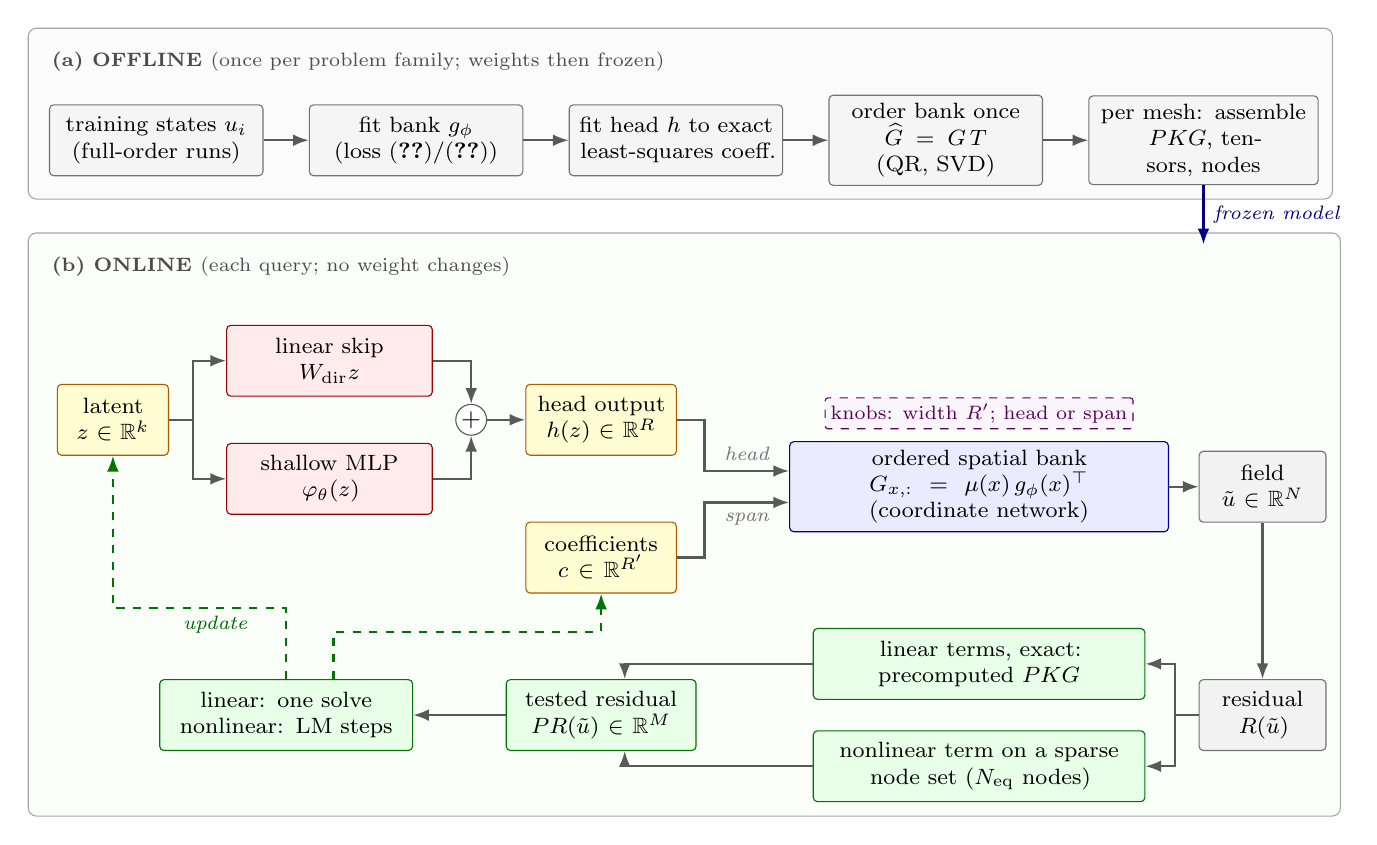
\begin{tikzpicture}[
  font=\footnotesize,
  box/.style={draw, rounded corners=1.5pt, minimum height=9mm, align=center,
              inner sep=3pt},
  off/.style={box, fill=gray!8, draw=black!55, text width=25mm},
  dec/.style={box, fill=red!8, draw=red!60!black, text width=24mm},
  latent/.style={box, fill=yellow!18, draw=orange!70!black},
  bank/.style={box, fill=blue!8, draw=blue!55!black, text width=46mm},
  io/.style={box, fill=gray!10, draw=black!55},
  solve/.style={box, fill=green!9, draw=green!45!black},
  sum/.style={circle, draw=black!65, fill=white, inner sep=0.6pt, font=\small},
  knob/.style={draw=violet!70!black, dashed, rounded corners=1pt, fill=violet!4,
               font=\scriptsize, inner sep=2pt, text=violet!70!black},
  arr/.style={-{Latex[length=2mm]}, thick, draw=black!65},
  upd/.style={-{Latex[length=2mm]}, thick, dashed, draw=green!45!black},
  lbl/.style={font=\scriptsize\itshape, text=black!55},
  row/.style={font=\scriptsize\bfseries, text=black!70, anchor=west},
  panel/.style={draw=black!35, rounded corners=3pt, inner sep=5pt}
]
  % ===== (a) OFFLINE =====
  \node[row] (ta) at (-0.9,4.55) {(a) OFFLINE \textmd{(once per problem family; weights then frozen)}};
  \node[off] (o1) at (0.55,3.55) {training states $u_i$\\(full-order runs)};
  \node[off] (o2) at (3.85,3.55) {fit bank $g_\phi$\\(loss \eqref{eq:bank-loss-joint}/\eqref{eq:bank-loss-vp})};
  \node[off] (o3) at (7.15,3.55) {fit head $h$ to exact\\least-squares coeff.};
  \node[off] (o4) at (10.45,3.55) {order bank once\\$\widehat G=G\,T$ (QR, SVD)};
  \node[off, text width=27mm] (o5) at (13.85,3.55) {per mesh: assemble\\$PKG$, tensors, nodes};
  \draw[arr] (o1) -- (o2); \draw[arr] (o2) -- (o3); \draw[arr] (o3) -- (o4); \draw[arr] (o4) -- (o5);
  \begin{scope}[on background layer]
    \node[panel, fill=gray!3, fit=(ta)(o1)(o5)] {};
  \end{scope}

  % ===== (b) ONLINE =====
  \node[row] (tb) at (-0.9,1.95) {(b) ONLINE \textmd{(each query; no weight changes)}};
  \node[latent, text width=12mm] (z) at (0,0) {latent\\$z\in\Real^{k}$};
  \node[dec] (skip) at (2.75,0.75) {linear skip\\$W_{\mathrm{dir}} z$};
  \node[dec] (mlp) at (2.75,-0.75) {shallow MLP\\$\varphi_\theta(z)$};
  \node[sum] (s1) at (4.55,0) {$+$};
  \node[latent, text width=17mm] (h) at (6.2,0) {head output\\$\head(z)\in\Real^{R}$};
  \node[latent, text width=17mm] (c) at (6.2,-1.75) {coefficients\\$c\in\Real^{R'}$};
  \node[bank] (G) at (11.0,-0.85) {ordered spatial bank\\$\bank_{x,:}=\bcmask(x)\,g_\phi(x)\T$\\(coordinate network)};
  \node[io, text width=14mm] (u) at (14.6,-0.85) {field\\$\tilde u\in\Real^{N}$};

  \draw[arr] (z.east) -- ++(0.3,0) |- (skip.west);
  \draw[arr] (z.east) -- ++(0.3,0) |- (mlp.west);
  \draw[arr] (skip.east) -| (s1.north);
  \draw[arr] (mlp.east) -| (s1.south);
  \draw[arr] (s1) -- (h);
  \draw[arr] (h.east) -- ++(0.35,0) |- ([yshift=2mm]G.west)
       node[pos=0.75, above, lbl] {head};
  \draw[arr] (c.east) -- ++(0.35,0) |- ([yshift=-2mm]G.west)
       node[pos=0.75, below, lbl] {span};
  \draw[arr] (G) -- (u);
  \node[knob, above=1.5mm of G] {knobs: width $R'$; head or span};

  \node[io, text width=14mm] (res) at (14.6,-3.75) {residual\\$R(\tilde u)$};
  \node[solve, text width=40mm] (lin) at (11.0,-3.1) {linear terms, exact:\\precomputed $PKG$};
  \node[solve, text width=40mm] (eq) at (11.0,-4.4) {nonlinear term on a sparse\\node set ($N_{\mathrm{eq}}$ nodes)};
  \node[solve, text width=22mm] (rw) at (6.2,-3.75) {tested residual\\$P R(\tilde u)\in\Real^{M}$};
  \node[solve, text width=30mm] (lm) at (2.2,-3.75) {linear: one solve\\nonlinear: LM steps};

  \draw[arr] (u) -- (res);
  \draw[arr] (res.west) -- ++(-0.3,0) |- (lin.east);
  \draw[arr] (res.west) -- ++(-0.3,0) |- (eq.east);
  \draw[arr] (lin.west) -| ([xshift=3mm]rw.north);
  \draw[arr] (eq.west) -| ([xshift=3mm]rw.south);
  \draw[arr] (rw) -- (lm);
  \draw[upd] (lm.north) -- ++(0,0.9) -| (z.south);
  \draw[upd] ([xshift=6mm]lm.north) -- ++(0,0.6) -| (c.south);
  \node[lbl, text=green!40!black] at (1.3,-2.6) {update};
  \begin{scope}[on background layer]
    \node[panel, fill=green!2, fit=(tb)(z)(u)(eq)(lm)] {};
  \end{scope}
  \draw[arr, draw=blue!50!black] (o5.south) -- ++(0,-0.75) node[right, lbl, text=blue!50!black, pos=0.5] {frozen model};
\end{tikzpicture} {}}
\caption{\rev{NM-ROM, redrawn with the two stages separated.
\textbf{(a) Offline, once per problem family:} fit the coordinate-network
bank to full-order training states (Appendix~\ref{app:bank-loss}), fit the
head to their exact least-squares bank coefficients, order the bank once,
and assemble tests, reduced operators and nonlinear-term nodes for each
mesh; all of it is charged as offline cost (Table~\ref{tab:breakeven}).
\textbf{(b) Online, each query:} the head maps a latent code $z$ to bank
coefficients, $\tilde u=G\,h(z)$, or the span of the first $R'$ ordered
columns gives $\tilde u=\widehat G_{R'}c$; the residual, tested against
$M$ fixed tests $P$ with precomputed linear terms and a sparse node set for
the nonlinear term, is solved by one least-squares solve (linear PDE in the
span) or Levenberg--Marquardt steps. Dashed tag: choices made at query
time.}}
\label{fig:decoder}
\end{figure}

\paragraph{Projection-based ROMs.}
Linear ROMs approximate solutions in a fixed subspace
\citep{BennerGugercinWillcox2015,Sirovich1987POD}; moving fronts can
require a large basis \citep{CohenDeVore2015,GreifUrban2019,Peherstorfer2022Kolmogorov}.
Nonlinear-manifold ROMs replace the subspace by a learned manifold and
keep the residual projection
\citep{LeeCarlberg2020,KimChoi2022NMROM,Romor2023NMROM,Diaz2024DDNMROM},
including quadratic manifolds \citep{GeelenWrightWillcox2022,BarnettFarhat2022},
neural-network corrections to a linear basis \citep{Barnett2023NNPROM},
adaptive bases \citep{PeherstorferWillcox2015Adaptive,Carlberg2015hRefinement},
hyper-reduced models of Navier--Stokes flows \citep{Romor2025Explicable}
and graph autoencoders on unstructured meshes \citep{Magargal2025GraphAE}.
These methods solve the PDE online\rev{; a linear or quadratic basis is
stored on the mesh it was built on, though it can be interpolated to
another}, and an autoencoder decoder is evaluated
at every node in each online iteration unless it is hyper-reduced.
Latent-dynamics ROMs instead learn the reduced dynamics from data
\citep{Fries2022LaSDI,He2023gLaSDI}.
Least-squares Petrov--Galerkin projection \citep{Carlberg2011LSPG} and
preassembly of reduced operators
\citep{StefanescuSandu2014,WederSchwerdtnerPeherstorfer2024} are
established components that we reuse. Our closest relatives are
neural-field ROMs \citep{Chen2023CROM,KimWenLeeChoiCNFROM2024,Berman2024CoLoRA}, which
also evaluate a coordinate network at individual nodes\rev{; we compare
with a CROM-style and a CoLoRA-style model in
\S\ref{sec:results:baselines}}. We differ in
three ways: our decoder separates space from the latent code (a bank
times a head), so every linear term is precomputed exactly; the bank
carries an exact Dirichlet factor \rev{(on the cylinder, a product of
smooth distance factors to the boundary pieces, with the inflow carried by
a lift function)}; and the bank is ordered after
training, so its nested widths give accuracy settings at query time
from one trained model, as runtime-tunable networks do for vision and
language models
\citep{YuSlimmable2019,Cai2020OnceForAll,Kusupati2022MRL,Devvrit2024MatFormer}.

\paragraph{Neural operators.}
FNO \citep{Li2020FNO}, DeepONet \citep{Lu2021DeepONet}, U-Net
\citep{Ronneberger2015UNet,Takamoto2022PDEBench} and Transolver
\citep{WuTransolver2024,Luo2025Transolverpp} learn solution maps, as do
neural-field operators \citep{Serrano2023CORAL} and pretrained PDE
foundation models \citep{Herde2024Poseidon,Hao2024DPOT}.
Their resolution or inference procedure can change accuracy and cost;
our accuracy setting instead changes the trial space in which the PDE
residual is solved.

\paragraph{Hyper-reduction and baselines.}
Empirical quadrature \citep{Hernandez2017EQ,YanoPatera2019LPEQ,Hernandez2024CECM}
and energy-conserving sampling and weighting \rev{(ECSW)
\citep{Farhat2014ECSW}} reduce nonlinear residual evaluation through
non-negative weights; we \rev{describe that construction, test every
rule, fitted or not, on the states the solver reaches, and use a fixed
uniform sub-lattice where it suffices (\S\ref{sec:method:precomp})}.
Because learned solvers are often compared with weak baselines
\citep{McGreivy2024Weak}, we compare \rev{each setting with the fastest
configuration of a solver ladder that is at least as accurate, including
coarser meshes and, on box problems, sine-transform solvers}.


\section{Methodology}\label{sec:method}
\edef\restoredisplays{%
  \noexpand\abovedisplayskip=\the\abovedisplayskip
  \noexpand\belowdisplayskip=\the\belowdisplayskip
  \noexpand\abovedisplayshortskip=\the\abovedisplayshortskip
  \noexpand\belowdisplayshortskip=\the\belowdisplayshortskip}
\setlength{\abovedisplayskip}{1pt plus 1pt minus 1pt}
\setlength{\belowdisplayskip}{1pt plus 1pt minus 1pt}
\setlength{\abovedisplayshortskip}{1pt plus 1pt minus 1pt}
\setlength{\belowdisplayshortskip}{1pt plus 1pt minus 1pt}

A full-order solve has one unknown per grid node, so its cost grows with
the mesh size $N$. For each query we instead solve the same discretised
PDE in a few unknowns, at a cost that barely depends on $N$ \rev{apart
from forming the output field}. This needs
three ingredients. First, a compact set of candidate solutions, the trial
manifold (\S\ref{sec:method:manifold}): the solution is a weighted sum of
the functions in the spatial bank, and its weights are either produced by
the nonlinear head from a few latent unknowns or solved for directly on
the first $R'$ bank functions. Second, a way to choose the right
candidate without knowing the answer (\S\ref{sec:method:weak}). Third, a
way to evaluate the PDE without visiting all $N$ nodes
(\S\ref{sec:method:precomp}): linear terms are computed once offline, and
the nonlinear term is sampled at a few nodes (in three dimensions, it is
evaluated with a precomputed quadratic tensor). Figure~\ref{fig:decoder} shows the whole pipeline. Throughout, $u\in\Real^{N}$ is the full-order discrete state
on a uniform grid and $K\in\Real^{N\times N}$ is the sparse
finite-difference matrix of $-\Delta$.



\subsection{Trial Manifold with Exact Dirichlet Enforcement}
\label{sec:method:manifold}

Solutions of one PDE family share their spatial structure, so a few
learned functions of space can describe all of them; the nonlinear head
lets their combination follow features, such as moving fronts, that a
small fixed combination misses. We do not use an encoder. The decoder writes the state as a fixed set of
spatial functions times coefficients produced by a small network,
\begin{equation}
  \tilde u(z) = \mathcal D(z) = G\,h(z),
  \qquad
  G_{x,:} = \mu(x)\,g_\phi(x)\T,
  \qquad
  \mu(x) = 16\,x_1(1-x_1)\,x_2(1-x_2).
  \label{eq:bank}
\end{equation}
Each column of the bank $G\in\Real^{N\times R}$ is one spatial function.
The function comes from a small network $g_\phi$ that takes the
coordinates of a point and returns a value there, so a column is simply
that network evaluated at every grid node. The head
$h:\Real^{k}\to\Real^{R}$ takes the latent state $z$ and returns one
weight per column. Because $\mu$ is zero on the boundary $\Gamma$, every
column of $G$ is zero there too. The boundary values therefore never
change when $z$ changes, on any mesh, and the boundary equations do not enter the solve. 
%The cube and the L-shaped domain use their own factor, which is zero on their boundaries in the same way. 
The cube and the L-shaped domain define their own boundary factor (Appendix~ \ref{app:method}), zero on their boundaries in the same way. \rev{On the cylinder the factor is a product of smooth distance factors to the inlet, the channel walls and the cylinder surface, which can be formed for any boundary whose distance can be computed; the inflow is carried by a lift function and the bank represents the remainder (Appendix~\ref{app:method:cyl}).}
%For each new problem, we find $z$ by solving the PDE 
Each query then solves for $z$ (head) or $c$ (span) by solving the PDE
(\S\ref{sec:method:weak}).

\paragraph{Ordering the bank.}
\label{sec:method:ladder}\label{sec:method:ordered}
Training does not rank the columns of $G$, so after training we replace
them by combinations sorted from most to least important,
\begin{equation}
  \widehat G = G\,T .
  \label{eq:ordered}
\end{equation}
The matrix $T$ comes from a principal component analysis of the training
fields written in the bank (Appendix~\ref{app:method:ordered}). Keeping
the first $R'$ columns gives the best $R'$-dimensional subspace of the bank for the training data. At full width nothing changes: $\widehat G$
spans the same space as $G$, and no weight is retrained.
A query then solves in one of two ways,
\begin{equation}
  \tilde u = G\,h(z),\;\; z\in\Real^{k}
  \quad(\text{head}),
  \qquad
  \tilde u = \widehat G_{R'}\,c,\;\; c\in\Real^{R'}
  \quad(\text{span}),
  \label{eq:modes}
\end{equation}
where $\widehat G_{R'}$ holds the first $R'\le R$ columns. The head is a
nonlinear manifold with $k$ unknowns; the span is a linear space with $R'$
unknowns. The width $R'$ is the accuracy knob. The columns are nested, so
narrowing the span needs no retraining, and cheaper to solve and to convert back to a field.

\subsection{Projecting the PDE onto the Manifold}
\label{sec:method:weak}

At query time the solution is unknown but the PDE is known, so we choose
the candidate that best satisfies the discretised equations; no solution
data is needed at query time. Each PDE we consider gives a discretised residual $R(u)$ that vanishes at
the discrete solution. We substitute the trial manifold into $R$ and,
%instead of projecting with the decoder Jacobian, 
instead of pulling the residual back through the decoder Jacobian,
test it against $M$ fixed
vectors, the rows of $P\in\Real^{M\times N}$. On the square these are the
$M$ lowest sine modes, which are eigenvectors of $K$. 
%
% A query solves
A head query solves
\begin{equation}
  z^{\star} = \argmin_{z}\;\tfrac12\,\norm{P\,R\big(\tilde u(z)\big)}_2^2;
  \label{eq:objective}
\end{equation}
a span query solves the same problem in $c$.
We choose $M$ with the width: $M\ge k$ for the head and $M\ge R'$ for the span ($M=4R'$ for Burgers). 
%
This is least-squares Petrov--Galerkin projection \citep{Carlberg2011LSPG,LeeCarlberg2020} with fixed rather than state-dependent tests; each
row of $PR$ is also scaled by a fixed factor that puts the tests on a
common scale (Appendix~\ref{app:method}); we leave this scaling out of the
notation. We solve \eqref{eq:objective} by
damped Gauss--Newton (Levenberg--Marquardt) \citep{Marquardt1963},
\begin{equation}
  \Delta z = -\big(J\T J+\lambda\,\diag(J\T J)\big)^{-1}J\T P\,R\big(\tilde u(z)\big),
  \qquad
  J = P\,\frac{\partial R}{\partial u}\,J_{\mathcal D}(z),
  \label{eq:lm}
\end{equation}
and keep a step only if the residual decreases. Here
$J_{\mathcal D}(z)=G\,J_h(z)$ for the head and $J_{\mathcal D}=\widehat
G_{R'}$, a constant, for the span. Unlike $J_{\mathcal D}(z)\T$, the tests
$P$ do not change with $z$, which is what lets every linear term be
computed once (\S\ref{sec:method:precomp}). For Poisson in the span,
\eqref{eq:objective} is a linear least-squares problem solved once, and for
heat in the span each step is linear; the iteration is needed only for the
head and for the nonlinear PDEs.

\paragraph{Elliptic (Poisson).}
In the span the Poisson residual $R(u)=Ku-F$ is linear in $c$, so a query
is one least-squares solve with the fixed matrix $PK\widehat G_{R'}$
(Appendix~\ref{app:method:poisson}).

\paragraph{Time-dependent problems.}
Heat (Crank--Nicolson), Burgers (backward Euler with a sign-upwind
stencil) and Navier--Stokes (implicit midpoint on the periodic cube) each
give a residual $R(u_{n+1})$ for one time step; their forms are in
Appendix~\ref{app:method}. Each step solves
\begin{equation}
  z_{n+1} = \argmin_{z}\;\norm{P\,R\big(\tilde u(z)\big)}_2,
  \qquad u_n=\tilde u(z_n),
  \label{eq:step}
\end{equation}
by \eqref{eq:lm}, warm-started from the previous step; the span solves the
same problem in $c_{n+1}$. The heat residual is linear, so in the span the
rollout applies one fixed $R'\times R'$ matrix per step. Burgers and
Navier--Stokes add a nonlinear advection term $A(u)$, so both the head and
the span iterate \eqref{eq:lm} at every step. For Navier--Stokes the tests
$P$ are divergence-free Fourier modes, so the pressure drops out of $PR$;
because the vortices travel, the bank is evaluated in a frame centred on
the flow whose shift is solved at each step (Appendix~\ref{app:method:ns}).

\subsection{Hyper-reduction}
\label{sec:method:precomp}

The manifold reduces the unknowns from $N$ to $k$ or $R'$, but the tested
residual $P\,R(\tilde u)$ still visits every node, so each evaluation costs
$O(NR)$, which would erase the wall-clock benefit. We remove this cost in two
ways, one for linear terms and one for the nonlinear term.

\paragraph{Linear terms: computed once and exact.}
A linear term is tested once, offline. For the Laplacian,
\begin{equation}
  P K\tilde u = \big(PKG\big)\,h(z),
  \qquad PKG\in\Real^{M\times R},
  \label{eq:preassembled}
\end{equation}
and the span uses $PK\widehat G_{R'}$, the first $R'$ columns of
$PKG\,T$. Online a linear term costs $O(MR)$ and is exact. For Poisson and
heat this is the whole residual, so their reduced solves make no
approximation beyond the trial space.

\paragraph{The nonlinear term: Empirical Quadrature.}
The advection terms of Burgers and Navier--Stokes cannot be computed once. We use Empirical Quadrature
\citep{Hernandez2017EQ,YanoPatera2019LPEQ} to select a non-negative
per-node weight vector $w$, independent of the state, such that
\begin{equation}
  P A(\tilde u) = \sum_{i=1}^{N} P_{:,i}\,A_i(\tilde u)
  \;\approx\; \sum_{i\in\mathcal S} w_i\,P_{:,i}\,A_i(\tilde u).
  \label{eq:eq-rule}
\end{equation}
It is fitted by non-negative least squares on states the solver reaches on training trajectories (Appendix~\ref{app:method:eq}), giving a support $\mathcal S$ of $N_{\mathrm{eq}}\ll N$ nodes. \rev{Where a
simpler rule passes the same check we use it instead: the Burgers 2D rows
of Table~\ref{tab:headline} use a fixed uniform $63{\times}63$ interior
lattice with equal weights and no fit, which reduces the query at
$1024^2$ from 1,263 to 49.3\,ms at unchanged error.} The decoder is evaluated only on $\mathcal S$ and its stencil
neighbours, $\mathcal S^{+}$; those rows of the bank are computed once and
cached.

\paragraph{Cost.}
With linear terms computed once and advection on $\mathcal S^{+}$, one
iteration of \eqref{eq:lm} costs
\begin{equation}
  \mathcal O\big(MR\,(N_{\mathrm{eq}}+k)\big),
  \label{eq:cost}
\end{equation}
with $k$ replaced by $R'$ in the span, plus the cost of the head and of
the small normal-equation solve, none of which depends on $N$. Returning the
field at an output time is one further $O(NR')$ product.

\paragraph{Checking the rule.}
Each rule is checked on the states the reduced solver reaches on
held-out trajectories, against an error bar fixed in advance\rev{; the
lattice of the Burgers rows and the quadratic tensors of the 3D rows pass
it (Appendix~\ref{app:method:eq})}.

\subsection{Model Architecture}
\label{sec:decoder}

Two requirements shape the model in Figure~\ref{fig:decoder}: the head
solve needs a usable Jacobian at its stored starting code, and a sparse
node set saves time only if the decoder can be evaluated at one node
without the others\rev{; the learned functions are then also shared by the
meshes of a series, while the reduced operators are assembled once per
mesh}.
Widths and training
settings are in Appendix~\ref{app:training-schedule}.

\paragraph{Linear skip, for the latent solve.}
The head is a shallow network plus a linear map,
\begin{equation}
  \head(\latent) \;=\; W_{\mathrm{dir}}\latent \;+\; \varphi_\theta(\latent),
  \qquad
  \varphi_\theta(\latent)=W_3\,\sigma\big(W_2\,\sigma(W_1\latent+b_1)+b_2\big)+b_3,
  \label{eq:head}
\end{equation}
with $\sigma$ the SiLU activation. Its Jacobian is
$\dhead(\latent)=W_{\mathrm{dir}}+J_{\varphi}(\latent)$. The first term does not
depend on $\latent$, so \rev{the first Levenberg--Marquardt step from a
stored code has a non-zero linear direction even where $J_\varphi$ is
small (this does not guarantee convergence)}, while $\varphi_\theta$
supplies the curvature of the manifold. The head acts on the $R$ bank
coefficients, not on the $N$ nodes, so its cost and its parameter count do
not depend on the mesh.

\paragraph{Coordinate-network bank, for node-local evaluation.}
Each column of the bank is a coordinate network read at the node and
multiplied by the boundary factor of \eqref{eq:bank},
\begin{equation}
  \bank_{x,r}=\bcmask(x)\,g_{\phi,r}(x),
  \qquad
  g_\phi(x)=\mathrm{MLP}_\phi\big(\gamma(x)\big),
  \quad
  \gamma(x)=\big[\cos(2\pi\Omega x),\;\sin(2\pi\Omega x)\big],
  \label{eq:coordnet}
\end{equation}
where $\gamma$ is a random-Fourier-feature embedding
\citep{Tancik2020FourierFeatures} \rev{whose frequency matrix $\Omega$
is initialised at random and then trained for Burgers 2D, Poisson 2D and
the L-shape, and kept fixed for the other problems (Appendix~\ref{app:bank-loss})}. Because
$g_\phi$ reads a coordinate, a row of $\bank$ is computed from its node
alone. A quadrature rule therefore needs only the rows of $\mathcal S^{+}$,
and the same trained network is sampled on every mesh.

\label{sec:method:tuning}\label{sec:method:layers}
\subsection{Implementation and Training}
\label{sec:impl}
Online, $J=PKG\,J_h(z)$ with the head Jacobian from forward-mode
automatic differentiation in JAX \citep{Bradbury2018JAX}, and each accepted
step solves the small damped normal equation directly. Training uses training data only: the
coordinate network $g_\phi$ is fitted \rev{by minimising the relative
reconstruction error of the training states in its span, with a small
conditioning penalty on its columns (\eqref{eq:bank-loss-joint} and
\eqref{eq:bank-loss-vp} in Appendix~\ref{app:bank-loss})}, and frozen; the
head is then fitted to the \rev{exact least-squares} bank
coefficients of those states, with one stored code per training state (an
auto-decoder); last, the bank is ordered once by \eqref{eq:ordered}, with
one QR and one SVD. \rev{At query time the coefficients come from the
projected PDE solve, never from the reference.} Widths, cohorts and offline costs are in
Appendix~\ref{app:training-schedule}.

% =====================================================================
\section{Experimental Setup and Benchmark Problems}
\label{sec:setup}
\restoredisplays

\paragraph{Problems and references.}
\begin{revblock}
The speed case rests on two problems that a coarse mesh does not resolve.
(i) \emph{Navier--Stokes 3D, harder family}: incompressible flow on the
periodic cube with a quarter of the viscosity of our original family
($\nu\sim\log U(5{\times}10^{-4},2.5{\times}10^{-3})$) and four times
sharper vortex blobs, horizon $T=0.2$, reference CNAB2 at $192^3$
(Appendix~\ref{app:method:nshard}), chosen from five candidate families by
criteria fixed before any reduced model was run; evaluated at $64^3$, $96^3$ and
$128^3$. (ii) \emph{Unsteady flow past a cylinder} (DFG 2D-2 geometry
\citep{SchaeferTurek1996}): vortex shedding on P2/P1 finite elements with
96,781 unknowns, trained at Reynolds numbers 90, 100 and 110, settings
frozen at 95, held-out 105 (Appendix~\ref{app:method:cyl}). We also report
the submission's problems: Burgers 2D/3D, the original Navier--Stokes
family, Poisson on an L-shape, and, as correctness checks, Poisson and
heat on boxes (Appendix~\ref{app:boxes}).
\end{revblock}
Meshes and cohorts are in
Table~\ref{tab:problems}, the sampled families in Table~\ref{tab:spec} and
the three-dimensional configurations in Table~\ref{tab:config3d}.

\paragraph{Accuracy.}
We report the worst relative $L^2$ error over the stated cases and
requested times, in percent. Poisson uses the steady reference norm and
heat the current reference norm; Burgers and Navier--Stokes use the
initial-field norm over evolved times\rev{; the cylinder uses six fixed
acceptance targets (velocity RMS and maximum error, pressure error,
Strouhal number, maximum drag and maximum lift)}. \rev{Test cohorts have
16 to 128 cases. In every new experiment (\S\ref{sec:results:ns}--\ref{sec:results:baselines})
the settings were frozen on development cases before the held-out cases
were evaluated; tables on six development cases are labelled as such.}

\paragraph{Timing, speedup and matched solvers.}
Each accuracy--time pair comes from one invocation, with warm-up,
synchronisation and medians of repetitions (Appendix~\ref{app:cg-current}). Training, data generation and
per-mesh assembly are offline costs (Table~\ref{tab:breakeven}).
\rev{Speedup divides the time of a \emph{matched} solver by the model's:
the fastest configuration of a solver ladder whose worst error on the same
cases is at or below the setting's own. On the harder Navier--Stokes family
the ladder has 450 configurations of a GPU Fourier pseudo-spectral solver
over mesh ($32^3$--$128^3$), integrator (CNAB2, RK4) and step; on the cylinder, 62 finite-element configurations
over mesh, element order, integrator, step and refresh interval; on the
original benchmarks, the named solver's own ladder (CG, Crank--Nicolson CG,
Newton--BiCGStab, CNAB2), with sine-transform solvers reported where
measured. Spread is in Appendix~\ref{app:spread}.}

\section{Numerical Experiments and Results}\label{sec:results}
\rev{We ask where the model is faster than a solver of the same accuracy
(\S\ref{sec:results:ns}--\ref{sec:results:fom}), how it compares with
neural-field ROMs and neural operators (\S\ref{sec:results:baselines}),
and what each component contributes (\S\ref{sec:results:tunability}).}

% ---------------------------------------------------------------------
\subsection{Interacting Vortices in Three-Dimensional Navier--Stokes}\label{sec:results:ns}

\begin{table}[t]
\centering
\color{blue}
\caption{\textbf{Harder Navier--Stokes family}, 128 fresh test cases,
three independently trained models (trajectories, per-mesh POD banks and
heads re-drawn), settings frozen on 64 development cases. Errors: range
over three seeds. Times: seed~0, median over eight cases, online solve
only (spread in Table~\ref{tab:spread-g1}). Speedup over the fastest
configuration of a 450-entry solver ladder (any mesh to $128^3$, CNAB2 or
RK4, any step) at least as accurate on the same cases; range over the two
seeds that passed the timing-stability check. \emph{Fast}: fewer steps
or tests, also frozen on development cases.}
\label{tab:g1}
\scriptsize\setlength{\tabcolsep}{3.5pt}
\begin{tabular}{@{}lllll@{}}
\toprule
Head on a per-mesh & Worst-case error, three seeds & Median & Time & Speedup over matched solver \\
POD bank of width & $64^3$ / $96^3$ / $128^3$ (\%) & error (\%) & $64^3$ / $96^3$ / $128^3$ (ms) & $64^3$ / $96^3$ / $128^3$ \\
\midrule
64 & 1.17--1.36 / 1.45--1.61 / 1.43--1.69 & 0.34--0.54 & 16 / 17 / 31 & 6.9 / 6.4--6.5 / 3.6--3.7$\times$ \\
96 & 0.58--0.75 / 0.64--0.78 / 0.62--0.82 & 0.17--0.19 & 17 / 26 / 43 & 9.4--11.7 / 7.6--9.5 / 4.7--6.9$\times$ \\
128 & 0.42--0.60 / 0.43--0.62 / 0.45--0.64 & 0.10--0.12 & 31 / 48 / 62 & 6.3--6.5 / 5.2--7.0 / 4.0--5.3$\times$ \\
128, fast & 0.49--0.67 / 0.52--0.68 / 0.47--0.69 & 0.12--0.14 & 19 / 31 / 51 & 9.4--10.4 / 8.0--10.9 / 4.9--6.1$\times$ \\
192 & 0.28--0.39 / 0.35--0.41 / 0.35--0.42 & 0.06--0.08 & 52 / 67 / 121 & 3.9--5.9 / 5.9--6.2 / 3.3--3.4$\times$ \\
192, fast & 0.35--0.48 / 0.39--0.47 / 0.43--0.47 & 0.09--0.11 & 25 / 40 / 68 & 8.0--10.2 / 8.3--10.0 / 5.1$\times$ \\
\midrule
Linear span, same banks & 7.7--70 & --- & --- & 0.04--0.56$\times$ \\
\bottomrule
\end{tabular}
\end{table}

\begin{revblock}
The periodic unit cube contains two interacting vortex blobs, with sharpness
$\beta=8$ and viscosity $\nu\in[5\times10^{-4},2.5\times10^{-3}]$.
Relative to the original family, the blobs are narrower and the viscosity
is four times lower. The family was selected by resolution and representation
criteria fixed before reduced-model runs (Appendix~\ref{app:method:nshard}).
Figure~\ref{fig:ns-head-span} compares the head and the same bank's span.

In Table~\ref{tab:g1} the fast width-192 setting is below 0.5\,\% on every
mesh and seed and 5.1--10.2$\times$ faster than the matched solver, which
needs meshes of $100^3$ to $120^3$.
Across all settings the head is 3.3--11.7$\times$ faster than its matched
solver. The nonlinear head is what makes this work: the linear span of the
same bank is unstable, more so as the bank widens, and slower than the
solver. Median errors differ by less than 0.03 percentage points between
seeds at widths 96 and above. The speedup narrows with mesh and width
(3.3$\times$ for width 192 at $128^3$). The third seed's timing run failed
a timing-stability check twice; its ratios (3.4--10.6$\times$) lie in the
same range.

\paragraph{One coordinate network for all meshes.} Table~\ref{tab:g1} uses
per-mesh POD banks. On an earlier 32-case cohort one coordinate network
fitted once replaces them on all three meshes at 0.90/1.23/1.39\,\% and
14.2/6.7/3.8$\times$, level with per-mesh POD except at $128^3$
(1.17\,\%, 6.1$\times$); with its $64^3$ head reused it gives
1.05/1.06\,\% at $96^3$/$128^3$ (Table~\ref{tab:coordnet}).
\end{revblock}

% ---------------------------------------------------------------------
\begin{figure}[t]
\centering
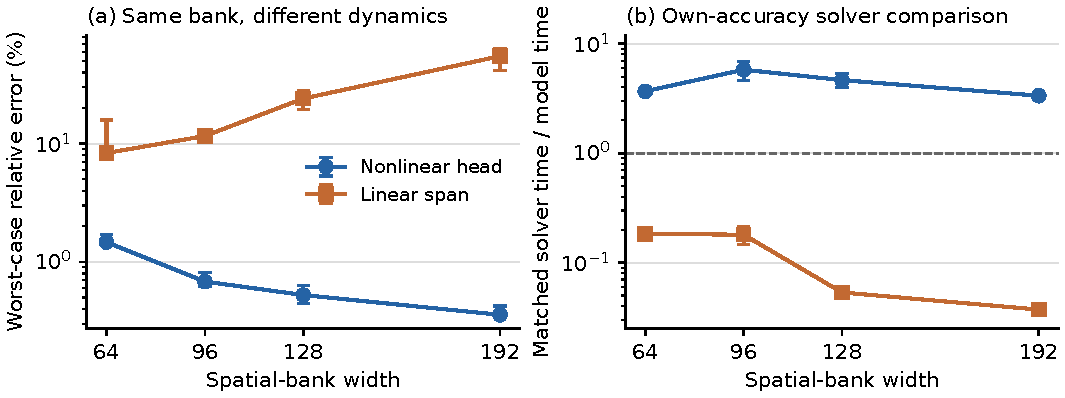
\includegraphics[width=\linewidth]{figs/F8_ns_head_span.pdf}
\caption{\rev{The nonlinear head changes the dynamics within the same bank.
Navier--Stokes at $128^3$, using the fresh cohort of Table~\ref{tab:g1}.
Left: worst-case cohort error, median and range across three independently
trained models. Right: speedup over each setting's own accuracy-matched
pseudo-spectral solver, median and range over the two models passing the
timing gate at every mesh; dashed line: equal cost.
These are the accurate head settings, not the fast rows.}}
\label{fig:ns-head-span}
\end{figure}

\subsection{Unsteady Flow past a Cylinder}\label{sec:results:cyl}

\begin{table}[t]
\centering
\color{blue}
\caption{\textbf{Cylinder flow, held-out Reynolds number 105.} One trained
bank at three widths, rollout over 1.7\,s (five shedding periods).
Comparator: cheapest finite-element run meeting all six targets, screened
from a 62-entry ladder on the development case and re-checked at Re 105
(coarser P3/P2 mesh, 16,912 unknowns). Every row meets all six targets.
Medians of five repetitions on one 16-thread CPU node (ranges: 37.5--49.4,
1.69--1.72, 0.82--0.83, 0.79\,s). \emph{With field output}: velocity
rebuilt at all 681 saves.}
\label{tab:g2}
\small\setlength{\tabcolsep}{4pt}
\begin{tabular}{@{}lccc@{}}
\toprule
Setting & Velocity error & Rollout time & Speedup (rollout / with field output) \\
\midrule
Cheapest passing finite-element run & $9.4{\times}10^{-3}$ & 42.2\,s & 1$\times$ \\
Width 32, step 1/400 & $7.0{\times}10^{-3}$ & 1.71\,s & 24.7$\times$ / 11.2$\times$ \\
Width 24, step 1/400 & $5.5{\times}10^{-3}$ & 0.83\,s & 51.2$\times$ / 15.9$\times$ \\
Width 16, step 1/800 & $8.3{\times}10^{-3}$ & 0.79\,s & 53.6$\times$ / 17.6$\times$ \\
\bottomrule
\end{tabular}
\end{table}

\begin{revblock}
Training and evaluation use a P4/P3 Taylor--Hood reference at step 1/3200;
the reduced model is built on a P2/P1 export mesh with 96,781 unknowns.
The accuracy-matched finite-element comparator is a separate, cheaper
configuration (Table~\ref{tab:g2}).
On a non-box geometry one trained bank meets all six targets at every
width (Table~\ref{tab:g2}), with a rollout 25--54$\times$ faster than the
cheapest finite-element run that meets the same targets (11--18$\times$
including field output); with a finer step width 32 reaches
$1.9{\times}10^{-3}$. Over a window three times longer, widths 24 and 32
still meet all six targets ($4.0{\times}10^{-3}$ and $2.4{\times}10^{-3}$
at step 1/800), while the best of six neural operators trained for this
comparison meets three. At Reynolds 80 and 120, outside the band,
width 32 meets five and four targets ($1.2{\times}10^{-2}$ against
$10^{-2}$), narrower widths one to three and the best operator three and
four (Table~\ref{tab:cyl-extra}). The bank's boundary factor is a product of
distance factors, the inflow is in a lift function, the rollout is
Galerkin (Appendix~\ref{app:method:cyl}), and a POD basis of equal width
performs the same.
Replacing the comparator's sparse LU with the tested CPU algebraic-multigrid
variants preserves all targets but is slower, so LU remains the stronger
measured baseline (Appendix~\ref{app:method:cyl}).
\end{revblock}

% ---------------------------------------------------------------------
\subsection{Original Benchmarks against Matched Solvers}\label{sec:results:fom}
\label{sec:results:operators}\label{sec:exp:panel}

\begin{table}[t]
\centering
\color{blue}
\caption{The submission's benchmarks, each setting against the solver
matched to \emph{its own} error within that problem's original solver
ladder. \textbf{Both NM-ROM columns of a row come from one frozen model}:
\emph{accurate} is the most accurate tested setting, fixed before the
test cases were opened. \emph{Fast$^\dagger$} is the cheapest tested
width whose worst error on these test cases is below 5\,\% (L-shape
5.6\,\%): \textbf{it was selected using the test errors}, so its error is
not a held-out estimate. Error is the worst relative $L^2$ error over the
test cases (\%). Speedup: matched solver's median time over the NM-ROM's,
same GPU allocation, \textbf{bold} where the NM-ROM is faster; timing
spread in Table~\ref{tab:spread-t1}. Box Poisson and heat are in
Table~\ref{tab:boxes}. Burgers 2D uses a fixed $63{\times}63$ lattice for
the nonlinear term (\S\ref{sec:method:precomp}).}
\label{tab:headline}
\scriptsize\setlength{\tabcolsep}{3pt}
\begin{tabular}{@{}llrrrrr@{\hspace{10pt}}llrrrrr@{}}
\toprule
 & & \multicolumn{2}{c}{Accurate} & \multicolumn{2}{c}{Fast$^\dagger$} & FOM & & & \multicolumn{2}{c}{Accurate} & \multicolumn{2}{c}{Fast$^\dagger$} & FOM \\
\cmidrule(lr){3-4}\cmidrule(lr){5-6}\cmidrule(lr){10-11}\cmidrule(lr){12-13}
Problem & Mesh & Err. & Speedup & Err. & Speedup & Err. & Problem & Mesh & Err. & Speedup & Err. & Speedup & Err. \\
\midrule
L-shape & $256^2$ & 2.02 & \textbf{32.1$\times$} & 5.61 & \textbf{29.9$\times$} & 1.08 & Burgers 3D & $64^3$ & 1.01 & 0.21$\times$ & 3.37 & 0.93$\times$ & 0.92 \\
 & $512^2$ & 2.00 & \textbf{50.1$\times$} & 5.60 & \textbf{48.7$\times$} & 0.74 & & $128^3$ & 1.46 & 0.57$\times$ & 4.26 & \textbf{2.87$\times$} & 1.39 \\
 & $1024^2$ & 1.99 & \textbf{41.6$\times$} & 5.60 & \textbf{49.4$\times$} & 1.77 & & $256^3$ & 2.20 & \textbf{2.19$\times$} & 3.77 & \textbf{5.60$\times$} & 1.52 \\
\cmidrule(l){8-14}
 & $2048^2$ & 1.99 & \textbf{78.4$\times$} & 5.60 & \textbf{97.5$\times$} & 1.18 & Navier--Stokes & $32^3$ & 0.21 & 0.93$\times$ & 3.06 & \textbf{3.56$\times$} & 0.19 \\
\cmidrule(r{10pt}){1-7}
Burgers 2D & $256^2$ & 0.87 & 0.38$\times$ & 3.85 & 0.58$\times$ & 0.11 & (original & $64^3$ & 0.21 & \textbf{2.92$\times$} & 3.06 & \textbf{8.53$\times$} & 0.12 \\
 & $512^2$ & 1.13 & 0.62$\times$ & 4.10 & 0.88$\times$ & 0.12 & family) & $96^3$ & 0.21 & \textbf{8.01$\times$} & 3.24 & \textbf{14.4$\times$} & 0.056 \\
 & $1024^2$ & 1.25 & \textbf{1.51$\times$} & 4.25 & \textbf{1.70$\times$} & 0.13 & & & & & & & \\
 & $2048^2$ & 1.32 & \textbf{3.39$\times$} & 3.06 & \textbf{4.43$\times$} & 0.13 & & & & & & & \\
 & $4096^2$ & 1.35 & \textbf{10.7$\times$} & 3.11 & \textbf{13.9$\times$} & 0.14 & & & & & & & \\
\bottomrule
\end{tabular}
\end{table}

\begin{revblock}
Against its own matched solver on the same mesh the fast setting is
faster in 27 of the 30 cells of the submission's Table~1 (which include
the box rows of Table~\ref{tab:boxes}); it is slower on Burgers 2D at
$256^2$ and $512^2$ (0.58, 0.88$\times$) and Burgers 3D at $64^3$
(0.93$\times$), and at Burgers 2D $4096^2$ it falls from 27.5 to
13.9$\times$ (Figure~\ref{fig:matched}). On the original Navier--Stokes
family a solver free to coarsen its mesh (RK4 on $32^3$--$48^3$) gives the
head 0.63/1.65/0.94$\times$ at $32^3$/$64^3$/$96^3$, which is why we moved
to the harder family: the advantage appears where a coarse mesh no longer
suffices. Transform solvers are faster than our model on box Poisson 2D
(0.14--5.05\,ms, 1.8--10$\times$ faster) and 3D and on heat 3D (fast
setting at 0.50--0.61$\times$); our fast setting is 1.1--1.4$\times$
ahead on heat 2D; on Burgers 2D a pseudo-spectral solver is faster up to
$1024^2$ and slower from $2048^2$ (development cases). Box Poisson and heat
are therefore correctness checks (Appendix~\ref{app:boxes}).
\end{revblock}

% ---------------------------------------------------------------------
\subsection{Neural-Field ROMs and Neural Operators}\label{sec:results:baselines}
\label{sec:results:neuralops}

\begin{table}[t]
\centering
\color{blue}
\caption{Burgers 2D at $256^2$, 64 held-out test cases, settings of every
method frozen on validation data. The CROM- and CoLoRA-style models are
our re-implementations. The CoLoRA-style model is given the five
parameters that generate the initial condition and solves no equation
online; ours takes an initial field. FNO and U-Net are trained on exactly
the 4,608 trajectories our head uses, for up to 8.1 hours each (a
4.6-hour run plus one 3.5-hour continuation); most of these runs reached their
time budget before our convergence rule, so these measure budget-limited
performance, not convergence. The 128-trajectory rows rerun the submission's data budget.}
\label{tab:baselines}
\scriptsize\setlength{\tabcolsep}{4pt}
\begin{tabular}{@{}llrrr@{}}
\toprule
Method & Training trajectories & Worst (\%) & Median (\%) & ms / query \\
\midrule
Ours, linear span, width 384 & 576 (bank) + 4,608 & 0.875 & 0.026 & 45.2 \\
Ours, nonlinear head, 16 coordinates & 4,608 & 4.10 & 0.67 & 32.4 \\
CROM-style, 16 coordinates, accurate / fast setting & same & 22.4 / 16.9 & 0.43 / 1.11 & 2,818 / 507 \\
CoLoRA-style regression, 16 & same & 0.240 & 0.104 & 49.9 \\
FNO, variant selected on validation (one seed) & 4,608 & 0.48 & 0.19 & 6.6 \\
FNO, paper architecture (three seeds) & 4,608 & 0.43--0.49 & 0.20--0.23 & 4.1 \\
U-Net (three seeds) & 4,608 & 0.45--0.51 & 0.20--0.22 & 7.4 \\
FNO / U-Net, rerun with 128 trajectories & 128 & 9.78 / 5.01 & 2.61 / 1.23 & 4.1 / 7.4 \\
Full-order solver (Newton--BiCGStab) & --- & 0.109 & 0.030 & 17.4 \\
\bottomrule
\end{tabular}
\end{table}

\begin{revblock}
Against the CROM-style model, the closest relative (a neural field evolved
by the equations online), our head is 4--5.5 times more accurate in the
worst case (its median error is higher, 0.67 against 0.43\,\%) and
16--87 times faster (Table~\ref{tab:baselines}): the space/latent
factorisation removes repeated differentiation of the spatial network.
Against the CoLoRA-style regression the result is a trade-off: our median
error is four times lower at slightly lower cost, and its worst-case error
is 3.6 times lower. With matched data, our median error is 7--9 times
lower than FNO's and U-Net's and below the full-order solver's own median
error against the reference; the operators have the lower worst-case error
(0.43--0.51\,\% against 0.875\,\%) and are 6--7 times faster (11 times for
the smaller FNO). This replaces the submission's operator claim, which
rested on 128 training trajectories (old comparison in
Table~\ref{tab:operators}, whose heat rows, trained for only 6--7 epochs,
support no claim). At $1024^2$ without retraining our model gives
1.25\,\%, a zero-shot FNO 2.9--3.2\,\% and the U-Net about 53\,\%. On the harder Navier--Stokes family an FNO
gives 2.41--2.52\,\% in 18--23\,ms against 0.90--1.39\,\% in 13--29\,ms
for our coordinate bank with the head. On the cylinder's standard window the best operator (an FNO,
180 minutes of final training) also meets all six targets, at
$9.9{\times}10^{-3}$ at Reynolds 105 in 0.45\,s on a GPU, where our width
32 reaches $1.9{\times}10^{-3}$ with a fine step and width 24 meets all
six at $5.5{\times}10^{-3}$ in 0.83\,s on a CPU node; over the long window and outside the
training band no operator meets all six (Appendix~\ref{app:operators}).
\end{revblock}

% ---------------------------------------------------------------------
\subsection{What Each Component Contributes, and Which Knob to Turn}\label{sec:results:tunability}\label{sec:results:best}

\begin{revblock}
\emph{Head against closures.} At 16 coordinates on Burgers at $256^2$ the
head gives 2.56\,\% against 56.9\,\% for a linear and 31.8\,\% for a
quadratic closure on the same bank; at $1024^2$ the head gives 8.42\,\% in
35.3\,ms, POD-LSPG with 16 modes 41.6\,\% in 186.5\,ms and a quadratic
manifold 34.1\,\% in 758\,ms (Table~\ref{tab:ablation}). The fixed lattice
takes the query from 1,263 to 49.3\,ms at unchanged error. On periodic
boxes an interpolated POD basis transfers across meshes as well as the
coordinate network, which there adds a single mesh-free object, not
accuracy; a tuned POD basis with ECSW matched or beat our bank in an
in-sample Burgers study (Appendix~\ref{app:podcontrols}).

\emph{Which knob.} The width $R'$ is the accuracy knob
(Figure~\ref{fig:tunability}, Table~\ref{tab:tunability}). The head is
preferable when the linear span is inaccurate at affordable width, as on
both Navier--Stokes families; the span when a few hundred coefficients are
affordable (on Burgers, width 128 reaches 1.10\,\% in 0.59 of the head's
time) and on linear problems.
\end{revblock}

\paragraph{Limitations.}\label{sec:limitations}
\label{sec:results:head}\label{sec:results:collapse}\label{sec:exp:eq}
\begin{revblock}
(i) \emph{Out of band.} At cylinder Reynolds numbers 80 and 120 width 32
meets five and four of six targets and narrower widths do not
extrapolate. (ii) \emph{Steep data.} On Burgers data steeper than the
training range the median error is 5.7 and 16.6\,\% on two exploratory
development regimes; the bank cannot represent those states
(Figure~\ref{fig:failure}). (iii) \emph{Scope.} The
Navier--Stokes results cover one harder family and one horizon ($T=0.2$)
at moderate Reynolds numbers; we make no claim about turbulent flow. (iv)
\emph{Cylinder.} Its rollout is Galerkin with a lift function, not the
solve of \S\ref{sec:method:weak}, and POD of equal width performs the
same; Neumann and Robin conditions are untested. (v) \emph{Solvers.} On constant-coefficient boxes transform
solvers beat our box Poisson and heat-3D models. Tested CPU AMG variants
are slower than cylinder LU; GPU sparse-direct and GPU AMG results are not
yet available. Mesh-flat reduced evolution does not imply mesh-flat
input/output cost (Appendix~\ref{app:method:nshard}).
(vi) \emph{Selection.} Table~\ref{tab:headline}'s fast
column was selected on test errors; the quadrature check covers finitely
many states and was changed once after seeing results
(Appendix~\ref{app:method:eq}).
\end{revblock}

\section{Conclusion and Future Work}\label{sec:conclusion}

\begin{revblock}
One trained NM-ROM gives a ladder of accuracy--cost settings at query
time, and its head makes a small model accurate where the linear span of
the same bank is not. Against the fastest solver of equal accuracy it is
faster where that solver needs a fine mesh and the solution family is
low-dimensional, and not where a coarse mesh or a fast transform suffices.
Next are wider parameter bands, longer horizons and the least-squares
Petrov--Galerkin solve on general geometry.
\end{revblock}


\section*{Ethics statement}
This work develops numerical methods for solving partial differential
equations. All data are synthetic, generated by numerical solvers from
sampled parameters; no human subjects, personal data or released datasets
are involved. We are not aware of harmful uses beyond those of
general-purpose simulation software.

\section*{Reproducibility statement}\label{sec:repro}
Every table and prose number is taken from versioned run records
identifying source, checkpoint, settings, cohort, allocation and audit
(Appendix~\ref{app:provenance}); failed settings are kept.

\section*{AI use statement}
AI coding agents (Claude, Codex) implemented the methods,
baselines and pipelines, proposed and refined experiment designs,
analysed and cross-checked results, and drafted and edited text. Every
reported number comes from a recorded solver run
(Appendix~\ref{app:provenance}). The authors reviewed this work and take
responsibility for all content.

\enlargethispage{\baselineskip}
\bibliographystyle{plainnat}
%
\begin{thebibliography}{99}

\bibitem[Azizzadenesheli et~al.(2024)]{Azizzadenesheli2024NatRevPhys}
K.~Azizzadenesheli, N.~Kovachki, Z.~Li, M.~Liu-Schiaffini, J.~Kossaifi, and
A.~Anandkumar.
\newblock Neural operators for accelerating scientific simulations and design.
\newblock \emph{Nature Reviews Physics}, 6(5):320--328, 2024.

\bibitem[Barnett and Farhat(2022)]{BarnettFarhat2022}
J.~Barnett and C.~Farhat.
\newblock Quadratic approximation manifold for mitigating the
Kolmogorov barrier in nonlinear projection-based model order reduction.
\newblock \emph{Journal of Computational Physics}, 464:111348, 2022.

\bibitem[Barnett et~al.(2023)]{Barnett2023NNPROM}
J.~Barnett, C.~Farhat, and Y.~Maday.
\newblock Neural-network-augmented projection-based model order reduction for
mitigating the {K}olmogorov barrier to reducibility.
\newblock \emph{Journal of Computational Physics}, 492:112420, 2023.

\bibitem[Benner et~al.(2015)]{BennerGugercinWillcox2015}
P.~Benner, S.~Gugercin, and K.~Willcox.
\newblock A survey of projection-based model reduction methods for
parametric dynamical systems.
\newblock \emph{SIAM Review}, 57(4):483--531, 2015.

\bibitem[Berman and Peherstorfer(2024)]{Berman2024CoLoRA}
J.~Berman and B.~Peherstorfer.
\newblock {CoLoRA}: Continuous low-rank adaptation for reduced implicit neural
modeling of parameterized partial differential equations.
\newblock In \emph{Proceedings of the 41st International Conference on Machine
Learning}, volume 235 of \emph{PMLR}, pages 3565--3583, 2024.

\bibitem[Bradbury et~al.(2018)]{Bradbury2018JAX}
J.~Bradbury, R.~Frostig, P.~Hawkins, M.~J. Johnson, C.~Leary,
D.~Maclaurin, G.~Necula, A.~Paszke, J.~VanderPlas, S.~Wanderman-Milne,
and Q.~Zhang.
\newblock JAX: composable transformations of Python+NumPy programs, 2018.

\bibitem[Cai et~al.(2020)]{Cai2020OnceForAll}
H.~Cai, C.~Gan, T.~Wang, Z.~Zhang, and S.~Han.
\newblock Once-for-All: Train one network and specialize it for
efficient deployment.
\newblock In \emph{International Conference on Learning Representations},
2020.

\bibitem[Carlberg(2015)]{Carlberg2015hRefinement}
K.~Carlberg.
\newblock Adaptive $h$-refinement for reduced-order models.
\newblock \emph{International Journal for Numerical Methods in Engineering},
102(5):1192--1210, 2015.

\bibitem[Carlberg et~al.(2011)]{Carlberg2011LSPG}
K.~Carlberg, C.~Bou-Mosleh, and C.~Farhat.
\newblock Efficient non-linear model reduction via a least-squares
Petrov--Galerkin projection and compressive tensor approximations.
\newblock \emph{International Journal for Numerical Methods in
Engineering}, 86(2):155--181, 2011.

\bibitem[Chen et~al.(2023)]{Chen2023CROM}
P.~Y. Chen, J.~Xiang, D.~H. Cho, Y.~Chang, G.~A. Pershing, H.~T. Maia,
M.~M. Chiaramonte, K.~T. Carlberg, and E.~Grinspun.
\newblock {CROM}: Continuous reduced-order modeling of {PDE}s using implicit
neural representations.
\newblock In \emph{International Conference on Learning Representations},
2023.

\bibitem[Cohen and DeVore(2015)]{CohenDeVore2015}
A.~Cohen and R.~DeVore.
\newblock Approximation of high-dimensional parametric PDEs.
\newblock \emph{Acta Numerica}, 24:1--159, 2015.

\bibitem[Devvrit et~al.(2024)]{Devvrit2024MatFormer}
Devvrit, S.~Kudugunta, A.~Kusupati, T.~Dettmers, K.~Chen, I.~Dhillon,
Y.~Tsvetkov, H.~Hajishirzi, S.~Kakade, A.~Farhadi, and P.~Jain.
\newblock {MatFormer}: Nested transformer for elastic inference.
\newblock In \emph{Advances in Neural Information Processing Systems},
volume~37, pages 140535--140564, 2024.

\bibitem[Diaz et~al.(2024)]{Diaz2024DDNMROM}
A.~N. Diaz, Y.~Choi, and M.~Heinkenschloss.
\newblock A fast and accurate domain decomposition nonlinear manifold reduced
order model.
\newblock \emph{Computer Methods in Applied Mechanics and Engineering},
425:116943, 2024.

\bibitem[Fries et~al.(2022)]{Fries2022LaSDI}
W.~D. Fries, X.~He, and Y.~Choi.
\newblock {LaSDI}: Parametric latent space dynamics identification.
\newblock \emph{Computer Methods in Applied Mechanics and Engineering},
399:115436, 2022.

\bibitem[Geelen et~al.(2022)]{GeelenWrightWillcox2022}
R.~Geelen, S.~Wright, and K.~Willcox.
\newblock Operator inference for non-intrusive model reduction with
quadratic manifolds.
\newblock \emph{Computer Methods in Applied Mechanics and Engineering},
403:115717, 2022.

\bibitem[Golub and Pereyra(1973)]{GolubPereyra1973}
G.~H. Golub and V.~Pereyra.
\newblock The differentiation of pseudo-inverses and nonlinear least squares
problems whose variables separate.
\newblock \emph{SIAM Journal on Numerical Analysis}, 10(2):413--432, 1973.

\bibitem[Greif and Urban(2019)]{GreifUrban2019}
C.~Greif and K.~Urban.
\newblock Decay of the Kolmogorov $N$-width for wave problems.
\newblock \emph{Applied Mathematics Letters}, 96:216--222, 2019.

\bibitem[Hao et~al.(2024)]{Hao2024DPOT}
Z.~Hao, C.~Su, S.~Liu, J.~Berner, C.~Ying, H.~Su, A.~Anandkumar, J.~Song,
and J.~Zhu.
\newblock {DPOT}: Auto-regressive denoising operator transformer for
large-scale {PDE} pre-training.
\newblock In \emph{International Conference on Machine Learning}, pages
17616--17635, 2024.

\bibitem[He et~al.(2023)]{He2023gLaSDI}
X.~He, Y.~Choi, W.~D. Fries, J.~L. Belof, and J.-S. Chen.
\newblock {gLaSDI}: Parametric physics-informed greedy latent space dynamics
identification.
\newblock \emph{Journal of Computational Physics}, 489:112267, 2023.

\bibitem[Herde et~al.(2024)]{Herde2024Poseidon}
M.~Herde, B.~Raoni{\'c}, T.~Rohner, R.~K{\"a}ppeli, R.~Molinaro,
E.~de~B{\'e}zenac, and S.~Mishra.
\newblock Poseidon: Efficient foundation models for {PDE}s.
\newblock In \emph{Advances in Neural Information Processing Systems},
volume~37, pages 72525--72624, 2024.

\bibitem[Hern\'andez et~al.(2017)]{Hernandez2017EQ}
J.~A. Hern\'andez, M.~A. Caicedo, and A.~Ferrer.
\newblock Dimensional hyper-reduction of nonlinear finite element
models via empirical cubature.
\newblock \emph{Computer Methods in Applied Mechanics and Engineering},
313:687--722, 2017.

\bibitem[Hern\'andez et~al.(2024)]{Hernandez2024CECM}
J.~A. Hern\'andez, J.~R. Bravo, and S.~Ares~de~Parga.
\newblock {CECM}: A continuous empirical cubature method with application to
the dimensional hyperreduction of parameterized finite element models.
\newblock \emph{Computer Methods in Applied Mechanics and Engineering},
418:116552, 2024.

\bibitem[Hestenes and Stiefel(1952)]{HestenesStiefel1952CG}
M.~R. Hestenes and E.~Stiefel.
\newblock Methods of conjugate gradients for solving linear systems.
\newblock \emph{Journal of Research of the National Bureau of Standards},
49(6):409--436, 1952.

\bibitem[Hesthaven et~al.(2026)]{Hesthaven2026Transport}
J.~S. Hesthaven, B.~Peherstorfer, and B.~Unger.
\newblock Nonlinear model reduction for transport-dominated problems.
\newblock \emph{arXiv preprint arXiv:2602.01397}, 2026.

\bibitem[Holzschuh et~al.(2025)]{Holzschuh2025PDETransformer}
B.~Holzschuh, Q.~Liu, G.~Kohl, and N.~Thuerey.
\newblock {PDE-Transformer}: Efficient and versatile transformers for physics
simulations.
\newblock In \emph{Proceedings of the 42nd International Conference on Machine
Learning}, 2025.

\bibitem[de~Hoop et~al.(2022)]{deHoop2022CostAccuracy}
M.~V. de~Hoop, D.~Z. Huang, E.~Qian, and A.~M. Stuart.
\newblock The cost-accuracy trade-off in operator learning with neural networks.
\newblock \emph{Journal of Machine Learning}, 1(3):299--341, 2022.

\bibitem[Y.~Kim et~al.(2022)]{KimChoi2022NMROM}
Y.~Kim, Y.~Choi, D.~Widemann, and T.~Zohdi.
\newblock A fast and accurate physics-informed neural network reduced
order model with shallow masked autoencoder.
\newblock \emph{Journal of Computational Physics}, 451:110841, 2022.

\bibitem[M.~Kim et~al.(2024)]{KimWenLeeChoiCNFROM2024}
M.~Kim, T.~Wen, K.~Lee, and Y.~Choi.
\newblock Physics-informed reduced order model with conditional neural
fields.
\newblock \emph{arXiv preprint arXiv:2412.05233}, 2024.

\bibitem[Kovachki et~al.(2023)]{Kovachki2023NeuralOperator}
N.~Kovachki, Z.~Li, B.~Liu, K.~Azizzadenesheli, K.~Bhattacharya,
A.~Stuart, and A.~Anandkumar.
\newblock Neural operator: learning maps between function spaces.
\newblock \emph{Journal of Machine Learning Research}, 24(89):1--97,
2023.

\bibitem[Kusupati et~al.(2022)]{Kusupati2022MRL}
A.~Kusupati, G.~Bhatt, A.~Rege, M.~Wallingford, A.~Sinha, V.~Ramanujan,
W.~Howard-Snyder, K.~Chen, S.~Kakade, P.~Jain, and A.~Farhadi.
\newblock Matryoshka representation learning.
\newblock In \emph{Advances in Neural Information Processing Systems},
volume~35, pages 30233--30249, 2022.

\bibitem[Lawson and Hanson(1974)]{LawsonHanson1974NNLS}
C.~L. Lawson and R.~J. Hanson.
\newblock \emph{Solving Least Squares Problems}.
\newblock Prentice-Hall, Englewood Cliffs, NJ, 1974.

\bibitem[Lee and Carlberg(2020)]{LeeCarlberg2020}
K.~Lee and K.~T. Carlberg.
\newblock Model reduction of dynamical systems on nonlinear manifolds
using deep convolutional autoencoders.
\newblock \emph{Journal of Computational Physics}, 404:108973, 2020.

\bibitem[Li et~al.(2021)]{Li2020FNO}
Z.~Li, N.~Kovachki, K.~Azizzadenesheli, B.~Liu, K.~Bhattacharya,
A.~Stuart, and A.~Anandkumar.
\newblock Fourier neural operator for parametric partial differential
equations.
\newblock In \emph{International Conference on Learning Representations},
2021.

\bibitem[Lu et~al.(2021)]{Lu2021DeepONet}
L.~Lu, P.~Jin, G.~Pang, Z.~Zhang, and G.~E. Karniadakis.
\newblock Learning nonlinear operators via DeepONet based on the
universal approximation theorem of operators.
\newblock \emph{Nature Machine Intelligence}, 3(3):218--229, 2021.

\bibitem[Luo et~al.(2025)]{Luo2025Transolverpp}
H.~Luo, H.~Wu, H.~Zhou, L.~Xing, Y.~Di, J.~Wang, and M.~Long.
\newblock Transolver++: An accurate neural solver for {PDE}s on million-scale
geometries.
\newblock In \emph{International Conference on Machine Learning}, pages
41432--41449, 2025.

\bibitem[Magargal et~al.(2025)]{Magargal2025GraphAE}
L.~Magargal, P.~Khodabakhshi, S.~Rodriguez, J.~Jaworski, and J.~Michopoulos.
\newblock Projection-based model-order reduction via graph autoencoders suited
for unstructured meshes.
\newblock \emph{Data-Centric Engineering}, 6:e52, 2025.

\bibitem[Marquardt(1963)]{Marquardt1963}
D.~W. Marquardt.
\newblock An algorithm for least-squares estimation of nonlinear parameters.
\newblock \emph{Journal of the Society for Industrial and Applied Mathematics},
11(2):431--441, 1963.

\bibitem[McGreivy and Hakim(2024)]{McGreivy2024Weak}
N.~McGreivy and A.~Hakim.
\newblock Weak baselines and reporting biases lead to overoptimism in machine
learning for fluid-related partial differential equations.
\newblock \emph{Nature Machine Intelligence}, 6(10):1256--1269, 2024.

\bibitem[Peherstorfer(2022)]{Peherstorfer2022Kolmogorov}
B.~Peherstorfer.
\newblock Breaking the {K}olmogorov barrier with nonlinear model reduction.
\newblock \emph{Notices of the American Mathematical Society}, 69(5):725--733,
2022.

\bibitem[Peherstorfer and Willcox(2015)]{PeherstorferWillcox2015Adaptive}
B.~Peherstorfer and K.~Willcox.
\newblock Online adaptive model reduction for nonlinear systems via low-rank
updates.
\newblock \emph{SIAM Journal on Scientific Computing}, 37(4):A2123--A2150, 2015.

\bibitem[Romor et~al.(2023)]{Romor2023NMROM}
F.~Romor, G.~Stabile, and G.~Rozza.
\newblock Non-linear manifold reduced-order models with convolutional
autoencoders and reduced over-collocation method.
\newblock \emph{Journal of Scientific Computing}, 94(3):74, 2023.

\bibitem[Romor et~al.(2025)]{Romor2025Explicable}
F.~Romor, G.~Stabile, and G.~Rozza.
\newblock Explicable hyper-reduced order models on nonlinearly approximated
solution manifolds of compressible and incompressible {N}avier--{S}tokes
equations.
\newblock \emph{Journal of Computational Physics}, 524:113729, 2025.

\bibitem[Ronneberger et~al.(2015)]{Ronneberger2015UNet}
O.~Ronneberger, P.~Fischer, and T.~Brox.
\newblock {U-Net}: Convolutional networks for biomedical image segmentation.
\newblock In \emph{Medical Image Computing and Computer-Assisted Intervention
(MICCAI)}, pages 234--241, 2015.

\bibitem[Saad(2003)]{Saad2003}
Y.~Saad.
\newblock \emph{Iterative Methods for Sparse Linear Systems}.
\newblock SIAM, 2nd edition, 2003.

\bibitem[Serrano et~al.(2023)]{Serrano2023CORAL}
L.~Serrano, L.~Le~Boudec, A.~Kassa{\"\i}~Koupa{\"\i}, T.~X. Wang, Y.~Yin,
J.-N. Vittaut, and P.~Gallinari.
\newblock Operator learning with neural fields: Tackling {PDE}s on general
geometries.
\newblock In \emph{Advances in Neural Information Processing Systems},
volume~36, pages 70581--70611, 2023.

\bibitem[Sirovich(1987)]{Sirovich1987POD}
L.~Sirovich.
\newblock Turbulence and the dynamics of coherent structures, Parts
I--III.
\newblock \emph{Quarterly of Applied Mathematics}, 45(3):561--590, 1987.

\bibitem[{\c S}tef{\u a}nescu and Sandu(2014)]{StefanescuSandu2014}
R.~{\c S}tef{\u a}nescu and A.~Sandu.
\newblock Efficient approximation of sparse {Jacobians} for time-implicit
reduced order models.
\newblock \emph{arXiv preprint arXiv:1402.2018}, 2014.

\bibitem[Takamoto et~al.(2022)]{Takamoto2022PDEBench}
M.~Takamoto, T.~Praditia, R.~Leiteritz, D.~MacKinlay, F.~Alesiani,
D.~Pfl{\"u}ger, and M.~Niepert.
\newblock {PDEBench}: An extensive benchmark for scientific machine learning.
\newblock In \emph{Advances in Neural Information Processing Systems (Datasets
and Benchmarks Track)}, volume~35, 2022.

\bibitem[Tancik et~al.(2020)]{Tancik2020FourierFeatures}
M.~Tancik, P.~P. Srinivasan, B.~Mildenhall, S.~Fridovich-Keil, N.~Raghavan,
U.~Singhal, R.~Ramamoorthi, J.~T. Barron, and R.~Ng.
\newblock {Fourier} features let networks learn high frequency functions in low
dimensional domains.
\newblock \emph{Advances in Neural Information Processing Systems}, 33, 2020.

\bibitem[Weder et~al.(2024)]{WederSchwerdtnerPeherstorfer2024}
P.~Weder, P.~Schwerdtner, and B.~Peherstorfer.
\newblock Nonlinear model reduction with {Neural Galerkin} schemes on
quadratic manifolds.
\newblock \emph{arXiv preprint arXiv:2412.17695}, 2024.

\bibitem[Wu et~al.(2024)]{WuTransolver2024}
H.~Wu, H.~Luo, H.~Wang, J.~Wang, and M.~Long.
\newblock Transolver: A fast transformer solver for PDEs on general
geometries.
\newblock In \emph{International Conference on Machine Learning}, 2024.

\bibitem[Yano and Patera(2019)]{YanoPatera2019LPEQ}
M.~Yano and A.~T. Patera.
\newblock An LP empirical quadrature procedure for reduced basis
treatment of parametrized nonlinear PDEs.
\newblock \emph{Computer Methods in Applied Mechanics and Engineering},
344:1104--1123, 2019.

\bibitem[Yu et~al.(2019)]{YuSlimmable2019}
J.~Yu, L.~Yang, N.~Xu, J.~Yang, and T.~Huang.
\newblock Slimmable neural networks.
\newblock In \emph{International Conference on Learning Representations},
2019.

\bibitem[Farhat et~al.(2014)]{Farhat2014ECSW}
C.~Farhat, P.~Avery, T.~Chapman, and J.~Cortial.
\newblock Dimensional reduction of nonlinear finite element dynamic models with
finite rotations and energy-based mesh sampling and weighting for computational
efficiency.
\newblock \emph{International Journal for Numerical Methods in Engineering},
98(9):625--662, 2014.

\bibitem[Sch{\"a}fer and Turek(1996)]{SchaeferTurek1996}
M.~Sch{\"a}fer and S.~Turek.
\newblock Benchmark computations of laminar flow around a cylinder.
\newblock In \emph{Flow Simulation with High-Performance Computers II}, volume~52
of \emph{Notes on Numerical Fluid Mechanics}, pages 547--566. Vieweg, 1996.

\end{thebibliography} {}

\clearpage
\appendix
% appendix tables and figures are numbered by appendix section (E.3, B.1, ...) so that a main-text
% reference like "Table E.3" is visibly a pointer into the appendix, never a missing main-text float
\setcounter{table}{0}\setcounter{figure}{0}
\makeatletter\@addtoreset{table}{section}\@addtoreset{figure}{section}\makeatother
\renewcommand{\thetable}{\Alph{section}.\arabic{table}}
\renewcommand{\thefigure}{\Alph{section}.\arabic{figure}}
%
% Compact supplement: details needed to interpret the main FOM comparisons.
%
% ===========================================================================
% sections/method-details.tex -- Appendix A: per-PDE instances, solver
% constants, exit codes, the NNLS fit, and the record of discrepancies between
%
% ===========================================================================

\section{Method details}
\label{app:method}
This appendix gives the details of \S\ref{sec:method} that the main text
leaves out: the ordering of the bank, the row scaling of each PDE, the
Burgers stencil, the Navier--Stokes family, the quadrature fit and the
solver constants. On the square the tests are eigenvectors of the
Laplacian, $PK=\Lambda P$ with $\Lambda$ diagonal, and every PDE scales the
tested residual $PR$ by the inverse of a diagonal matrix built from
$\Lambda$. On the unit cube the
tests are the $M$ lowest discrete sine modes
$\sqrt8\prod_i\sin(\pi k_ix_i)$, ordered by $\lvert k\rvert^2$ ($M=512$ for
Poisson, $1024$ for heat and about $4R'$ for Burgers, completed to a full
shell of equal $\lvert k\rvert^2$), and the boundary factor is
$\mu(x)=64\prod_i x_i(1-x_i)$. On the L-shaped domain the tests are the
$M=257$ lowest eigenvectors of its five-point matrix, computed once per mesh
by shift-invert Lanczos, and the boundary factor is
$\mu(x)=4\min\big(x_1,\,x_2,\,r,\,t,\,\lVert x-(\tfrac12,\tfrac12)\rVert\big)$,
with $r=1-x_1$ for $x_2\le\tfrac12$ and $\tfrac12-x_1$ otherwise, and
$t=1-x_2$ for $x_1\le\tfrac12$ and $\tfrac12-x_2$ otherwise.

\subsection{Ordering the bank}
\label{app:method:ordered}
The ordering is a principal component analysis of the training fields,
done inside the space the bank spans. First we make the bank orthonormal
with a thin QR factorisation, $G=Q_GR_G$, so that a field $Ga$ has
coordinates $R_Ga$ in the orthonormal basis $Q_G$. For every training field
$u_i$ we take these coordinates and divide by $\norm{u_i}$, so that every
field counts equally, and stack the results as the rows of a matrix
$\mathcal A$. Its singular value decomposition $\mathcal A=USV\T$ gives the
directions the training fields use, in the columns of $V$, sorted by the
singular values in $S$. We set $T=R_G^{-1}V$, so that
$\widehat G=GT=Q_GV$: its columns are orthonormal and sorted by
importance, and by the Eckart--Young theorem its first $R'$ columns are the
best $R'$-dimensional subspace of the bank for the scaled training fields.
Because $T$ is invertible, the full-width bank gives the same trial states
as before (to $10^{-10}$ in our runs), and the head is kept unchanged. The
step uses training data only and has no trainable weights.

\subsection{Poisson}
\label{app:method:poisson}
The tested residual is scaled by $\Lambda^{-1}$. Because the retained
tests are orthonormal and $Ku^{\star}=F$, the scaled residual
$\Lambda^{-1}P(K\tilde u-F)=P(\tilde u-u^{\star})$ is exactly the tested
error, so the objective is the squared discrete $L^2$ error of the reduced
state in the retained modes. In the span, the thin QR factorisation of
$P\widehat G_{R'}$ is computed once per mesh and width, and a query is one
matrix--vector product and one triangular solve. At $R'=R$
the span solve reaches the bank floor in the tested norm.

In the span,
\begin{equation}
  P\,R\big(\widehat G_{R'}c\big) = \big(PK\widehat G_{R'}\big)\,c - PF,
  \label{eq:poisson-residual}
\end{equation}
so a query is one least-squares solve with a fixed $M\times R'$ matrix, factorised once per mesh and width. With the head, \eqref{eq:lm} iterates in $z$ with $J=PKG\,J_h(z)$.

\subsection{Heat}
\label{app:method:heat}
The semi-discretisation $du/dt=-\kappa Ku$, with diffusivity $\kappa$, is
advanced by Crank--Nicolson with the residual
\begin{equation}
  R(u_{n+1}) = \big(I+\tfrac{\Delta t\kappa}{2}K\big)u_{n+1}
             - \big(I-\tfrac{\Delta t\kappa}{2}K\big)u_{n}.
  \label{eq:heat-step}
\end{equation}
The tested Crank--Nicolson residual \eqref{eq:heat-step} is scaled by
$(I+\tfrac{\Delta t\kappa}{2}\Lambda)^{-1}$, which turns each step into
$P\tilde u_{n+1}=D\,P\tilde u_{n}$ with
$D=\diag\big((1-\tfrac{\Delta t\kappa}{2}\lambda_i)/(1+\tfrac{\Delta t\kappa}{2}\lambda_i)\big)$:
each tested mode is multiplied by its Crank--Nicolson factor. In the
span the step is the linear recurrence
\begin{equation}
  c_{n+1}=B_{R'}^{+}D\,B_{R'}\,c_n,
  \label{eq:heat-endpoint}
\end{equation}
with $B_{R'}=P\widehat G_{R'}$ and $c_0$ fitted to the initial field.
Because the step matrix $B_{R'}^{+}D\,B_{R'}$ is fixed, its powers at the
output times are formed once offline, so a query fits $c_0$, applies one
small matrix per output time and rebuilds the fields. This is exactly the per-step least-squares solution of the tested
Crank--Nicolson residual at the full-order time step $\Delta t=0.025$,
with no further time-discretisation error, and every heat result in the paper is computed this
way.

\subsection{Burgers}
\label{app:method:burgers}
For $u_t+u(u_x+u_y)=\nu\Delta u$, with viscosity $\nu$, backward Euler
gives the residual
\begin{equation}
  R(u_{n+1}) = u_{n+1}-u_{n}+\Delta t\big(A(u_{n+1})+\nu K u_{n+1}\big),
  \label{eq:burgers-step}
\end{equation}
where $A(u)$ is the advection term.
The full-order problem uses the sign-upwind stencil
\begin{equation}
  A(u)_{ij} \;=\; u_{ij}\,\big(\delta_x u + \delta_y u\big)_{ij},
  \qquad
  (\delta_x u)_{ij} = \frac{1}{\Delta x}
  \begin{cases}
    u_{ij}-u_{i-1,j}, & u_{ij}>0,\\[2pt]
    u_{i+1,j}-u_{ij}, & u_{ij}\le 0,
  \end{cases}
  \label{eq:upwind}
\end{equation}
with $\delta_y$ analogous, zero ghost values on the walls and backward Euler
in time. The tested residual \eqref{eq:burgers-step} is scaled by
$(I+\Delta t\,\nu\Lambda)^{-1}$, the modal form of the Helmholtz
preconditioner the full-order Newton solver uses. Each step is
warm-started from the previous coefficients, and a linear or quadratic
extrapolation is used when its residual is smaller. At every mesh the step
assembles the Jacobian analytically, clips the step, solves the damped
normal equation by Cholesky factorisation and carries the damping between
steps.

\subsection{Navier--Stokes}
\label{app:method:ns}
For $u_t+(u\cdot\nabla)u=-\nabla p+\nu\Delta u$, $\nabla\cdot u=0$, the
implicit midpoint rule gives the residual
\begin{equation}
  R(u_{n+1}) = u_{n+1}-u_{n}
  +\Delta t\big((\bar u\cdot\nabla)\bar u+\nabla\bar p-\nu\Delta\bar u\big),
  \qquad \bar u=\tfrac12(u_n+u_{n+1}).
  \label{eq:ns-step}
\end{equation}
The unknown is the three-component, zero-mean velocity on the periodic unit
cube; the sampled family is in Table~\ref{tab:spec}. The data and
the full-order comparator come from CNAB2 with two-thirds dealiasing. The
bank is the rank-64 POD basis of 768 training states (six frames of each
of 128 trajectories) generated on the query mesh, each
centred on its own energy centroid. It is ordered once by the eigenvectors of
the second moment of the training coefficients, which gives the nested
widths $R'\in\{64,48,32,16,8\}$; the centroid moves with the vortices, and a query solves for its
three-component shift at every step together with the latent coordinates. All linear reduced operators are computed offline, and the advection term
is evaluated with a precomputed quadratic tensor (\S\ref{sec:method:precomp}). The head is trained as an
auto-decoder on the centred bank coefficients of training states. Bank and
head are built once per mesh ($32^3$, $64^3$, $96^3$) and frozen. \rev{A coordinate network fitted once for all three meshes gives 0.18--0.20\,\% with the head on this family (per-mesh POD 0.15\,\%); the harder family is in Appendix~\ref{app:method:nshard}.} The tests
are the $M=292$ lowest divergence-free Fourier modes. A query centres the
initial field, projects it on the bank and, for the head, starts from a stored training code. It then takes 10 implicit-midpoint steps of
$\Delta t=0.02$, each solved by three damped Gauss--Newton sweeps with an
analytic Jacobian, starting from a linear extrapolation of the last two
steps. With the centring held fixed the same bank
misses every case by far more than 5\,\%, so the centring is
necessary.

\subsection{Empirical quadrature}
\label{app:method:eq}
With $g_i^{(\ell)}=P_{:,i}A_i(\tilde u^{(\ell)})\in\Real^{M}$ the
per-node contribution at a stored state $\tilde u^{(\ell)}$ that the solver
reaches on training trajectories, the constraint at that state is
$\sum_{i} w_i\,g_i^{(\ell)}=P A(\tilde u^{(\ell)})$. Stacking the
constraints gives a matrix $E$ and a vector $b$, and we solve
\begin{equation}
  \min_{w\ge 0}\;\norm{E\,w-b}_2
  \label{eq:nnls-main}
\end{equation}
by NNLS \citep{LawsonHanson1974NNLS}, which returns a sparse $w$ with
support $\mathcal S$ of size $N_{\mathrm{eq}}\ll N$.
Computing $A_i$ needs $\tilde u$ at node $i$ and its stencil neighbours, so $|\mathcal S^{+}|\le 5N_{\mathrm{eq}}$ in two dimensions and $7N_{\mathrm{eq}}$ in three. A convolutional or attention decoder would couple its output nodes, so one node would cost a pass over the whole grid; this is why the bank is a coordinate network.

On one state, a rule's error is
\begin{equation}
  \rho(u)=\frac{\norm{\sum_{i\in\mathcal S}w_iP_{:,i}A_i(u)-PA(u)}_2}{\norm{PA(u)}_2},
  \qquad \rho_{\max}\le\nEqtopBar ,
  \label{eq:rho}
\end{equation}
over reachable states. The bar was fixed before any check was run. A
rule is confirmed when $\rho_{\max}$ stays below it first on one set of
trajectories disjoint from the fit and the evaluation cases, then on a
further set checked last. Backward Euler never evaluates advection at the
initial state. The first registered version of the check included that
state; we removed it after observing that it was the only state at which
the widest span settings failed, and this is the only change we made to
the check after seeing results. The fit \eqref{eq:nnls-main} normalises each row, grows the
support greedily by the Lawson--Hanson criterion with an exact
non-negative refit after each addition, and stops at $N_{\mathrm{eq}}$ nodes. The fit
states are states the dense solver reaches on fit trajectories; the
test states come from trajectories disjoint from the fit and the
evaluation cases. A deployed rule is its node indices, weights and the
cached $N_{\mathrm{eq}}\times5\times R$ bank block. \rev{Correction: the Burgers rows of Table~\ref{tab:headline} do \emph{not} use a fitted rule. They use a rule that needs no fit: the uniform interior lattice with 64 intervals per axis, $63\times63=3969$ nodes with equal weights $(1/64)^2$, checked on reached states by \eqref{eq:rho}. At $1024^2$ with $R'=384$ it gives the dense-residual error (0.2108\,\%) in 49.3 instead of 1,263\,ms; sparser lattices (961 or 1,953 nodes) failed or did not confirm the check at $R'=384$.}

\subsection{Solver constants}
\label{app:method:codes}
With $\rweak$ the scaled tested residual and $\jac{}$ its Jacobian, the
stopping test is scale free,
$\norm{\jac{}\T\rweak}_2\le\eta_{\mathrm{tol}}\normF{\jac{}}\,\norm{\rweak}_2$,
so one tolerance serves every mesh and width. The Poisson, L-shape and heat
settings of Table~\ref{tab:headline} are span solves with no stopping test.
Two-dimensional Burgers uses $\eta_{\mathrm{tol}}=10^{-2}$ at
$256^2$--$1024^2$ and $10^{-3}$ at $2048^2$ and $4096^2$, with at most 600
attempts per step. Three-dimensional Burgers solves the first three steps
to $\eta_{\mathrm{tol}}=10^{-3}$ (at most 50 attempts) and then takes one
sweep per step. Navier--Stokes takes a fixed three Gauss--Newton sweeps per
step with fixed damping $\lambda=10^{-6}$. Damping starts at $\lambda_0=10^{-6}$ (Poisson, Burgers in two and three
dimensions) or $10^{-4}$ (heat), is carried between time steps, is divided
by 3 on acceptance (down to $10^{-12}$) and multiplied by 10 on rejection
(up to $10^{14}$). The
\emph{bank floor} is the
projection error onto the span of the bank, which no solve can beat.

\section{Neural operators}
\label{app:operators}
\begin{table}[htbp]
\centering
\caption{\rev{Submission's operator comparison, kept for the record: on Burgers the operators were trained on 128 trajectories, and this comparison is superseded by the matched-data Table~\ref{tab:baselines}; the heat operators completed only 6--7 epochs (Table~\ref{tab:development-training}) and support no claim.} Best NM-ROM against FNO, U-Net, Transolver and DeepONet at every
measured (PDE, $N$) cell. Both NM-ROM columns come from the same trained
model. Error and speedup as in Table~\ref{tab:headline}, one full-order
setting per cell; \emph{italic} marks speedups below $1\times$. \textbf{Bold} marks an NM-ROM setting that is both more accurate
and faster than every operator in the cell. Each operator family shows the size chosen on its
validation cases; most operator runs stopped at the 3000\,s wall
budget (Table~\ref{tab:development-training}). Timed separately from
Table~\ref{tab:headline} (Appendix~\ref{app:operators}).}
\label{tab:operators}
\resizebox{\linewidth}{!}{%
\scriptsize\setlength{\tabcolsep}{3pt}
\begin{tabular}{@{}llrrrrrrrrrrrr@{}}
\toprule
 & & \multicolumn{2}{c}{NM-ROM accurate} & \multicolumn{2}{c}{NM-ROM second setting} & \multicolumn{2}{c}{FNO} & \multicolumn{2}{c}{U-Net} & \multicolumn{2}{c}{Transolver} & \multicolumn{2}{c}{DeepONet} \\
\cmidrule(lr){3-4}\cmidrule(lr){5-6}\cmidrule(lr){7-8}\cmidrule(lr){9-10}\cmidrule(lr){11-12}\cmidrule(l){13-14}
PDE & $N$ & Err.\ (\%) & Speedup & Err.\ (\%) & Speedup & Err.\ (\%) & Speedup & Err.\ (\%) & Speedup & Err.\ (\%) & Speedup & Err.\ (\%) & Speedup \\
\midrule
\multirow{3}{*}{Burgers 2D} & $256^2$ & --- & --- & 4.10 & \emph{0.58$\times$} & 8.76 & 2.53$\times$ & 5.98 & 1.83$\times$ & 6.83 & 1.64$\times$ & 64.2 & 4.79$\times$ \\
 & $1024^2$ & 1.25 & \emph{0.24$\times$} & \textbf{8.42} & \textbf{2.15$\times$} & 14.8 & \emph{0.74$\times$} & 11.5 & 1.38$\times$ & 14.9 & \emph{0.55$\times$} & 68.2 & 1.44$\times$ \\
 & $2048^2$ & 1.32 & 1.05$\times$ & \textbf{9.04} & \textbf{7.37$\times$} & 18.0 & \emph{0.31$\times$} & 22.6 & 1.42$\times$ & 33.8 & 1.43$\times$ & 67.1 & 1.96$\times$ \\
\midrule
\multirow{2}{*}{Heat 2D} & $1024^2$ & \textbf{0.13} & \textbf{87.4$\times$} & --- & --- & 3.59 & 1.07$\times$ & 1.56 & 1.93$\times$ & 2.57 & 6.22$\times$ & 4.60 & 2.09$\times$ \\
 & $2048^2$ & \textbf{0.13} & \textbf{289$\times$} & --- & --- & 3.98 & \emph{0.93$\times$} & 2.76 & 2.76$\times$ & 3.66 & 40.5$\times$ & 10.9 & 5.11$\times$ \\
\midrule
\multirow{3}{*}{Navier--Stokes 3D} & $32^3$ & 0.21 & \emph{0.94$\times$} & 3.24 & 1.68$\times$ & 0.53 & 1.69$\times$ & 0.68 & \emph{0.37$\times$} & 0.78 & \emph{0.34$\times$} & 51.9 & 1.52$\times$ \\
 & $64^3$ & \textbf{0.21} & \textbf{3.00$\times$} & 3.24 & 5.29$\times$ & 1.76 & 2.07$\times$ & 1.58 & \emph{0.75$\times$} & 1.80 & \emph{0.71$\times$} & 47.6 & 1.39$\times$ \\
 & $96^3$ & \textbf{0.21} & \textbf{8.01$\times$} & 3.24 & 14.4$\times$ & 1.51 & 3.23$\times$ & 2.29 & 1.44$\times$ & 1.16 & 6.65$\times$ & 51.4 & 2.26$\times$ \\
\bottomrule
\end{tabular}}
\end{table}

We trained an FNO \citep{Li2020FNO}, a U-Net \citep{Ronneberger2015UNet},
a DeepONet \citep{Lu2021DeepONet} and a Transolver \citep{WuTransolver2024}
on Burgers 2D, heat 2D and Navier--Stokes 3D, each at the mesh it is
evaluated on, with AdamW, one fixed seed per network
(Table~\ref{tab:development-training}) and a 3000\,s wall budget per
network, and scored them by the same metric as our model. They produce the requested output times in one pass, so
their output times are fixed at training.
\paragraph{Cells of Table~\ref{tab:operators}.}
Error is over evolved times for Burgers and all times for heat. Cells: Burgers $256^2$, $1024^2$ and $2048^2$ (A100, A100 and H100
GPUs), the 64 test cases of Table~\ref{tab:headline}, FOM Newton--BiCGStab
tol $3{\times}10^{-3}$, $\Delta t{=}0.005$ (0.11, 0.13 and 0.14\,\%); heat $1024^2$ and
$2048^2$ (A100 and H200 GPUs), the 16 test
cases of Table~\ref{tab:headline}, FOM CN--CG $\Delta t{=}0.025$, rtol
$10^{-4}$ (0.045\,\%); Navier--Stokes $32^3$ and $64^3$, the 32 test cases of Table~\ref{tab:headline}, FOM
CNAB2 with 40 and 50 steps (0.19 and 0.12\,\%); Navier--Stokes $96^3$, 32 test cases, FOM CNAB2 with 70 steps (0.056\,\%). In these jobs the
Burgers accurate setting (span, $R'=384$) ran on the general solver path,
slower than the path of Table~\ref{tab:headline}, and was not timed at
$256^2$; the second NM-ROM setting is the head with $k=16$ on Burgers and the span
$R'=16$ on Navier--Stokes, and was not timed for heat. These cells were
timed in separate runs from Table~\ref{tab:headline}, so the same setting
can show a different speedup in the two tables.

\begin{table}[htbp]
\centering
\caption{Best NM-ROM against other nonlinear-manifold and projection ROMs on
Burgers 2D at matched latent dimension ($k=16$ for every baseline and for
our head). Error is the worst evolved same-grid relative $L^2$
error (\%). Speedup as in Table~\ref{tab:operators}: one full-order setting
per cell, the fastest at least as accurate as the NM-ROM accurate setting,
same allocation; \emph{italic} below $1\times$; \textbf{bold} marks an
NM-ROM setting more accurate and faster than every baseline. At $256^2$ and
$512^2$ the cohort is 32 validation cases (never used for any choice) and
every method, ours included, uses a dense residual, so no times are given;
at $1024^2$ and $2048^2$ it is the 64 held-out test cases of Table~\ref{tab:headline}. The shallow
masked-autoencoder NM-LSPG of \citet{KimChoi2022NMROM} was checked against its published result before use
(Table~\ref{tab:nmrom-baselines-appx}); its
hyper-reduction was not reproduced and it was not run from $1024^2$. The
quadratic manifold \citep{GeelenWrightWillcox2022} was run at $1024^2$ and
$2048^2$ only. Every latent size and the memory use are in
Tables~\ref{tab:nmrom-baselines-appx} and~\ref{tab:ops1024}. This table was timed in a separate run from
Table~\ref{tab:operators} (H200 at $2048^2$, H100 there), so the same setting can show a different speedup.}
\label{tab:nmrom-baselines}
\resizebox{\linewidth}{!}{%
\scriptsize\setlength{\tabcolsep}{3pt}
\begin{tabular}{@{}llrrrrrrrrrr@{}}
\toprule
 & & \multicolumn{2}{c}{NM-ROM accurate} & \multicolumn{2}{c}{NM-ROM head, $k{=}16$} & \multicolumn{2}{c}{Kim et al.\ NM-LSPG} & \multicolumn{2}{c}{POD-LSPG} & \multicolumn{2}{c}{Quadratic manifold} \\
\cmidrule(lr){3-4}\cmidrule(lr){5-6}\cmidrule(lr){7-8}\cmidrule(lr){9-10}\cmidrule(l){11-12}
PDE & $N$ & Err.\ (\%) & Speedup & Err.\ (\%) & Speedup & Err.\ (\%) & Speedup & Err.\ (\%) & Speedup & Err.\ (\%) & Speedup \\
\midrule
\multirow{4}{*}{Burgers 2D} & $256^2$ & --- & --- & 6.79 & --- & 145.40 & --- & 41.53 & --- & --- & --- \\
 & $512^2$ & --- & --- & 7.72 & --- & 174.99 & --- & 42.01 & --- & --- & --- \\
 & $1024^2$ & 1.25 & \emph{0.24$\times$} & \textbf{8.42} & \textbf{2.17$\times$} & --- & --- & 41.6 & \emph{0.41$\times$} & 34.1 & \emph{0.101$\times$} \\
 & $2048^2$ & 1.32 & \emph{0.68$\times$} & \textbf{9.04} & \textbf{4.79$\times$} & --- & --- & 41.7 & \emph{0.43$\times$} & 34.2 & \emph{0.096$\times$} \\
\bottomrule
\end{tabular}}
\end{table}

\paragraph{Other reduced-order models at $1024^2$.}
Table~\ref{tab:ops1024} gives POD-LSPG and a quadratic manifold
\citep{GeelenWrightWillcox2022} at several sizes on the six development
cases, in a separate job from Table~\ref{tab:operators}. Neither is both more accurate and faster than
our setting. POD-LSPG needs 256 or more unknowns to approach 1\,\%; the
quadratic manifold stays above 7\,\% up to 64.

\begin{table}[htbp]
\centering
\caption{\rev{Development table.} Burgers 2D at $1024^2$, one allocation (A100 80\,GB,
six development cases): worst and median evolved same-grid error, median
GPU query time, and speedup over one full-order setting chosen on these development cases
(Newton--BiCGStab, tol $3{\times}10^{-3}$, $\Delta t{=}0.005$, 70.5\,ms,
the fastest setting at least as accurate as the NM-ROM accurate setting);
below $1\times$ the row is slower. FOM rows are Newton--BiCGStab settings; $1023^2$ is the number of interior nodes.}
\label{tab:ops1024}
\small\setlength{\tabcolsep}{4pt}
\begin{tabular}{@{}lrrrrr@{}}
\toprule
Method & Unknowns & Worst (\%) & Median (\%) & GPU ms & Speedup \\
\midrule
NM-ROM, span ($R'{=}384$) & 384 & 0.21 & 0.065 & 318 & 0.22$\times$ \\
NM-ROM, head ($k{=}16$) & 16 & 2.29 & 1.04 & 34.9 & 2.02$\times$ \\
POD-LSPG & 16 & 29.3 & 22.1 & 178 & 0.40$\times$ \\
POD-LSPG & 64 & 7.41 & 3.66 & 911 & 0.077$\times$ \\
POD-LSPG & 256 & 1.10 & 0.42 & 12147 & 0.006$\times$ \\
POD-LSPG & 512 & 0.44 & 0.053 & 47503 & 0.001$\times$ \\
Quadratic manifold & 16 & 22.6 & 15.0 & 733 & 0.096$\times$ \\
Quadratic manifold & 32 & 13.0 & 6.68 & 2547 & 0.028$\times$ \\
Quadratic manifold & 64 & 7.26 & 3.58 & 8257 & 0.009$\times$ \\
\midrule
FOM, tol $10^{-2}$, $\Delta t{=}0.01$ & $1023^2$ & 1.66 & 1.20 & 37.0 & --- \\
FOM, tol $3{\times}10^{-3}$, $\Delta t{=}0.005$ & $1023^2$ & 0.048 & 0.038 & 70.5 & --- \\
\bottomrule
\end{tabular}
\end{table}



\paragraph{Navier--Stokes cells.}
Both sides draw from the same 512 training trajectories. The operators
train on 448 and choose their size on the other 64, the same split the
head used. At $32^3$ CNAB2
with 40 steps reaches 0.185\,\% on the test cases, below the accurate
setting's 0.206\,\%, so the rule selects 40 steps.

\paragraph{How much data each side was given.}
On heat and Navier--Stokes both sides are trained on the same
trajectories. On Burgers the operators \rev{of Table~\ref{tab:operators}} use 128 trajectories\rev{ (the matched-data comparison is Table~\ref{tab:baselines})}, while our bank
is fitted on 576 and the head on 4608 of the same family
(Table~\ref{tab:training-all}). Both sides draw initial conditions from the
same family and are scored at the same output times. At $256^2$
each operator target is a $4096$-interval solution restricted to the
$256$-interval grid. At $1024^2$ and $2048^2$ the trajectories are
recomputed on the evaluation mesh with a tight Newton tolerance, so there
the operators are trained on exactly the fields they are scored against,
while our model, trained at $256^2$, is used unchanged. An operator sees
one input--output pair per trajectory, while the head is fitted per state.





\begin{table}[htbp]
\centering
\caption{Training of the neural operators of Table~\ref{tab:operators}, one
row per trained network shown there: parameters, epochs completed within the
3000\,s wall budget, and why training stopped. Every network used AdamW,
weight decay $10^{-4}$, batch 8 (by gradient accumulation where memory
required it), seed 20260914 and the checkpoint of its best validation
epoch. Training sets: the training trajectories and split of our model for each
problem (heat 512 with 16 validation, Navier--Stokes 448 with 64
validation). The Burgers $2048^2$
FNO was stopped by host memory after 19 epochs.}
\label{tab:development-training}
\small\setlength{\tabcolsep}{4pt}
\begin{tabular}{@{}llrrl@{}}
\toprule
Cell & Operator & Parameters & Epochs & Stopped by \\
\midrule
Burgers 2D, $256^2$ & FNO & 17{,}877{,}317 & 692 & wall budget \\
 & U-Net & 17{,}462{,}021 & 908 & wall budget \\
 & Transolver & 3{,}108{,}240 & 1628 & wall budget \\
 & DeepONet & 2{,}569{,}349 & 537 & early stopping \\
\midrule
Burgers 2D, $1024^2$ & FNO & 17{,}877{,}317 & 37 & wall budget \\
 & U-Net & 7{,}763{,}461 & 223 & wall budget \\
 & Transolver & 3{,}108{,}240 & 131 & wall budget \\
 & DeepONet & 2{,}569{,}349 & 308 & wall budget \\
\midrule
Burgers 2D, $2048^2$ & FNO & 17{,}877{,}317 & 19 & host memory \\
 & U-Net & 7{,}763{,}461 & 62 & wall budget \\
 & Transolver & 3{,}108{,}240 & 24 & wall budget \\
 & DeepONet & 2{,}569{,}349 & 69 & wall budget \\
\midrule
Heat 2D, $1024^2$ & FNO & 17{,}877{,}189 & 7 & wall budget \\
 & U-Net & 7{,}763{,}173 & 71 & wall budget \\
 & Transolver & 12{,}746{,}048 & 228 & wall budget \\
 & DeepONet & 2{,}568{,}917 & 98 & wall budget \\
\midrule
Heat 2D, $2048^2$ & FNO & 17{,}877{,}189 & 6 & wall budget \\
 & U-Net & 7{,}763{,}173 & 23 & wall budget \\
 & Transolver & 14{,}126{,}144 & 394 & wall budget \\
 & DeepONet & 2{,}568{,}917 & 31 & wall budget \\
\midrule
Navier--Stokes 3D, $32^3$ & FNO & 18{,}888{,}495 & 624 & wall budget \\
 & U-Net & 22{,}581{,}327 & 458 & wall budget \\
 & Transolver & 6{,}003{,}816 & 269 & wall budget \\
 & DeepONet & 5{,}741{,}519 & 298 & early stopping \\
\midrule
Navier--Stokes 3D, $64^3$ & FNO & 18{,}888{,}495 & 88 & wall budget \\
 & U-Net & 22{,}581{,}327 & 80 & wall budget \\
 & Transolver & 17{,}996{,}928 & 110 & wall budget \\
 & DeepONet & 5{,}741{,}519 & 232 & wall budget \\
\midrule
Navier--Stokes 3D, $96^3$ & FNO & 18{,}888{,}495 & 110 & wall budget \\
 & U-Net & 22{,}581{,}327 & 62 & wall budget \\
 & Transolver & 6{,}619{,}288 & 510 & wall budget \\
 & DeepONet & 5{,}741{,}519 & 70 & wall budget \\
\bottomrule
\end{tabular}
\end{table}


\section{Experimental configuration and reproducibility}
\label{app:training-schedule}\label{app:provenance}
Tables~\ref{tab:problems} and \ref{tab:spec} identify the two-dimensional
studies and Table~\ref{tab:config3d} the three-dimensional ones. Within each study,
training precedes evaluation, and the selected bank, its ordering and the
head remain frozen. Deployment changes reduced coordinates, not network
weights. Table~\ref{tab:training-all} gives the training configuration of
every frozen model and Table~\ref{tab:offline} its offline cost.

\begin{table}[htbp]
\centering
\caption{Training configurations of the frozen checkpoints, transcribed from
the committed configuration and code files of each study.}
\label{tab:training-all}
\resizebox{\linewidth}{!}{%
% GENERATED by paper/gen_training_appendix.py from evidence/training-configs-2026-09-21 -- do not edit.
\scriptsize
\begin{tabular}{@{}llp{3.2cm}p{3.4cm}p{2.2cm}p{2.0cm}p{2.4cm}@{}}
\toprule
Model & Stage & Network & Optimiser, learning rate & Steps & Batch & Training data \\
\midrule
Burgers 2D ($k=16$, $R=512$) & bank & 128 Fourier features (scale 4), width 1024, 2 layers & AdamW, wd $10^{-5}$, warm-up + cosine $10^{-3}\to10^{-5}$ & 300000 & all states $\times$ 4096 points & 16384 states of 576 trajectories \\
 & head & width 512, 2 layers & Adam, warm-up + cosine $10^{-3}\to10^{-5}$ & 200000 & 4096 states & 131072 states of 4608 trajectories \\
Poisson 2D ($k=32$, $R=512$) & bank & 64 Fourier features (scale 4), width $R$, 2 layers & Adam, four phases at $10^{-3}$, $3{\times}10^{-4}$, $3{\times}10^{-4}$, $10^{-4}$ & 100000, 40000, 30000, 30000 & 64 sources $\times$ 4096 points & 2611 fit / 461 validation sources \\
 & head & width 128, 2 layers & Adam, $10^{-3}$ & 150000 (full batch) & all & as bank \\
L-shape ($k=16$, $R=512$) & bank / head & 64 Fourier features (scale 4), 2 layers; head width 128, 2 layers & as Poisson $k=32$ & 100000, 40000, 30000, 30000; head 150000 & 64 sources $\times$ 4096 points & 2611 fit / 461 validation sources \\
Poisson 3D ($k=16$, $R=128$) & bank / head & 64 Fourier features (scale 1.5), widths 256; head width 256 + skip & Adam, cosine (floor 0.03); $10^{-3}$ bank, $5{\times}10^{-4}$ head & 150000 / 100000 & 64 states $\times$ 2048 points / 128 states & 512 training / 16 validation fields \\
Heat 2D ($k=8$, $R=128$) & bank / head & 32 Fourier features (scale 1.5), width 256; head width 256 & Adam, clip 1, exact coefficient refit every 10000 steps; $10^{-3}$ bank, $5{\times}10^{-4}$ head & 80000 / 80000 & 64 states $\times$ 2048 points / 128 states & 512 training / 16 validation draws at $64^2$ \\
Heat 3D ($k=32$, $R=320$) & bank / head & 128 Fourier features (scale 2), width 512, 3 layers; head width 512, 2 layers + skip & bank: Adam, clip 1, warm-up + cosine $10^{-3}\to10^{-5}$; head: Adam, cosine from $5{\times}10^{-4}$ (floor 0.03) & 40000 (step 32000 kept) / 120000 & 512 states on the full $32^3$ grid / 256 states & 2048 training / 256 validation trajectories (6 times each) \\
Burgers 3D ($R=512$, span only) & bank & 128 Fourier features (scale 2), width 1024, 3 layers & Adam, clip 1, warm-up + cosine $10^{-3}\to10^{-5}$ & 12000 (step 7000 kept) & 128 states $\times$ 32768 points per mesh & 18432 states of 1536 trajectories at each of $32^3$, $64^3$, $128^3$; 96 validation trajectories \\
\multicolumn{7}{@{}l}{\rev{Fourier features (\eqref{eq:coordnet}): frequencies trained for Burgers 2D, Poisson 2D and the L-shape, fixed for the others (Table~\ref{tab:bank-loss}).}} \\
Navier--Stokes 3D ($k=8$, $R=64$) & bank & POD of centred snapshots, built per mesh (no trained weights) & --- & --- & --- & 768 centred states of 128 trajectories \\
 & head & width 256, 2 layers + skip, one per mesh & Adam, clip 1, warm-up + cosine $10^{-3}\to10^{-5}$ & 100000 (full batch) & all & 9408 training / 1344 validation states of 512 trajectories \\
\bottomrule
\end{tabular} {}}
\end{table}

\begin{table}[htbp]
\centering
\caption{Offline cost of each deployed model, in seconds of wall-clock time
on one A100 or H200 GPU (the heat orderings on a workstation GPU). Setup is
the per-mesh assembly of the tests and reduced operators, over the range of
meshes. Dashes mark costs not recorded separately.}
\label{tab:offline}
\small
\begin{tabular}{@{}lrrrl@{}}
\toprule
Problem & Bank & Head & Ordering & Setup per mesh \\
\midrule
Poisson 2D & 434 & 141 & 4.0 & 33.6 at $4096^2$ \\
Poisson, L-shape & 375 & 98 & 79 & 869 at $2048^2$ (eigenvectors 830) \\
Poisson 3D & 101 & 54 & 4.5 & 10.7--48.0 \\
Heat 2D & 56 & 1113 & 14 & 16--260 \\
Heat 3D & 808 & 94 & 96 & 6.5--333 \\
Burgers 2D & 10{,}685 & 339 & 34 & --- \\
Burgers 3D & 2072 & --- & --- & 14--279 \\
Navier--Stokes 3D & --- & 95 & --- & --- \\
\bottomrule
\end{tabular}
\end{table}

\begin{revblock}
\subsection{Bank and head training losses}
\label{app:bank-loss}
The bank minimises the relative reconstruction error of the training
states in its span, with a small conditioning penalty on its columns. With
$u_i$, $i=1,\dots,S$, the training states of a batch, evaluated on a
random batch of $P$ grid points, $\widehat G_\phi$ the bank columns on
those points scaled by their training RMS, and
\begin{equation}
  e_i=\frac{\norm{G_\phi c_i-u_i}_2^2}{\norm{u_i}_2^2},
  \label{eq:bank-err}
\end{equation}
two forms were used. \emph{Joint form} (Poisson 2D and 3D, the L-shape,
heat 2D, Burgers 2D): the coefficients $c_i$ are trained together with the
network,
\begin{equation}
  \mathcal L_{\mathrm{joint}}(\phi,\{c_i\})
  =\frac1S\sum_{i=1}^{S}e_i
  +\lambda\,\operatorname{mean}\Big[\big(\widehat G_\phi\T\widehat G_\phi/P-I\big)^{2}\Big]
  +\gamma\,\frac1S\sum_{i=1}^{S}e_i^{2},
  \label{eq:bank-loss-joint}
\end{equation}
where the mean is over the $R^2$ entries. The $c_i$ are free vectors for
Poisson 3D and heat 2D (heat 2D resets them to the exact least-squares
solution every 10,000 steps); for Burgers 2D they are head outputs
$c_i=h(z_i)$ with free latent codes $z_i$, and $\norm{u_i}^2$ is replaced
by a global mean square; Poisson 2D and the L-shape alternate head-output
phases with a free-coefficient phase started from the exact least-squares
solution. \emph{Variable-projection form} (heat 3D, Burgers 3D): the
coefficients are eliminated exactly at every step,
$c_i=G_\phi^{+}u_i$ through a differentiable thin QR factorisation
\citep{GolubPereyra1973}, so $e_i$ is the projection error itself, and
\begin{equation}
  \mathcal L_{\mathrm{VP}}(\phi)
  =\log\mathcal E_{\mathrm{mean}}
  +\beta\,\log\Big(\frac1{|\mathcal B|}\sum_{i\in\mathcal B}e_i^{\,p}\Big)^{1/p}
  +\lambda_c\,\operatorname{mean}\big[(C_\phi-I)^2\big],
  \qquad p=4,
  \label{eq:bank-loss-vp}
\end{equation}
where $\mathcal B$ is the snapshot minibatch, the power mean penalises its
largest errors, and $C_\phi$ is the
matrix of cosines between bank columns. For Burgers 3D,
$\mathcal E_{\mathrm{mean}}=S^{-1}\sum_i e_i$ and the first two terms are
summed over the three training meshes. \rev{For heat 3D, the mean term is
evaluated through the leading POD modes of the unit-normalised training
states, not a snapshot minibatch mean. If $v_\ell$ are those orthonormal
modes, $\lambda_\ell$ their snapshot-Gram eigenvalues, $S$ the full training
state count, and $Q$ the thin-QR
basis of the current bank, the implemented term is}
\[
\rev{\mathcal E_{\mathrm{mean}}
 =\sum_{\ell=1}^{1536}\frac{\lambda_\ell}{S}
   \norm{(I-QQ\T)v_\ell}_2^2.}
\]
\rev{This retains the leading-mode contribution to the full training mean;
the omitted POD tail is recorded in the training output. The power-mean term
still uses a random minibatch of normalised snapshots.}
Once the bank is frozen, the coefficients
used to order it and as head-training targets are the exact least-squares
solutions $c_i^\star=G^{+}u_i$, and the head (with one free code $z_i$ per
state) minimises the relative field error
\begin{equation}
  \mathcal L_{\mathrm{head}}(\theta,\{z_i\})=\frac1S\sum_{i=1}^{S}\varepsilon_i
  +\gamma_h\,\frac1S\sum_{i=1}^{S}\varepsilon_i^{2},
  \qquad
  \varepsilon_i=\frac{\norm{G\,(h(z_i)-c_i^\star)}_2}{\norm{u_i}_2},
  \label{eq:head-loss}
\end{equation}
with $\gamma_h=0.1$ for heat and the three-dimensional problems and $0$
otherwise. At query time the coefficients come from the projected PDE
solve. The weights per problem are in Table~\ref{tab:bank-loss}.

\begin{table}[htbp]
\centering
\caption{Bank-loss form and weights per problem, read from the training
code of each frozen model. $P\times S$: grid points per batch $\times$
states per batch. $\Omega$: Fourier-feature frequencies of
\eqref{eq:coordnet}. Navier--Stokes banks are POD bases (no loss); the
cylinder bank is described in Appendix~\ref{app:method:cyl}.}
\label{tab:bank-loss}
\scriptsize\setlength{\tabcolsep}{3pt}
\begin{tabular}{@{}lllllll@{}}
\toprule
Problem & Form & Penalty weight & $P\times S$ & $\gamma$ / $\beta$ & Coefficient handling & $\Omega$ \\
\midrule
Poisson 2D & \eqref{eq:bank-loss-joint} & $\lambda=10^{-4}$ & $4096\times64$ & $\gamma=0$ & head phases + free phase & trained \\
L-shape & \eqref{eq:bank-loss-joint} & $\lambda=10^{-4}$ & $4096\times64$ & $\gamma=0$ & as Poisson 2D & trained \\
Poisson 3D & \eqref{eq:bank-loss-joint} & $\lambda=10^{-6}$ & $2048\times64$ & $\gamma=0$ & free vectors & fixed \\
Heat 2D & \eqref{eq:bank-loss-joint} & $\lambda=10^{-6}$ & $2048\times64$ & $\gamma=0.1$ & free, exact reset every $10^4$ steps & fixed \\
Burgers 2D & \eqref{eq:bank-loss-joint} & $\lambda=10^{-4}$ & $4096\times$ all states & $\gamma=0$ & head outputs, free codes; global norm & trained \\
Heat 3D & \eqref{eq:bank-loss-vp} & $\lambda_c=10^{-3}$ & full $31^3$ grid $\times512$ & $\beta=0.5$ & eliminated (thin QR) & fixed \\
Burgers 3D & \eqref{eq:bank-loss-vp} & $\lambda_c=10^{-3}$ & $32768\times128$ per mesh & $\beta=0.5$ & eliminated, three meshes & fixed \\
\bottomrule
\end{tabular}
\end{table}

\subsection{Total cost and break-even}
\label{app:cost}
Table~\ref{tab:breakeven} gives the number of queries needed to repay the
recorded offline cost (training and setup, and data generation where
recorded), each fast setting against its own accuracy-matched solver at
the largest mesh. \rev{Offline training and setup are an upfront investment in
repeated queries. The relevant comparison is total cost at the intended query
count, with each measured saving tied to its comparator and output scope;
a positive online speedup alone does not establish amortisation.}
Cylinder: training trajectories at Reynolds 90/100/110
with the high-order reference solver (66,400\,s), bank training
(4,100\,s), export and reduced operators (about 440\,s); generating the
training data with the cheapest passing finite-element setting would lower
this. Navier--Stokes: training trajectories 0.45, bank 0.34, head data
1.8, head fits 0.1, assembly and selection on three meshes 0.6 GPU-hours,
which together cover all three meshes (33,000--53,000 queries at $64^3$ or
$96^3$). Box Poisson never breaks even against the sine transform.
Poisson and heat offline costs exclude data generation, which was not
recorded; the per-problem components are in Table~\ref{tab:offline}.
Figure~\ref{fig:breakeven} draws the cumulative cost at $1024^2$.

\begin{table}[htbp]
\centering
\caption{Offline cost, saving per query and break-even, each fast
setting against its own accuracy-matched solver at the largest mesh.}
\label{tab:breakeven}
\small\setlength{\tabcolsep}{4pt}
\begin{tabular}{@{}lrrr@{}}
\toprule
Problem & Offline cost & Saved per query & Break-even (queries) \\
\midrule
Poisson $4096^2$, against conjugate gradients & 613\,s & 3.85\,s & 159 \\
Heat 2D $4096^2$, against CN--CG & 1,443\,s & 1.02\,s & 1,417 \\
\quad (against the modal solver, $R'=48$ arm) & & & about 370,000 \\
Cylinder, held-out Reynolds 105 (width 32) & about 71,000 node-s & 40.5\,s & about 1,800 \\
Burgers 2D $4096^2$, including data generation & 12,043\,s & 0.60\,s & about 20,000 \\
Harder Navier--Stokes $128^3$, fast width 192 & about 3.3 GPU-h & 0.28\,s & about 43,000 \\
\bottomrule
\end{tabular}
\end{table}

\subsection{Box problems as correctness checks}
\label{app:boxes}
Poisson and heat on the square and cube have exact transform solvers.
Table~\ref{tab:boxes} gives the submission's rows with the fast setting
against its own matched solver and the ratio of a transform solver's time
to the fast setting's (below 1: the transform solver is faster). The
accurate error is the bank's projection floor at every mesh, which checks
that the reduced solve reaches the best fit in the span.

\begin{table}[htbp]
\centering
\caption{Box Poisson and heat (test cases). Accurate: against the
submission's named iterative solver (CG, CN--CG). Fast$^\dagger$:
test-selected width (as in Table~\ref{tab:headline}) against its own
matched rung of the same solver. Transform: sine-transform (Poisson) or
modal (heat) solver time over the fast setting's, timed in a separate job
on development or held-out cases; $^\ast$ the arm timed there is $R'=64$
(Poisson 3D), $R'=48$ (heat 2D) or $R'=128$ (heat 3D $64^3$--$256^3$)
rather than the arm of this table. $^\ddagger$ timing gate failed (order
effect up to 1.30); speedup indicative only.}
\label{tab:boxes}
\scriptsize\setlength{\tabcolsep}{3.5pt}
\begin{tabular}{@{}llrrrrrr@{}}
\toprule
Problem & Mesh & Acc.\ err.\ (\%) & Acc.\ speedup & Fast err.\ (\%) & Fast speedup (matched) & FOM err.\ (\%) & Transform / fast \\
\midrule
Poisson 2D & $256^2$ & 0.84 & 18.2$\times^\ddagger$ & 4.07 & 27.0$\times^\ddagger$ & 0.77 & 0.57 \\
 & $1024^2$ & 0.83 & 31.1$\times$ & 4.06 & 70.9$\times$ & 0.33 & 0.33 \\
 & $2048^2$ & 0.83 & 64.4$\times$ & 4.06 & 174.5$\times$ & 0.22 & 0.36 \\
 & $4096^2$ & 0.83 & 108$\times$ & 4.06 & 319$\times$ & 0.58 & 0.44 \\
Poisson 3D & $32^3$ & 0.23 & 4.42$\times$ & 2.01 & 4.45$\times$ & 0.16 & 0.59$^\ast$ \\
 & $64^3$ & 0.23 & 8.07$\times$ & 1.98 & 8.23$\times$ & 0.11 & 0.52$^\ast$ \\
 & $128^3$ & 0.23 & 13.6$\times$ & 1.97 & 19.9$\times$ & 0.075 & 0.36$^\ast$ \\
 & $256^3$ & 0.23 & 19.3$\times$ & 1.96 & 40.0$\times$ & 0.17 & 0.46$^\ast$ \\
Heat 2D & $1024^2$ & 0.13 & 105$\times$ & 1.08 & 83.0$\times$ & 0.045 & 1.11$^\ast$ \\
 & $2048^2$ & 0.13 & 216$\times$ & 1.08 & 213$\times$ & 0.045 & 1.20$^\ast$ \\
 & $4096^2$ & 0.13 & 231$\times$ & 1.08 & 258$\times$ & 0.054 & 1.41$^\ast$ \\
Heat 3D & $32^3$ & 0.080 & 10.9$\times$ & 1.11 & 11.1$\times$ & 0.078 & 0.56 \\
 & $64^3$ & 0.082 & 8.50$\times$ & 4.78 & 8.25$\times$ & 0.081 & 0.51$^\ast$ \\
 & $128^3$ & 0.083 & 5.79$\times$ & 4.78 & 8.47$\times$ & 0.082 & 0.50$^\ast$ \\
 & $256^3$ & 0.083 & 7.60$\times$ & 4.78 & 11.2$\times$ & 0.082 & 0.61$^\ast$ \\
\bottomrule
\end{tabular}
\end{table}

\subsection{Timing spread}
\label{app:spread}
Tables~\ref{tab:spread-t1} and~\ref{tab:spread-g1} give the spread behind
the medians of Tables~\ref{tab:headline}, \ref{tab:boxes}
and~\ref{tab:g1}. Spread pools test cases and repetitions, so for
iterative solvers it includes case-to-case variation in iteration count.
Heat records store only the 10th and 90th percentiles. Burgers 2D
full-order solves were timed once per case. Small meshes have heavy upper
tails: at Burgers 2D $256^2$ the fastest full-order query (14.18\,ms) is
faster than the median fast query (14.24\,ms).

\begin{table}[htbp]
\centering
\caption{Timing spread for Tables~\ref{tab:headline}
and~\ref{tab:boxes}: median [minimum, maximum] in ms (heat: [10th, 90th
percentile]). \emph{Matched FOM} is the fast setting's own matched rung.}
\label{tab:spread-t1}
\tiny\setlength{\tabcolsep}{3pt}
\begin{tabular}{@{}lllll@{}}
\toprule
Problem & Mesh & Accurate & Fast & Matched FOM (fast) \\
\midrule
Poisson 2D & $256^2$ & 0.56 [0.36, 2.52] & 0.38 [0.21, 0.84] & 10.3 [8.81, 11.6] \\
 & $1024^2$ & 3.10 [2.86, 3.70] & 1.18 [0.92, 1.77] & 83.4 [74.3, 93.1] \\
 & $2048^2$ & 11.7 [11.1, 12.3] & 3.41 [3.08, 3.99] & 594 [548, 678] \\
 & $4096^2$ & 41.9 [41.2, 43.0] & 12.1 [11.4, 12.9] & 3866 [3584, 4421] \\
L-shape & $256^2$ & 0.32 [0.28, 1.05] & 0.30 [0.26, 1.30] & 8.88 [7.27, 9.80] \\
 & $512^2$ & 0.52 [0.51, 0.64] & 0.45 [0.44, 0.55] & 21.8 [18.9, 24.3] \\
 & $1024^2$ & 2.05 [1.83, 2.47] & 1.73 [1.52, 1.93] & 85.2 [74.7, 94.0] \\
 & $2048^2$ & 3.81 [3.66, 3.99] & 3.06 [2.91, 3.29] & 298 [269, 326] \\
Poisson 3D & $32^3$ & 0.32 [0.25, 2.36] & 0.27 [0.21, 1.70] & 1.20 [1.03, 2.53] \\
 & $64^3$ & 0.44 [0.40, 1.29] & 0.30 [0.25, 1.01] & 2.49 [1.89, 3.13] \\
 & $128^3$ & 0.89 [0.88, 1.06] & 0.42 [0.42, 0.64] & 8.43 [7.19, 8.77] \\
 & $256^3$ & 6.16 [5.98, 7.70] & 2.50 [2.37, 3.18] & 99.9 [91.4, 105] \\
Heat 2D & $1024^2$ & 0.64 [0.62, 1.37] & 0.34 [0.32, 0.35] & 27.9 [26.9, 29.8] \\
 & $2048^2$ & 1.96 [1.95, 2.81] & 0.83 [0.82, 0.86] & 176 [166, 183] \\
 & $4096^2$ & 8.42 [8.02, 8.74] & 3.97 [3.59, 4.16] & 1022 [974, 1087] \\
Heat 3D & $32^3$ & 0.31 [0.29, 1.27] & 0.22 [0.20, 0.25] & 2.48 [2.25, 2.60] \\
 & $64^3$ & 0.64 [0.62, 1.52] & 0.30 [0.29, 0.31] & 2.48 (not extracted) \\
 & $128^3$ & 2.99 [2.97, 3.44] & 0.83 [0.81, 0.85] & 7.03 (not extracted) \\
 & $256^3$ & 23.6 [23.2, 23.9] & 6.41 [5.98, 6.67] & 71.9 (not extracted) \\
Burgers 2D & $256^2$ & 45.2 [33.2, 51.6] & 14.2 [11.6, 17.8] & 8.28 [7.58, 13.2] \\
 & $512^2$ & 46.7 [34.4, 53.7] & 15.1 [12.3, 18.7] & 13.3 [12.2, 21.9] \\
 & $1024^2$ & 49.1 [47.0, 56.9] & 19.1 [16.8, 23.9] & 32.6 [29.9, 56.3] \\
 & $2048^2$ & 90.4 [87.4, 102] & 35.2 [34.3, 37.3] & 156 [116, 306] \\
 & $4096^2$ & 119 [115, 131] & 46.6 [45.4, 49.8] & 647 [480, 1331] \\
Burgers 3D & $64^3$ & 81.1 [79.7, 93.5] & 8.28 [8.00, 14.6] & 7.72 [7.58, 8.23] \\
 & $128^3$ & 85.0 [83.6, 96.6] & 9.54 [9.44, 15.4] & 27.4 [27.3, 28.2] \\
 & $256^3$ & 90.7 [87.6, 103] & 35.5 [34.5, 46.2] & 199 [198, 217] \\
Navier--Stokes & $32^3$ & 5.76 [5.63, 6.35] & 1.50 [1.48, 1.85] & 5.33 [5.20, 5.73] \\
(original) & $64^3$ & 8.13 [8.03, 9.16] & 2.78 [2.74, 3.62] & 23.7 [23.3, 24.3] \\
 & $96^3$ & 15.8 [15.5, 17.2] & 8.83 [8.70, 10.1] & 127 [126, 136] \\
\bottomrule
\end{tabular}
\end{table}

\begin{table}[htbp]
\centering
\caption{Timing spread for Table~\ref{tab:g1} (seed 0, 72 timed queries
per cell: eight cases $\times$ nine repetitions): median [minimum,
maximum] in ms, and the matched solver chosen for that cell.}
\label{tab:spread-g1}
\tiny\setlength{\tabcolsep}{3pt}
\begin{tabular}{@{}llll@{}}
\toprule
Setting & $64^3$ & $96^3$ & $128^3$ \\
\midrule
Width 64 & 16.1 [15.0, 17.4]; RK4 $88^3$, 112\,ms & 17.5 [17.1, 18.5]; RK4 $88^3$, 112\,ms & 30.8 [29.7, 32.4]; RK4 $88^3$, 112\,ms \\
Width 96 & 17.1 [16.0, 18.6]; CNAB2 $100^3$, 201\,ms & 26.3 [25.7, 27.0]; CNAB2 $108^3$, 251\,ms & 43.2 [42.7, 44.1]; CNAB2 $108^3$, 299\,ms \\
Width 128 & 30.7 [29.6, 31.8]; CNAB2 $100^3$, 201\,ms & 47.8 [46.7, 49.4]; CNAB2 $112^3$, 333\,ms & 62.4 [60.9, 64.0]; CNAB2 $112^3$, 334\,ms \\
Width 128, fast & 19.2 [18.3, 20.1]; CNAB2 $100^3$, 201\,ms & 30.6 [29.3, 31.7]; CNAB2 $112^3$, 333\,ms & 51.0 [49.7, 52.0]; RK4 $108^3$, 309\,ms \\
Width 192 & 52.0 [50.8, 53.4]; RK4 $108^3$, 308\,ms & 67.2 [66.0, 68.4]; RK4 $120^3$, 414\,ms & 121 [120, 122]; RK4 $120^3$, 416\,ms \\
Width 192, fast & 24.6 [23.5, 25.6]; CNAB2 $108^3$, 250\,ms & 39.8 [38.9, 40.8]; CNAB2 $120^3$, 398\,ms & 67.6 [66.2, 68.8]; RK4 $112^3$, 346\,ms \\
\bottomrule
\end{tabular}
\end{table}

\paragraph{Seeds.} The models of Table~\ref{tab:g1} were trained three
times with independent training trajectories; median errors differ by
less than 0.03 percentage points between seeds at widths 96 and above. No
other model was retrained for this table. Three Burgers 2D retrains give
0.93/0.99/0.95\,\% on development cases at one dense-ladder setting. In a
seed audit with three retrains per setting, two deployed Burgers 2D
settings did not requalify their quadrature check on every retrain
($R'=128$ failed on all three retrains, $R'=384$ on two of three); they are marked
$^\S$ in Table~\ref{tab:tunability}.
\end{revblock}


%
% GENERATED by paper/gen_training_appendix.py -- do not edit.
\paragraph{Full-order and solver details.} The Burgers FOM is Newton's method with BiCGStab inner solves (at most 200 iterations, Jacobian--vector products by forward-mode differentiation) preconditioned by the exact inverse of the implicit Helmholtz operator $(I+\Delta t\,\nu\,\lambda)^{-1}$ (advection dropped); Newton stops when the residual norm falls below the nonlinear tolerance times the previous state's norm, or after 20 iterations, and always takes the full step (no line search or damping). Each named setting fixes $\Delta t$, the nonlinear and the linear tolerance.

\begin{table}[htbp]
\centering
\caption{Problem specification: meshes, time stepping and cohorts.}
\label{tab:problems}
\resizebox{\linewidth}{!}{%
% GENERATED by paper/gen_tables.py -- do not edit.
% problem specification; numeric fields read from tuning02 config where recorded
\tiny
\begin{tabular}{p{1.7cm}p{3.6cm}p{1.6cm}p{2.6cm}p{3.4cm}}
\toprule
PDE & equation, domain, boundary & meshes & time stepping & cohorts \\
\midrule
Burgers 2D & $u_t+u(u_x+u_y)=\nu\Delta u$, $(0,1)^2$, $u|_{\partial\Omega}=0$ & $256^2$--$4096^2$ & $\Delta t=0.005$, backward Euler, sign-upwind & 6 development cases; 32 validation; 64 test at $256^2$--$4096^2$ \\
Poisson 2D & $-\Delta u=f$, $(0,1)^2$, $u|_{\partial\Omega}=0$ & $256^2$--$4096^2$ & none (elliptic) & 12 development / 32 test sources \\
Heat 2D, wide bank & $u_t=\kappa\Delta u$, $(0,1)^2$ & $1024^2$--$4096^2$ & Crank--Nicolson, $\Delta t=0.025$ & 16 validation cases (selection); 16 test cases \\
Poisson, L-shape & $-\Delta u=f$, $(0,1)^2\setminus[\tfrac12,1)^2$ & $256^2$--$2048^2$ & none & 3072 / 256 / 32 / 32 sources (train / selection / development / test) \\
\rev{Navier--Stokes 3D, harder} & \rev{as Table~\ref{tab:spec}, $\beta=8$, $\nu/4$; periodic cube} & \rev{$64^3$--$128^3$} & \rev{implicit midpoint, 10--40 steps to $T=0.2$} & \rev{448 / 64 head trajectories per model; 64 development; 128 fresh test (32-case earlier cohort for Table~\ref{tab:coordnet})} \\
\rev{Cylinder (DFG 2D-2)} & \rev{incompressible Navier--Stokes, Re 90--110} & \rev{P2/P1, 96,781 unknowns} & \rev{BDF2 Galerkin, step 1/400--1/3200} & \rev{train Re 90/100/110; development Re 95; held-out Re 105; out of band Re 80/120} \\
\bottomrule
\end{tabular} {}}
\end{table}

\begin{table}[htbp]
\centering
\caption{Sampled problem families.}
\label{tab:spec}
\resizebox{\linewidth}{!}{%
% GENERATED by paper/gen_tables.py -- do not edit.
\scriptsize
\begin{tabular}{@{}p{1.6cm}p{3.4cm}p{8.6cm}@{}}
\toprule
PDE & equation and boundary & sampled family \\
\midrule
Burgers 2D & $u_t+u(u_x+u_y)=\nu\Delta u$ on $(0,1)^2$, $u=0$ on $\partial\Omega$ & $u_0=a\exp(-\lvert x-c\rvert^2/2w^2)$, $c_i\sim U(0.15,0.85)$, $w\sim U(0.05,0.20)$, $a\sim U(0.5,2)$; $\nu\sim\log U(0.01,0.1)$; outputs $t\in\{0.05,\dots,0.25\}$ \\
Burgers 3D & $u_t+u(u_x+u_y+u_z)=\nu\Delta u$ on $(0,1)^3$, $u=0$ on $\partial\Omega$ & $u_0\propto a\,\mu(x)\sum_{b\le B}\rho_b\exp(-\lvert x-c_b\rvert^2/2w_b^2)$, $\mu=64\prod_i x_i(1-x_i)$, $B\in\{1,2,3\}$, $c_{b,i}\sim U(0.2,0.8)$, $w_b\sim U(0.10,0.20)$, $\rho_b\sim U(0.5,1)$, peak normalised to $a\sim U(0.5,2)$; $\nu\sim\log U(0.01,0.1)$; backward Euler, sign-upwind; outputs $t\in\{0.05,\dots,0.25\}$ \\
Poisson 2D & $-\Delta u=f$ on $(0,1)^2$, $u=0$ on $\partial\Omega$ & $f=a\exp(-\lvert x-c\rvert^2/2w^2)$, $c_i\sim U(0.15,0.85)$, $w\sim\log U(0.02,0.1)$, $a\sim U(0.5,2)$ \\
Poisson, L-shape & same source family on $(0,1)^2\setminus[\tfrac12,1)^2$ & as above; sources centred in the removed quadrant rejected \\
Heat 2D & $u_t=\kappa\Delta u$ on $(0,1)^2$, $u=0$ on $\partial\Omega$, $\kappa=0.02$ fixed & $u_0=a\,16x_1(1-x_1)x_2(1-x_2)\exp(-\lvert x-c\rvert^2/2w^2)$, $c_i\sim U(0.35,0.65)$, $w\sim U(0.10,0.15)$, $a\sim U(0.8,1.2)$; outputs $t\in\{0,0.1,\dots,0.5\}$; Crank--Nicolson $\Delta t=0.025$ \\
Poisson 3D & $-\Delta u=f$ on $(0,1)^3$, $u=0$ on $\partial\Omega$ & $f=a\,64\prod_i x_i(1-x_i)\exp(-\lvert x-c\rvert^2/2w^2)$, $c_i\sim U(0.35,0.65)$, $w\sim U(0.10,0.15)$, $a\sim U(0.8,1.2)$ \\
Heat 3D & $u_t=\kappa\Delta u$ on $(0,1)^3$, $u=0$ on $\partial\Omega$, $\kappa=0.02$ fixed & $u_0=a\prod_i 4x_i(1-x_i)\exp(-\lvert x-c\rvert^2/2w^2)$, $c_i\sim U(0.35,0.65)$, $w\sim U(0.10,0.15)$, $a\sim U(0.8,1.2)$; outputs $t\in\{0,0.1,\dots,0.5\}$; Crank--Nicolson $\Delta t=0.025$ \\
Navier--Stokes 3D & $u_t+(u\cdot\nabla)u=-\nabla p+\nu\Delta u$, $\nabla\cdot u=0$ on the periodic cube $[0,1)^3$ & $u_0$ the curl of two potentials $\exp\!\big(2\sum_i(\cos 2\pi(x_i-c_i)-1)\big)$ along $z$ and $(1,1,0)/\sqrt2$, amplitude 0.2; centre $c\sim U(0,1)^3$, separation $\sim U(0.12,0.24)$ along $(1,1,1)/\sqrt3$, second strength $\sim U(0.6,1.4)$; $\nu\sim\log U(0.002,0.01)$; reference CNAB2 $\Delta t=0.001$; outputs $t\in\{0,0.04,\dots,0.2\}$ \\
\bottomrule
\end{tabular} {}}
\end{table}


\subsection{Headline settings, times and timing protocol}
\label{app:cg-current}\label{app:main-experiment-details}
The settings behind Table~\ref{tab:headline}, all from one frozen model
per problem with no retraining: Poisson (square and cube) and heat use the
bank span at two widths ($R'=512/128$ square, $128/32$ cube, $128/32$ heat
2D, $320/128$ heat 3D at $32^3$ and $320/64$ above, Crank--Nicolson stepping); Navier--Stokes uses the
head $k=8$ and the span $R'=16$ (the cheapest span setting below 5\,\%);
the L-shape uses the span $R'=128/64$ (the widest span its tests support is
128); Burgers uses the span $R'=384$ at every mesh and $R'=96$
($256^2$--$1024^2$) or $R'=128$ ($2048^2$, $4096^2$). Burgers 3D uses
one coordinate bank ($R=512$, trained once on $32^3$, $64^3$ and $128^3$
fields) with the span $R'=512$ and $R'=192$ ($R'=256$ at $256^3$), a
fixed-sweep Levenberg--Marquardt solve and a precomputed quadratic tensor for the advection term (about $4R'$ tests); its settings were chosen by the same rule on 64
validation cases and its rows are 32 test cases, all on H200
GPUs. All Burgers 2D rows were timed on A100 80\,GB GPUs.
The three-dimensional Poisson rows use 64 test cases. The FOM
setting can differ between meshes of a series.

Table~\ref{tab:headline-times} gives the settings and measured times
behind every row of Table~\ref{tab:headline}. Every cost and error come
from the same invocation. Timings use GPU warm-up and synchronisation,
double precision and the highest matrix-multiplication precision; all
repetitions, including outliers, enter the median, and no time is
borrowed from another allocation. Requested full fields and
initialisation are charged; host transfer is not.

The Poisson and three-dimensional heat CG comparators are
unpreconditioned; heat CG is warm-started from the previous time level. 

\begin{table}[htbp]
\centering
\caption{Supporting data for Table~\ref{tab:headline}, including the full-order setting the rule selected for each row: the two settings
of each frozen model, median GPU query times (ms) and status. \rev{``lattice'' is the fixed $63{\times}63$ lattice of Appendix~\ref{app:method:eq} (the submission labelled it ``EQ'')}; ``tensor'' is the precomputed quadratic advection tensor used in three dimensions. With the host
transfer of the full field included, the accurate and fast Poisson 2D speedups are
7.05$\times$ and 7.72$\times$ at $256^2$ and 46.3$\times$ and 66.2$\times$ at $4096^2$, and the accurate
Poisson 3D speedups are 2.78--3.63$\times$ at $64^3$--$256^3$. Heat errors are measured against the exact time evolution on the
same grid, so the NM-ROM and CN--CG errors both include the
Crank--Nicolson time error.}
\label{tab:headline-times}
\resizebox{\linewidth}{!}{%
% GENERATED by paper/gen_headline.py -- do not edit.
\scriptsize
\begin{tabular}{@{}llllrrrll@{}}
\toprule
Problem & Mesh & Accurate & Fast & Accurate ms & Fast ms & FOM setting & FOM ms & Status \\
\midrule
Poisson 2D & $256^2$ & span, $R'{=}512$ & span, $R'{=}128$ & 0.56 & 0.38 & CG, rtol $3{\times}10^{-2}$ & 10.3 & test \\
Poisson 2D & $1024^2$ & span, $R'{=}512$ & span, $R'{=}128$ & 3.10 & 1.18 & CG, rtol $3{\times}10^{-2}$ & 96.4 & test \\
Poisson 2D & $2048^2$ & span, $R'{=}512$ & span, $R'{=}128$ & 11.66 & 3.40 & CG, rtol $3{\times}10^{-2}$ & 751.0 & test \\
Poisson 2D & $4096^2$ & span, $R'{=}512$ & span, $R'{=}128$ & 41.92 & 12.11 & CG, rtol $10^{-1}$ & 4508.8 & test \\
Poisson, L-shape 2D & $256^2$ & span, $R'{=}128$ & span, $R'{=}64$ & 0.32 & 0.30 & CG, rtol $10^{-2}$ & 10.3 & test \\
Poisson, L-shape 2D & $512^2$ & span, $R'{=}128$ & span, $R'{=}64$ & 0.52 & 0.45 & CG, rtol $10^{-2}$ & 26.2 & test \\
Poisson, L-shape 2D & $1024^2$ & span, $R'{=}128$ & span, $R'{=}64$ & 2.05 & 1.73 & CG, rtol $3{\times}10^{-2}$ & 85.2 & test \\
Poisson, L-shape 2D & $2048^2$ & span, $R'{=}128$ & span, $R'{=}64$ & 3.81 & 3.06 & CG, rtol $3{\times}10^{-2}$ & 298.5 & test \\
Heat 2D & $1024^2$ & span, $R'{=}128$ & span, $R'{=}32$ & 0.64 & 0.34 & CN--CG, $\Delta t{=}0.025$, rtol $10^{-4}$ & 67.00 & test \\
Heat 2D & $2048^2$ & span, $R'{=}128$ & span, $R'{=}32$ & 1.96 & 0.83 & CN--CG, $\Delta t{=}0.025$, rtol $10^{-4}$ & 424.37 & test \\
Heat 2D & $4096^2$ & span, $R'{=}128$ & span, $R'{=}32$ & 8.42 & 3.97 & CN--CG, $\Delta t{=}0.025$, rtol $10^{-3}$ & 1945.97 & test \\
Burgers 2D & $256^2$ & span, $R'{=}384$, $M{=}1536$, \rev{lattice} & span, $R'{=}96$, \rev{lattice} & 45.2 & 14.2 & Newton--BiCGStab, tol $3{\times}10^{-3}$ & 17.4 & test \\
Burgers 2D & $512^2$ & span, $R'{=}384$, $M{=}1536$, \rev{lattice} & span, $R'{=}96$, \rev{lattice} & 46.7 & 15.1 & Newton--BiCGStab, tol $3{\times}10^{-3}$ & 29.1 & test \\
Burgers 2D & $1024^2$ & span, $R'{=}384$, $M{=}1536$, \rev{lattice} & span, $R'{=}96$, \rev{lattice} & 49.1 & 19.1 & Newton--BiCGStab, tol $3{\times}10^{-3}$ & 74.1 & test \\
Burgers 2D & $2048^2$ & span, $R'{=}384$, $M{=}1536$, \rev{lattice} & span, $R'{=}128$, \rev{lattice} & 90.4 & 35.2 & Newton--BiCGStab, tol $3{\times}10^{-3}$ & 306.8 & test \\
Burgers 2D & $4096^2$ & span, $R'{=}384$, $M{=}1536$, \rev{lattice} & span, $R'{=}128$, \rev{lattice} & 119.4 & 46.6 & Newton--BiCGStab, tol $3{\times}10^{-3}$ & 1282.5 & test \\
Poisson 3D & $32^3$ & span, $R'{=}128$ & span, $R'{=}32$ & 0.32 & 0.27 & CG, rtol $10^{-2}$ & 1.41 & test \\
Poisson 3D & $64^3$ & span, $R'{=}128$ & span, $R'{=}32$ & 0.44 & 0.30 & CG, rtol $10^{-2}$ & 3.57 & test \\
Poisson 3D & $128^3$ & span, $R'{=}128$ & span, $R'{=}32$ & 0.89 & 0.42 & CG, rtol $10^{-2}$ & 12.1 & test \\
Poisson 3D & $256^3$ & span, $R'{=}128$ & span, $R'{=}32$ & 6.16 & 2.50 & CG, rtol $3{\times}10^{-2}$ & 118.8 & test \\
Heat 3D & $32^3$ & span, $R'{=}320$ & span, $R'{=}128$ & 0.31 & 0.22 & CN--CG, $\Delta t{=}0.025$, rtol $10^{-4}$ & 3.38 & test \\
Heat 3D & $64^3$ & span, $R'{=}320$ & span, $R'{=}64$ & 0.64 & 0.30 & CN--CG, $\Delta t{=}0.025$, rtol $10^{-4}$ & 5.42 & test \\
Heat 3D & $128^3$ & span, $R'{=}320$ & span, $R'{=}64$ & 2.99 & 0.83 & CN--CG, $\Delta t{=}0.025$, rtol $10^{-4}$ & 17.33 & test \\
Heat 3D & $256^3$ & span, $R'{=}320$ & span, $R'{=}64$ & 23.61 & 6.41 & CN--CG, $\Delta t{=}0.025$, rtol $10^{-4}$ & 179.42 & test \\
Burgers 3D & $64^3$ & span, $R'{=}512$, $\Delta t{=}0.005$, tensor & span, $R'{=}192$, $\Delta t{=}0.01$, tensor & 81.11 & 8.28 & Newton--BiCGStab, $\Delta t{=}0.005$, tol $10^{-3}$ & 17.26 & test \\
Burgers 3D & $128^3$ & span, $R'{=}512$, $\Delta t{=}0.005$, tensor & span, $R'{=}192$, $\Delta t{=}0.01$, tensor & 85.00 & 9.54 & Newton--BiCGStab, $\Delta t{=}0.01$, tol $10^{-3}$ & 48.68 & test \\
Burgers 3D & $256^3$ & span, $R'{=}512$, $\Delta t{=}0.01$, tensor & span, $R'{=}256$, $\Delta t{=}0.01$, tensor & 90.70 & 35.50 & Newton--BiCGStab, $\Delta t{=}0.01$, tol $10^{-2}$ & 198.69 & test \\
Navier--Stokes 3D & $32^3$ & head, $k{=}8$ & bank span, $R'{=}16$, $\Delta t{=}0.04$, 2 sweeps & 5.76 & 1.50 & CNAB2 (spectral), 40 steps & 5.33 & test \\
Navier--Stokes 3D & $64^3$ & head, $k{=}8$ & bank span, $R'{=}16$, $\Delta t{=}0.04$, 2 sweeps & 8.13 & 2.78 & CNAB2 (spectral), 50 steps & 23.72 & test \\
Navier--Stokes 3D & $96^3$ & head, $k{=}8$ & bank span, $R'{=}16$, $\Delta t{=}0.02$, 3 sweeps & 15.82 & 8.83 & CNAB2 (spectral), 70 steps & 126.78 & test \\
\bottomrule
\end{tabular} {}}
\end{table}

\begin{table}[htbp]
\centering
\caption{Solver iterations per query and where the query time goes. On
Poisson and heat the query is a direct solve; \emph{input} is projecting
the forcing or fitting the initial state, \emph{solve} the reduced solve
including all time steps, and \emph{output} rebuilding the field at the
output times. These stage times come from separately compiled stages in
the same jobs, so they do not add exactly to the query time. Burgers:
Levenberg--Marquardt iterations per query, median over the cases (largest
number in one step in brackets): in two dimensions over 50 time steps of the
six development cases, every step stopped on the convergence test; in three
dimensions over 50 ($\Delta t=0.005$) or 25 ($\Delta t=0.01$) steps of the 32
test cases. Navier--Stokes: 10 time steps of three Gauss--Newton sweeps
each, plus 12 Gauss--Newton sweeps that fit the head's starting code to the
projected initial field, starting from a stored training code.
The Poisson 2D, Burgers 2D and Navier--Stokes rows are development runs, so
their query times differ from Table~\ref{tab:headline-times}; the Burgers
2D $4096^2$ row ran on an H200 GPU and the others on A100 GPUs, which is why
it is faster than $2048^2$. Times in ms.}
\label{tab:iterations}
\small\setlength{\tabcolsep}{4pt}
\begin{tabular}{@{}lllrrrrr@{}}
\toprule
Problem & Mesh & Setting & Iterations & Input & Solve & Output & Query \\
\midrule
Poisson 2D & $4096^2$ & span $R'{=}512$ & 0 & 0.99 & $<$0.01 & 41.79 & 42.39 \\
 & & span $R'{=}128$ & 0 & 0.74 & $<$0.01 & 12.52 & 12.54 \\
Heat 2D & $4096^2$ & span $R'{=}128$ & 0 & 1.34 & 0.07 & 6.74 & 8.42 \\
 & & span $R'{=}48$ & 0 & 1.10 & 0.07 & 3.09 & 4.74 \\
Heat 3D & $256^3$ & span $R'{=}320$ & 0 & 11.88 & 0.08 & 12.28 & 23.61 \\
 & & span $R'{=}128$ & 0 & 5.81 & 0.08 & 5.42 & 10.68 \\
\midrule
Burgers 2D & $256^2$ & span $R'{=}384$ & 52 (4) & & & & 45.71 \\
 & & span $R'{=}128$ & 38.5 (4) & & & & 17.44 \\
 & $512^2$ & span $R'{=}384$ & 52 (4) & & & & 45.91 \\
 & & span $R'{=}128$ & 38.5 (4) & & & & 17.39 \\
 & $1024^2$ & span $R'{=}384$ & 54 (5) & & & & 49.52 \\
 & & span $R'{=}128$ & 51.5 (5) & & & & 21.31 \\
 & $2048^2$ & span $R'{=}384$ & 54 (5) & & & & 90.09 \\
 & & span $R'{=}128$ & 51.5 (5) & & & & 35.15 \\
 & $4096^2$ & span $R'{=}384$ & 54 (5) & & & & 59.60 \\
 & & span $R'{=}128$ & 51.5 (5) & & & & 24.06 \\
Burgers 3D & $64^3$ & span $R'{=}512$ & 51 (3) & & & & 81.11 \\
 & & span $R'{=}192$ & 27 (5) & & & & 8.28 \\
 & $128^3$ & span $R'{=}512$ & 51 (3) & & & & 85.00 \\
 & & span $R'{=}192$ & 26 (5) & & & & 9.54 \\
 & $256^3$ & span $R'{=}512$ & 28 (5) & & & & 90.70 \\
 & & span $R'{=}256$ & 27 (5) & & & & 35.50 \\
\midrule
Navier--Stokes 3D & $32^3$ & head $k{=}8$ & 30 + 12 & & & & 6.26 \\
 & & span $R'{=}16$ & 30 & & & & 3.65 \\
 & $64^3$ & head $k{=}8$ & 30 + 12 & & & & 8.19 \\
 & & span $R'{=}16$ & 30 & & & & 4.64 \\
 & $96^3$ & head $k{=}8$ & 30 + 12 & & & & 15.96 \\
 & & span $R'{=}16$ & 30 & & & & 9.16 \\
\bottomrule
\end{tabular}
\end{table}


\begin{table}[htbp]
\centering
\caption{Supporting data for Table~\ref{tab:nmrom-baselines}: its $256^2$ and $512^2$ rows. Our rows use the
unoptimised dense reference path (no empirical quadrature, stopping
tolerance $10^{-6}$), so no times are compared. The shallow masked-autoencoder NM-LSPG of \citet{KimChoi2022NMROM}
reproduced its published result on their own 2D Burgers benchmark (their
Sec.~6.2) on the third of three planned attempts
(\nBaseGateAct{} activation; median $\nBaseGateMedian\,\%$ against a
$\nBaseGateBar\,\%$ bar; published ${<}\nBaseGatePublished\,\%$). Its
published encoder width ($2n$) needs $\nBaseEncoderNeedGB$\,GB to train at
$256^2$ and $\nBaseEncoderNeedGBFiveTwelve$\,GB at $512^2$, beyond the
$\nBaseDeviceGB$ and $\nBaseDeviceGBFiveTwelve$\,GB devices; at $512^2$
its encoder, capped at width $\nBaseKimWidth$, trained only
$\nBaseKimEpochs$ epochs in its $\nBaseKimWall$\,s budget, so those errors
partly reflect a training-time limit. The data-matched row is trained on our
bank's \nBaseDataMatched{} trajectories.}
\label{tab:nmrom-baselines-appx}
\resizebox{\linewidth}{!}{%
% GENERATED by paper/gen_headline.py -- do not edit.
\small
\begin{tabular}{@{}llrrrr@{}}
\toprule
Mesh & Method & $k$ & Worst (\%) & Median (\%) & MB \\
\midrule
$256^2$ & Kim et al. NM-LSPG & 8 & 163.93 & 43.34 & 2480 \\
$256^2$ & Kim et al. NM-LSPG & 16 & 145.40 & 43.87 & 2567 \\
$256^2$ & Kim et al. NM-LSPG & 32 & 127.51 & 43.61 & 2742 \\
$256^2$ & Kim et al. NM-LSPG, data-matched & 16 & 120.33 & 38.71 & 2567 \\
$256^2$ & POD-LSPG & 8 & 55.52 & 22.72 & 18 \\
$256^2$ & POD-LSPG & 16 & 41.53 & 10.45 & 30 \\
$256^2$ & POD-LSPG & 32 & 24.78 & 5.65 & 55 \\
$256^2$ & This work, head ($k=16$) & 16 & 6.79 & 0.66 & 625 \\
$512^2$ & Kim et al. NM-LSPG & 8 & 175.71 & 55.48 & 9959 \\
$512^2$ & Kim et al. NM-LSPG & 16 & 174.99 & 58.56 & 10511 \\
$512^2$ & Kim et al. NM-LSPG & 32 & 252.33 & 56.72 & 10879 \\
$512^2$ & POD-LSPG & 8 & 55.82 & 24.08 & 71 \\
$512^2$ & POD-LSPG & 16 & 42.01 & 13.83 & 122 \\
$512^2$ & POD-LSPG & 32 & 25.63 & 7.74 & 222 \\
$512^2$ & This work, head ($k=16$) & 16 & 7.72 & 0.69 & 2368 \\
\bottomrule
\end{tabular} {}}
\end{table}



\begin{table}[htbp]
\centering
\caption{Three-dimensional configurations, read from the run records.
Domains are the unit cube with homogeneous Dirichlet data, except
Navier--Stokes, which is periodic.}
\label{tab:config3d}
\resizebox{\linewidth}{!}{%
% GENERATED by paper/gen_headline.py -- do not edit.
\scriptsize
\begin{tabular}{@{}lllp{3.3cm}p{3.6cm}l@{}}
\toprule
Problem & Mesh & Cases & Reduced model & Named FOM & Residual \\
\midrule
Poisson 3D & $32^3$--$256^3$ & 64 test & span $R'\in\{16,\dots,128\}$ & CG, rtol $10^{-2}$, no preconditioner & exact (linear) \\
Heat 3D & $32^3$--$256^3$ & 64 test (all times) & span $R'\in\{320,\dots,32\}$ ($R=320$) & CN--CG, $\Delta t=0.025$, rtol $10^{-4}$ (the rule's choice at every mesh) & exact (linear) \\
Burgers 3D & $64^3$, $128^3$, $256^3$ & 64 validation (settings); 32 test & coordinate bank $R=512$; span $R'\in\{512,\dots,64\}$, $\Delta t\in\{0.005,0.01\}$ & Newton--BiCGStab, setting per row by the rule & precomputed quadratic tensor, checked on reached states \\
Navier--Stokes 3D & $32^3$, $64^3$, $96^3$ periodic & 16 development / 32 test cases & POD bank $R=64$ built per mesh, in a moving frame; head $k=8$; span $R'\in\{64, 48, 32, 16, 8\}$ & CNAB2 (spectral), 40--70 steps (per row by the rule) & precomputed quadratic tensor \\
\bottomrule
\end{tabular} {}}
\end{table}

\paragraph{Training/evaluation separation (Burgers).} The 4608 training trajectories of the Burgers checkpoint were regenerated from their seeds and compared with every evaluation cohort (the 32 validation cases of Table~\ref{tab:nmrom-baselines}, the 64 test cases and the 6 development cases): no cohort shares a parameter vector, or any single parameter value, with the training set.

\section{Tunability ladders}
\label{app:tunability}
Table~\ref{tab:tunability} gives the bank-width ladders behind
\S\ref{sec:results:tunability}.

\begin{table}[htbp]
\centering
\caption{Bank-width tunability at the finest mesh. Each block is one frozen
model, and within a cohort every speedup divides the median time of
\emph{one} full-order setting (the \emph{FOM} row, the fastest at least
as accurate as the block's most accurate setting, in the same allocation)
by the setting's time (ms). Error is the worst same-grid relative $L^2$ error (\%), over
evolved times for Navier--Stokes and Burgers and over all times for
heat. Test cases were never used for selection and share the
development settings; for Burgers 3D the development column is the 64
validation cases on which its settings were chosen, and only the two
selected widths were run on the test cases. The Burgers 2D test
cases ran on an A100 GPU and the development cases on an H200 GPU.
Heat is shown at $2048^2$. \rev{The Burgers 2D test column of $R'=128$ and $R'=64$ was run after the fast width was chosen on test errors (Table~\ref{tab:headline}). $^\S$~Setting that did not requalify its quadrature check on every one of three retrains (Appendix~\ref{app:spread}).}}
\label{tab:tunability}
%
% GENERATED by paper/gen_tunability_table.py from tables/headline-provenance.json -- do not edit.
\small\setlength{\tabcolsep}{3pt}
\begin{tabular}{@{}lrrrrrr@{}}
\toprule
 & \multicolumn{3}{c}{Development cohort} & \multicolumn{3}{c}{Test cohort} \\
\cmidrule(lr){2-4}\cmidrule(l){5-7}
Setting & Err.\ (\%) & ms & Speedup & Err.\ (\%) & ms & Speedup \\
\midrule
\multicolumn{7}{@{}l}{\emph{Poisson 2D, $4096^2$ (12 development / 32 test cases)}} \\
Head, $k{=}32$, $R'{=}512$ & 3.15 & 43.4 & 103$\times$ & 4.48 & 43.0 & 105$\times$ \\
Bank span, $R'{=}512$ & 0.74 & 42.4 & 106$\times$ & 0.83 & 41.9 & 108$\times$ \\
Bank span, $R'{=}384$ & 0.77 & 32.5 & 138$\times$ & 1.23 & 32.0 & 141$\times$ \\
Bank span, $R'{=}256$ & 0.94 & 22.6 & 199$\times$ & 2.05 & 22.0 & 205$\times$ \\
Bank span, $R'{=}128$ & 2.31 & 12.5 & 358$\times$ & 4.06 & 12.1 & 372$\times$ \\
Bank span, $R'{=}64$ & 5.33 & 7.1 & 631$\times$ & 6.61 & 6.7 & 672$\times$ \\
Bank span, $R'{=}32$ & 9.17 & 4.4 & 1022$\times$ & 15.5 & 4.0 & 1136$\times$ \\
\emph{FOM:} CG, rtol $10^{-1}$ & 0.45 & 4490 &  & 0.58 & 4509 &  \\
\midrule
\multicolumn{7}{@{}l}{\emph{Navier--Stokes 3D, moving frame, $96^3$ (16 development / 32 test cases)}} \\
Head, $k{=}8$ & 0.15 & 16.0 & 6.67$\times$ & 0.21 & 15.8 & 7.79$\times$ \\
Bank span, $R'{=}64$ & 0.62 & 15.4 & 6.92$\times$ & 1.12 & 15.3 & 8.05$\times$ \\
Bank span, $R'{=}48$ & 1.00 & 12.9 & 8.27$\times$ & 1.26 & 12.6 & 9.76$\times$ \\
Bank span, $R'{=}32$ & 1.26 & 11.6 & 9.14$\times$ & 1.46 & 11.5 & 10.7$\times$ \\
Bank span, $R'{=}16$ & 2.96 & 9.2 & 11.6$\times$ & 3.24 & 9.2 & 13.4$\times$ \\
Bank span, $R'{=}8$ & 5.55 & 8.2 & 13.0$\times$ & 6.91 & 8.1 & 15.2$\times$ \\
\emph{FOM:} CNAB2 (spectral), 60 / 70 steps & 0.063 & 106 &  & 0.056 & 123 &  \\
\midrule
\multicolumn{7}{@{}l}{\emph{Burgers 2D, $4096^2$ (6 development / 64 test cases)}} \\
Head, $k{=}16$, $R'{=}512$ & 2.41 & 41.5 & 12.6$\times$ & --- & --- & --- \\
Bank span, $R'{=}512$ (quadrature rule failed its check) & 0.30 & 77.6 & 6.74$\times$ & --- & --- & --- \\
Bank span, $R'{=}384$\rev{$^\S$} & 0.22 & 59.6 & 8.78$\times$ & 1.35 & 119 & 10.7$\times$ \\
Bank span, $R'{=}256$ & 0.74 & 42.2 & 12.4$\times$ & --- & --- & --- \\
Bank span, $R'{=}128$\rev{$^\S$} & 1.89 & 24.1 & 21.7$\times$ & 3.11 & 46.6 & 27.5$\times$ \\
Bank span, $R'{=}64$ & 4.83 & 16.1 & 32.6$\times$ & 8.24 & 28.8 & 44.5$\times$ \\
Bank span, $R'{=}32$ & 10.7 & 12.1 & 43.2$\times$ & --- & --- & --- \\
\emph{FOM:} Newton--BiCGStab, tol.\ $3{\times}10^{-3}$ & 0.050 & 523 &  & 0.14 & 1282.5 &  \\
\midrule
\multicolumn{7}{@{}l}{\emph{Burgers 3D, $\Delta t{=}0.01$, $256^3$ (64 validation / 32 test cases)}} \\
Bank span, $R'{=}512$ & 2.43 & 89.7 & 2.22$\times$ & 2.20 & 90.7 & 2.19$\times$ \\
Bank span, $R'{=}384$ & 3.10 & 58.4 & 3.41$\times$ & --- & --- & --- \\
Bank span, $R'{=}256$ & 3.84 & 34.0 & 5.86$\times$ & 3.77 & 35.5 & 5.60$\times$ \\
Bank span, $R'{=}192$ & 5.65 & 25.7 & 7.74$\times$ & --- & --- & --- \\
Bank span, $R'{=}128$ & 10.5 & 18.0 & 11.1$\times$ & --- & --- & --- \\
Bank span, $R'{=}96$ & 14.4 & 13.9 & 14.3$\times$ & --- & --- & --- \\
Bank span, $R'{=}64$ & 21.9 & 9.5 & 20.9$\times$ & --- & --- & --- \\
\emph{FOM:} Newton--BiCGStab, $\Delta t{=}0.01$, tol.\ $10^{-2}$ & 1.27 & 199 &  & 1.52 & 199 &  \\
\midrule
\multicolumn{7}{@{}l}{\emph{Heat 2D, Crank--Nicolson, $\Delta t{=}0.025$, $2048^2$ (16 test cases)}} \\
Head, $k{=}8$, $R'{=}128$ & --- & --- & --- & 1.36 & 31.5 & 13.5$\times$ \\
Bank span, $R'{=}128$ & --- & --- & --- & 0.13 & 1.96 & 216$\times$ \\
Bank span, $R'{=}96$ & --- & --- & --- & 0.15 & 1.63 & 261$\times$ \\
Bank span, $R'{=}64$ & --- & --- & --- & 0.19 & 1.28 & 332$\times$ \\
Bank span, $R'{=}48$ & --- & --- & --- & 0.28 & 1.05 & 405$\times$ \\
Bank span, $R'{=}32$ & --- & --- & --- & 1.08 & 0.83 & 512$\times$ \\
Bank span, $R'{=}16$ & --- & --- & --- & 8.68 & 0.62 & 687$\times$ \\
\emph{FOM:} CN--CG, $\Delta t=0.025$, rtol $10^{-4}$ & --- & --- & --- & 0.045 & 424 &  \\
\bottomrule
\end{tabular} {}
\end{table}


\begin{revblock}
\section{Harder Navier--Stokes family and cylinder flow}
\label{app:new-problems}

\subsection{Harder Navier--Stokes family}
\label{app:method:nshard}
\emph{Family.} The initial field is the curl of two potentials
$\exp\big(\beta\sum_i(\cos2\pi(x_i-c_i)-1)\big)$ as in
Table~\ref{tab:spec}, with sharpness $\beta=8$ (original family:
$\beta=2$), blob width scaled by $s=\sqrt{2/\beta}$, amplitude $0.2s$ and
separation $(0.12,0.24)\,s$, and viscosity
$\nu\sim\log U(5{\times}10^{-4},2.5{\times}10^{-3})$, a quarter of the
original range; horizon $T=0.2$, outputs every $0.04$. It was chosen from
five candidate families of increasing difficulty by two criteria fixed
before any reduced model was run: the cheapest solver reaching 1\,\% on
probe cases must need a fine mesh (here CNAB2 at $96^3$, 167\,ms; the
original family needs RK4 at $32^3$, 3.8\,ms), and the held-out POD
projection floor at rank 64 must stay near 1\,\%. The reference is CNAB2
at $192^3$ with $\Delta t=2.5{\times}10^{-4}$, stored truncated to
$128^3$.

\emph{Model.} Per mesh ($64^3$, $96^3$, $128^3$) a POD bank of rank
$R\in\{64,96,128,192\}$ is built from centred training snapshots and
evaluated in the moving frame of Appendix~\ref{app:method:ns}; the head
($k=8$, width 256, linear skip) is trained per mesh as an auto-decoder on
512 training trajectories (448 training, 64 validation). Number of tests
$M\in\{292,584,1168,2336\}$, step count $\{10,20,40\}$ and three
Gauss--Newton sweeps per step were selected on 64 development cases by a
rule fixed in advance (smallest error, then cheapest within 5\,\%); the
\emph{fast} rows take the cheapest setting within the same rule's
tolerance. Each of the three models re-draws its training trajectories,
banks and heads; the fresh 128-case cohort was generated after the
settings were frozen.

\emph{Solver ladder and timing.} The comparator is a GPU Fourier
pseudo-spectral solver (CNAB2 or RK4) on meshes $32^3$--$128^3$ with
step counts from 5 to 640, 450 stable configurations in all, scored on the
same 128 cases. For each setting the matched solver is the fastest
configuration whose worst error on the cohort is at or below the
setting's (any mesh); times are solve-only (initial field already on the
solver's mesh, output left on it). Setting and solver are timed
interleaved in one block on eight cases with nine repetitions, with
sentinel arms re-timed alone before and after the block; a cell is
admitted only if every sentinel ratio stays below 1.25. Seed 1's timing
block failed this gate twice at $64^3$ and $96^3$ (one 2.3\,ms solver
sentinel); each failed timing run was repeated once under the protocol's
rule, and seed 1's errors are reported.

\emph{One coordinate network.} Table~\ref{tab:coordnet} gives the earlier
32-case test cohort on which one coordinate-network bank (a
divergence-free potential network with a Fourier first layer, fitted once
by variable projection to centred training snapshots)
replaces the per-mesh POD banks. On the original family the same
construction gives 0.18--0.20\,\% against 0.15\,\% for per-mesh POD.

\begin{table}[htbp]
\centering
\caption{Harder Navier--Stokes family, earlier 32-case test cohort:
coordinate network (fitted once, rank 64 or 96) with the head, against
per-mesh POD with the head re-timed in the same block, and with the
$64^3$ head reused unchanged on the finer meshes. Worst error (\%), time
and speedup over the matched any-mesh solver. Settings frozen on
development cases; the POD and interpolated-POD rows had been evaluated on
this cohort once before. Every rank-64 variant missed the pre-set
mesh-transfer tolerance on development cases (projection error 6--8\,\%
higher at $128^3$ than at $64^3$, limit 5\,\%), so a fallback rule chose
it.}
\label{tab:coordnet}
\scriptsize\setlength{\tabcolsep}{3pt}
\begin{tabular}{@{}lllll@{}}
\toprule
Mesh & Coordinate bank + head & Per-mesh POD + head & Rank-96 coordinate bank + head & $64^3$ head reused (coord.\ / interp.\ POD) \\
\midrule
$64^3$ & 0.90\,\%, 12.7\,ms, 14.2$\times$ & 0.84\,\%, 12.1$\times$ & 0.72\,\%, 13.0$\times$ & --- \\
$96^3$ & 1.23\,\%, 16.7\,ms, 6.7$\times$ & 1.23\,\%, 6.7$\times$ & 0.93\,\%, 11.4$\times$ & 1.05\,\%, 8.8$\times$ / 1.10\,\%, 7.7$\times$ \\
$128^3$ & 1.39\,\%, 29.3\,ms, 3.8$\times$ & 1.17\,\%, 6.1$\times$ & 0.91\,\%, 6.4$\times$ & 1.06\,\%, 5.4$\times$ / 1.10\,\%, 4.9$\times$ \\
\bottomrule
\end{tabular}
\end{table}

\paragraph{\rev{Batched throughput.}}
\rev{Both our model and the matched spectral solver were batched with
\texttt{jax.vmap} on the same GPU (the solver also in a faster real-FFT
version); every batched output matches the batch-one code to $2\times10^{-13}$
and the fresh-cohort errors are reproduced. Solver time over our time per query
for the fast width-192 head (seed 0, end-to-end for our model):}

\begin{center}\rev{\small
\begin{tabular}{lcccc}
\toprule
Mesh & $B=1$ & $B=8$ & $B=32$ & $B=128$ \\
\midrule
$64^3$ & $9.4\times$ & $39.8\times$ & $64.5\times$ & $75.1\times$ \\
$96^3$ & $11.6\times$ & $35.7\times$ & $46.7\times$ & $48.4\times$ \\
$128^3$ & $6.5\times$ & $15.4\times$ & $17.3\times$ & $17.1\times$ \\
\bottomrule
\end{tabular}}\end{center}

\rev{The solver already saturates the GPU at one query; our reduced solve
batches well, and at $128^3$ about 80\,\% of our batched time is output
reconstruction. The $96^3$, $B=128$ cell was timed on an H200, all others on an
A100.}

\paragraph{\rev{Solve time against the mesh.}}
\rev{At identical settings, reduced-solve time varies by 1--4\,\% from
$64^3$ to $128^3$ within one A100 allocation. Extensions to $256^3$ use
resampled $128^3$ banks with reduced operators identical to $10^{-15}$;
their timings come from separate allocations. Input projection and output
reconstruction grow with the mesh, so the full query is not flat: at $256^3$
it has no consistent speed advantage over the matched solver running on its
own coarser mesh ($0.56$--$1.27\times$). The cross-mesh timing study spans
multiple allocations: matched-solver ratios are always formed within one
allocation, and cross-mesh wall-clock differences are descriptive, not paired
hardware-controlled speedups.}

\subsection{Unsteady flow past a cylinder}
\label{app:method:cyl}
\emph{Problem.} DFG 2D-2 channel and cylinder \citep{SchaeferTurek1996},
mean inflow 1, kinematic viscosity $0.1/\mathrm{Re}$, gradient-form outlet.
Trajectories start from the steady state at Reynolds 20 with a ramped
inflow and a one-off asymmetric kick; each records a window of 1.7\,s
(about five shedding periods), saved every 1/400\,s. Training Reynolds
numbers 90, 100, 110; development 95; held-out 105, opened once. The
training data come from a curved P4/P3 Taylor--Hood reference with BDF2;
the model lives on the P2/P1 export mesh with 96,781 unknowns.

\emph{Model.} The bank represents the velocity minus a lift (the mean
training velocity), which carries the inflow. Its boundary factor is a
product of smooth distance factors to the inlet, the channel walls and the
cylinder surface. The bank is trained on the transient training states
and ordered as in \S\ref{sec:method:ordered}; widths 16 and 24 are
prefixes of the width-32 bank. Each velocity width $r$ is paired with $r$
pressure functions and one supremizer per pressure function, and the
rollout is a fully implicit BDF2 Galerkin projection with all reduced
operators assembled once. A POD basis of equal width, rolled out the same
way, performs the same within 1\,\%.

\emph{Targets.} Velocity RMS error $\le10^{-2}$ and maximum
$\le3{\times}10^{-2}$, pressure RMS error $\le2{\times}10^{-2}$, relative
Strouhal error $\le10^{-2}$, relative maximum-drag error
$\le2{\times}10^{-2}$ and absolute maximum-lift error
$\le2{\times}10^{-2}$, all fixed in advance.

\emph{Comparator.} 62 finite-element configurations (mesh, element order
P2/P1 or P3/P2, semi-implicit, Oseen or frozen-Oseen BDF2, step and
refresh interval) were screened on the development case; the nine
cheapest passing candidates were re-checked at Reynolds 105 and the
passing ones timed with five repetitions. The cheapest is P3/P2 on a
coarser mesh (16,912 unknowns), step 1/300, refresh every 30 steps:
42.2\,s (37.5--49.4\,s), velocity error $9.4{\times}10^{-3}$. Model and
finite element run on the same 16-thread CPU node, the model timed
before and after the finite-element repetitions.

\begin{table}[htbp]
\centering
\caption{Cylinder, step 1/800: velocity RMS error and targets met (of
six). Long window: three times the standard window at Reynolds 105. Out
of band: Reynolds 80 and 120. Operators: the best of six trained for this
comparison (Table~\ref{tab:cyl-ops}).}
\label{tab:cyl-extra}
\small\setlength{\tabcolsep}{4pt}
\begin{tabular}{@{}lccc@{}}
\toprule
 & Long window, Re 105 & Re 80 & Re 120 \\
\midrule
Width 32 & $2.4{\times}10^{-3}$, 6/6 & $1.2{\times}10^{-2}$, 5/6 & $1.3{\times}10^{-2}$, 4/6 \\
Width 24 & $4.0{\times}10^{-3}$, 6/6 & $5.1{\times}10^{-2}$, 1/6 & $2.5{\times}10^{-2}$, 3/6 \\
Width 16 & $1.9{\times}10^{-2}$, 3/6 & $7.2{\times}10^{-2}$, 1/6 & $3.0{\times}10^{-2}$, 3/6 \\
Best operator & 3/6 & 3/6 & 4/6 \\
\bottomrule
\end{tabular}
\end{table}

\paragraph{\rev{Multigrid comparator.}}
\rev{We replaced the sparse LU of the cheapest passing finite-element run by
algebraic multigrid (pyamg smoothed aggregation): a block-triangular
preconditioner with one V-cycle per velocity component and a Cahouet--Chabard
pressure Schur-complement approximation inside flexible GMRES, with the
hierarchies rebuilt exactly where the LU was refactored. At Reynolds number 105
every variant met all six targets with values identical to LU. Against LU timed
in the same job (five repeats, 16 threads, same node), the AMG-preconditioned
solver was $2.38\times$ slower at the tolerance selected on the development case
and $1.87\times$ slower at the loosest passing tolerance; AMG inner solves were
$21\times$ slower. At this size the sparse direct solver is the faster
comparator. Compiled multithreaded multigrid (hypre, PETSc) was not tested.}

\section{Baselines added in the revision}
\label{app:new-baselines}

\subsection{Neural-field ROMs}
The CROM-style model is a neural field of the coordinates conditioned on
16 (or 32) latent coordinates, evolved online by solving the discretised
PDE for the latent velocity at every step, which requires differentiating
the spatial network at the quadrature nodes. The CoLoRA-style model is a
hyper-network that maps the five parameters of the initial condition and
time to low-rank adaptations of a neural field; it solves no equation
online. Both are our re-implementations, trained on our Burgers 2D training
data, with every choice made on validation data. A CoLoRA-style decoder
driven by our online residual solve gave 31.4\,\% worst-case error and is
not used. Disclosure: the first test job was cancelled for its time limit
after printing two completed CROM-style rows, which we read before
resubmitting; the selection file was unchanged and the rerun reproduced
those rows.

\subsection{Neural operators with matched data}
Table~\ref{tab:ops-matched} gives every trained operator of
Table~\ref{tab:baselines}. FNO and U-Net were trained on exactly the
4,608 trajectories our head uses, for up to 8.1 hours each (a 4.6-hour
run plus one 3.5-hour continuation), with the architecture selected on
validation data. Most runs reached the time budget before our convergence
rule, so these results hold under the stated budgets, not at convergence.

\begin{table}[htbp]
\centering
\caption{Burgers 2D, 64 test cases. Left: $256^2$ (training resolution).
Right: $1024^2$ without retraining (operators applied zero-shot). F0 is
the submission's FNO architecture; F2 the variant selected on
validation.}
\label{tab:ops-matched}
\scriptsize\setlength{\tabcolsep}{3pt}
\begin{tabular}{@{}llrrr@{\hspace{10pt}}rr@{}}
\toprule
 & & \multicolumn{3}{c}{$256^2$} & \multicolumn{2}{c}{$1024^2$} \\
\cmidrule(lr){3-5}\cmidrule(l){6-7}
Method & Trajectories & Worst (\%) & Median (\%) & ms & Worst (\%) & ms \\
\midrule
Ours, span $R'=384$ & 576 + 4,608 & 0.875 & 0.026 & 45.2 & 1.25 & 49.1 \\
Ours, span $R'=96$ & 576 + 4,608 & 3.85 & 0.53 & 14.2 & 4.25 & 19.1 \\
FNO F0, seeds 0/1/2 & 4,608 & 0.48/0.44/0.49 & 0.22/0.20/0.23 & 4.1 & 3.17/2.99/3.04 & 52 \\
FNO F2 (selected) & 4,608 & 0.48 & 0.19 & 6.6 & 2.98 & 85 \\
U-Net, seeds 0/1/2 & 4,608 & 0.45/0.50/0.51 & 0.21/0.22/0.20 & 7.4 & 53.5/54.0/53.4 & 91 \\
FNO F0 & 576 & 4.03 & 0.40 & 4.1 & & \\
U-Net & 576 & 0.74 & 0.27 & 7.4 & & \\
FNO F0 / U-Net, rerun & 128 & 9.78 / 5.01 & 2.61 / 1.23 & 4.1 / 7.4 & & \\
\bottomrule
\end{tabular}
\end{table}

\emph{Harder Navier--Stokes.} An FNO (81\,M parameters, the better on
validation of two sizes) trained on the head's 448/64 trajectory split
gives 2.41/2.51/2.52\,\% worst-case error on the 32-case cohort of
Table~\ref{tab:coordnet} in 18.4/21.0/23.5\,ms; it is faster than our
coordinate bank with the head only at $128^3$.

\emph{Cylinder.} Table~\ref{tab:cyl-ops} gives the six operators trained
on the same three training trajectories (60 and 180 minutes of final
training each), timed on one GPU.

\begin{table}[htbp]
\centering
\caption{Cylinder operators: velocity RMS error and targets met (of six)
on the standard window, and targets met on the long window and out of
band. Inference per window on an L40S GPU: Transolver-style 2.5\,s, FNO
0.45\,s, DeepONet 2.8\,s.}
\label{tab:cyl-ops}
\scriptsize\setlength{\tabcolsep}{4pt}
\begin{tabular}{@{}lccccc@{}}
\toprule
Operator, final training & Dev.\ Re 95 & Held-out Re 105 & Long window & Re 80 & Re 120 \\
\midrule
Transolver-style, 60 min & $8.3{\times}10^{-3}$, 4/6 & $6.9{\times}10^{-3}$, 4/6 & 2/6 & 2/6 & 3/6 \\
Transolver-style, 180 min & $3.7{\times}10^{-3}$, 4/6 & $5.3{\times}10^{-3}$, 4/6 & 3/6 & 3/6 & 4/6 \\
FNO, 60 min & $1.1{\times}10^{-2}$, 4/6 & $9.8{\times}10^{-3}$, 4/6 & 0/6 & 1/6 & 1/6 \\
FNO, 180 min & $9.0{\times}10^{-3}$, 6/6 & $9.9{\times}10^{-3}$, 6/6 & 0/6 & 0/6 & 1/6 \\
DeepONet, 60 min & $2.5{\times}10^{-2}$, 3/6 & $7.5{\times}10^{-3}$, 5/6 & 0/6 & 1/6 & 2/6 \\
DeepONet, 180 min & $3.5{\times}10^{-2}$, 2/6 & $1.2{\times}10^{-2}$, 4/6 & 1/6 & 0/6 & 1/6 \\
\bottomrule
\end{tabular}
\end{table}

\subsection{Ablations and POD controls}
\label{app:podcontrols}
Table~\ref{tab:ablation} collects the component ablations. Two POD
controls bound what the coordinate network adds. (i) On periodic boxes a
POD basis built on one mesh and interpolated to the others, used with the
same head, transfers as well as the coordinate network (harder
Navier--Stokes: 1.10\,\% at $96^3$ and $128^3$ with the $64^3$ head,
Table~\ref{tab:coordnet}); there the network provides a single mesh-free
object, not accuracy. (ii) In an earlier in-sample study on Burgers 2D at
$1024^2$, a tuned POD basis with ECSW hyper-reduction
\citep{Farhat2014ECSW} matched or beat all eight bank settings tested,
for example 1.35\,\% worst-case error in 0.14 of the time of our
width-512 span at 2.17\,\%.

\begin{table}[htbp]
\centering
\caption{Component ablations on Burgers 2D. Closures act on the same bank
with 16 coordinates; POD-LSPG and the quadratic manifold use their own
basis with 16 unknowns. Nonlinear term: the same span setting with the
fixed lattice and with the dense residual (six development cases).}
\label{tab:ablation}
\small\setlength{\tabcolsep}{4pt}
\begin{tabular}{@{}llrr@{}}
\toprule
Comparison & Setting & Worst (\%) & ms \\
\midrule
Latent map, 16 coordinates, $256^2$ & nonlinear head & 2.56 & \\
 & linear closure & 56.9 & \\
 & quadratic closure & 31.8 & \\
 & POD-LSPG, 16 modes & 61.7 & \\
Latent map, 16 unknowns, $1024^2$ (64 test cases) & nonlinear head & 8.42 & 35.3 \\
 & POD-LSPG & 41.6 & 186.5 \\
 & quadratic manifold & 34.1 & 758 \\
Nonlinear term, span $R'=384$, $1024^2$ & fixed $63{\times}63$ lattice & 0.2108 & 49.3 \\
 & dense residual & 0.2108 & 1,263 \\
Head or span (development) & span $R'=128$ & 1.10 & 0.59$\times$ head \\
\bottomrule
\end{tabular}
\end{table}

\section{Figures}
\label{app:figures}
The figures below were drawn from the stored run records of the
experiments they name; each caption states its cohort.

\begin{figure}[htbp]
\centering
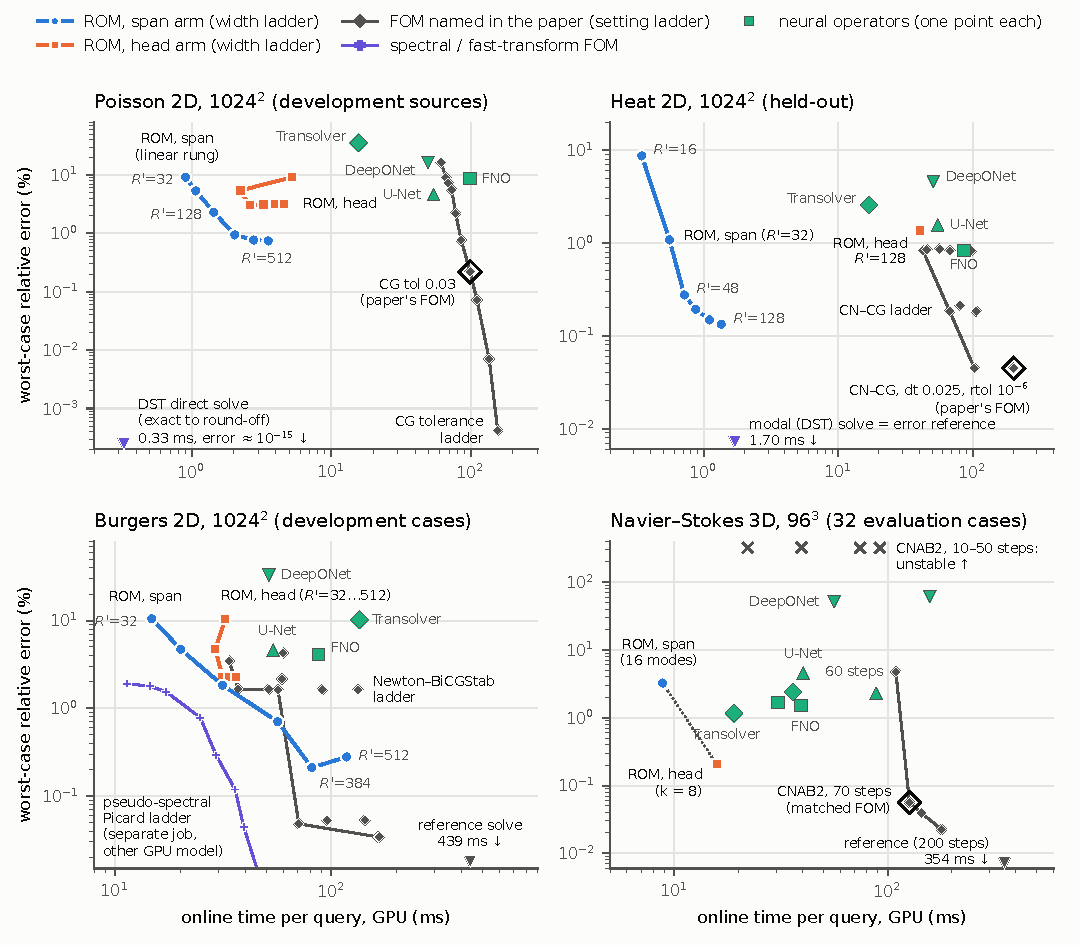
\includegraphics[width=0.8\linewidth]{figs/F1_tunability.pdf}
\caption{Error against cost. Worst-case relative error against median
online GPU time per query on four problems of the original benchmark set.
Blue: span along its width ladder $R'$; orange: head; grey diamonds: the
named full-order solver along its own ladder; violet: transform or
pseudo-spectral solvers; green: neural operators (one point per trained
model). Poisson 2D and Burgers 2D panels are development cohorts at
$1024^2$ (held-out errors are higher), heat 2D at $1024^2$, original
Navier--Stokes at $96^3$. Points come from more than one job (5--20\,\%
cross-job timing differences). On these problems the transform and
pseudo-spectral solvers are faster at equal error, which the figure
shows.}
\label{fig:tunability}
\end{figure}

\begin{figure}[htbp]
\centering
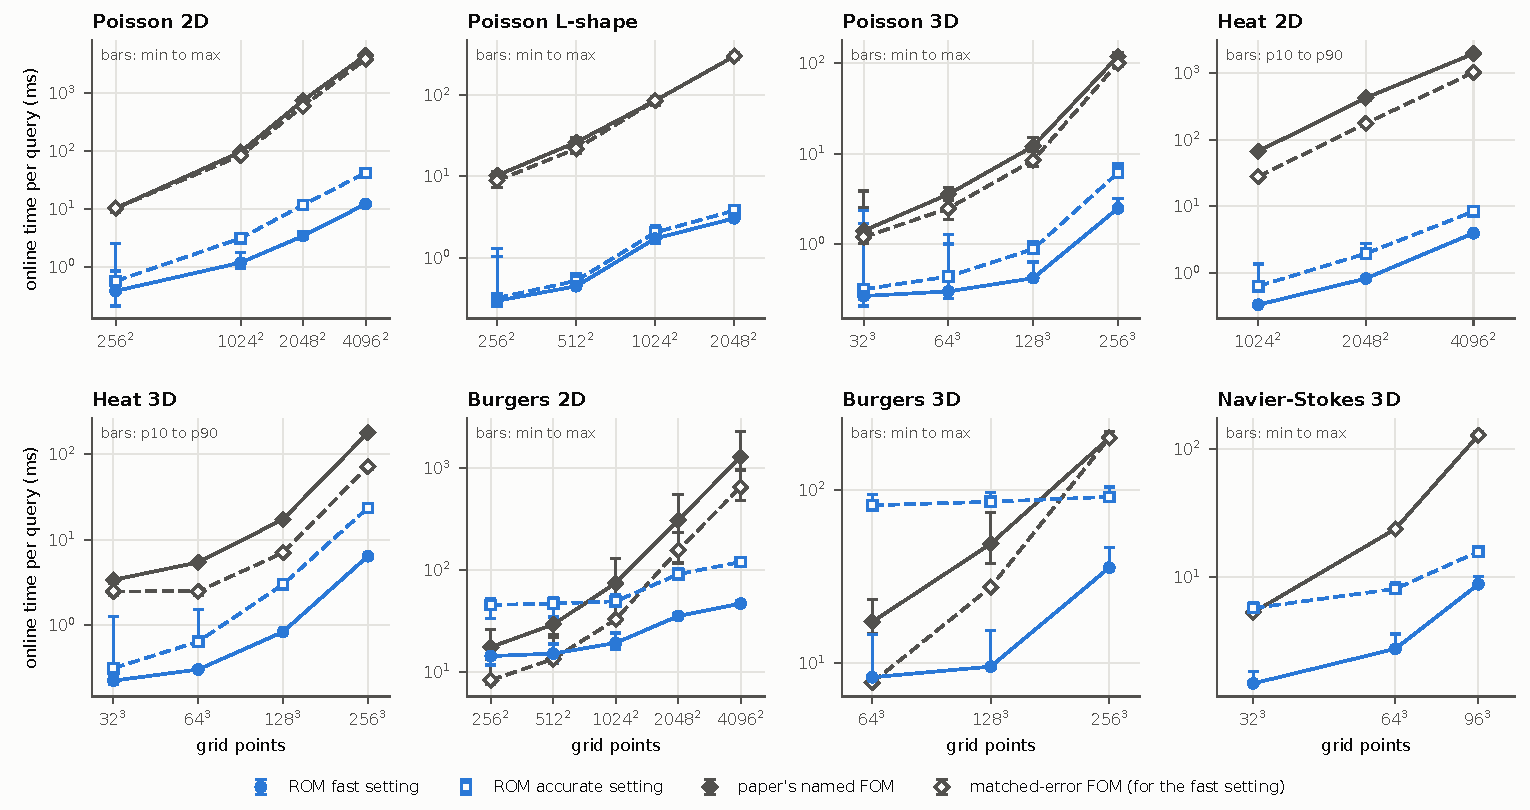
\includegraphics[width=\linewidth]{figs/F2_cost_vs_mesh.pdf}
\caption{Cost against mesh. Median online time per query against the
number of grid points for the problems of Tables~\ref{tab:headline}
and~\ref{tab:boxes}. Blue solid: fast setting; blue dashed: accurate;
grey solid: the submission's named solver; grey dashed: the fast
setting's matched solver. Bars: minimum to maximum over stored repeats
(heat: 10th to 90th percentile).}
\label{fig:costmesh}
\end{figure}

\begin{figure}[htbp]
\centering
\rev{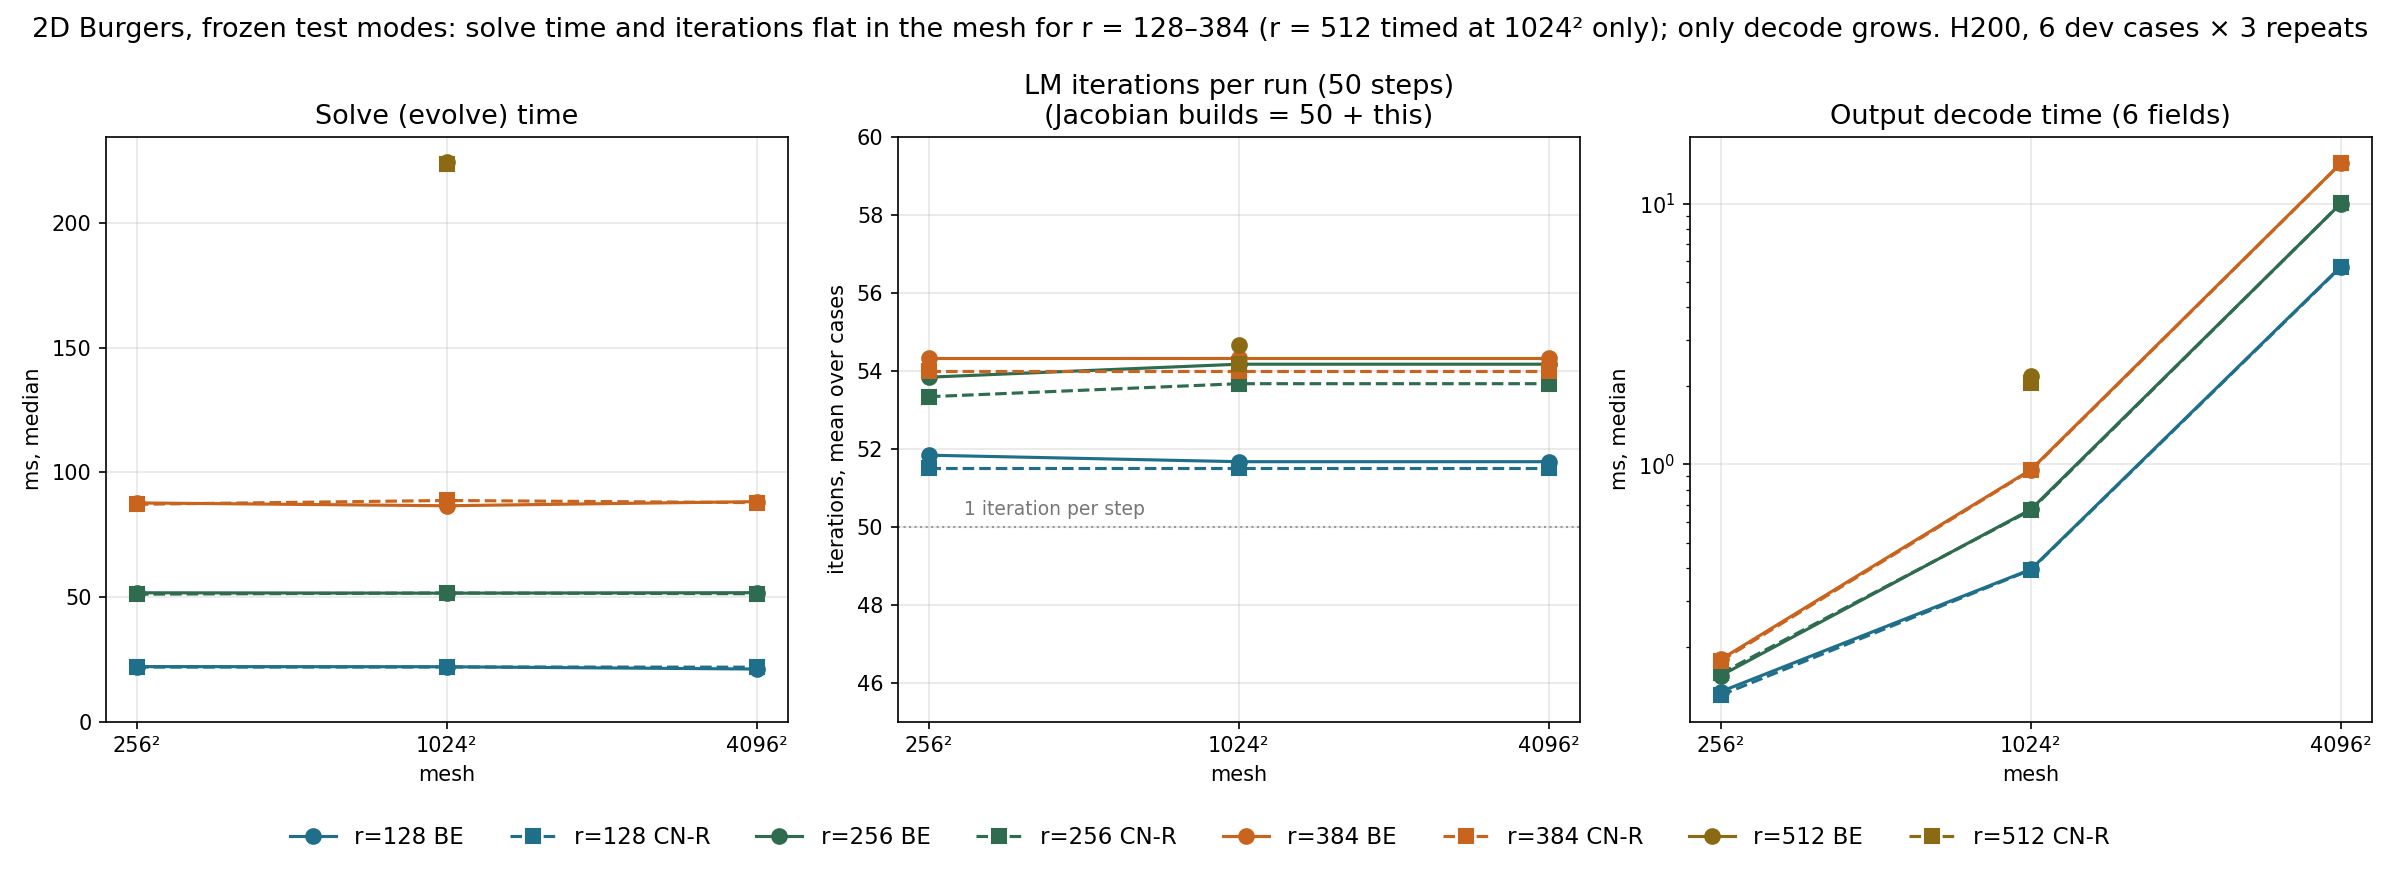
\includegraphics[width=\linewidth]{figs/F2b_mesh_flat_burgers2d.png}}
\caption{\rev{The reduced evolution does not grow with the mesh. Burgers 2D,
the submission's frozen bank with a later off-mesh solver variant (frozen sine
tests), bank widths $r=128$--$384$ (two time integrators each), 50 time steps
per query, six development cases with three repeats on one H200 GPU. Left: median solve time is
unchanged from $256^2$ to $4096^2$ ($22.1/22.0/21.1$\,ms at $r=128$,
$51.7/51.6/51.8$\,ms at $r=256$, $87.8/86.6/88.3$\,ms at $r=384$). Middle:
Levenberg--Marquardt iterations per query are the same at every mesh. Right:
only writing the six output fields grows with the mesh ($0.13$ to $5.7$\,ms at
$r=128$). At width 384 with backward Euler the worst-case error changes by
$0.014$ percentage points across these meshes. This is scaling evidence, not a
speed claim: in the same study this variant was slower than the best full
solver at matched accuracy at $4096^2$ ($0.05$--$0.71\times$), with the gap
closing as the mesh grows. The width-512 bank was timed at $1024^2$ only.}}
\label{fig:meshflat}
\end{figure}

\begin{figure}[htbp]
\centering
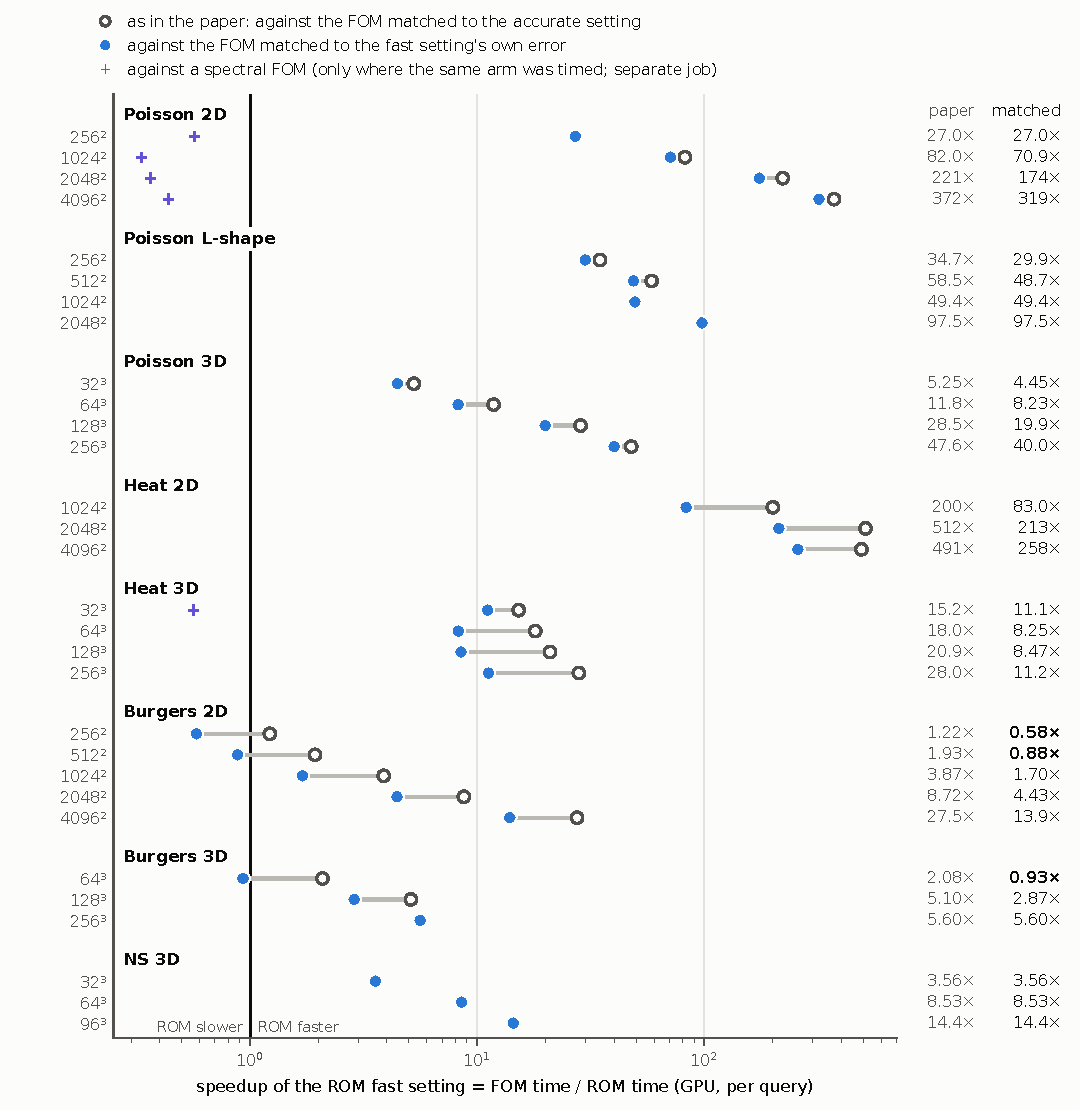
\includegraphics[width=0.7\linewidth]{figs/F3_matched_speedup.pdf}
\caption{Matched speedups. For the 30 cells of the submission's Table~1:
speedup of the fast setting over the submission's named solver (filled)
and over the rung of the same solver matched to its own error (open).
Violet: transform or pseudo-spectral solvers where measured. Three cells
fall below 1 (Burgers 2D $256^2$ and $512^2$, Burgers 3D $64^3$). The
Navier--Stokes cells are against CNAB2 on the same mesh; against a solver
free to coarsen its mesh see \S\ref{sec:results:fom}.}
\label{fig:matched}
\end{figure}

\begin{figure}[htbp]
\centering
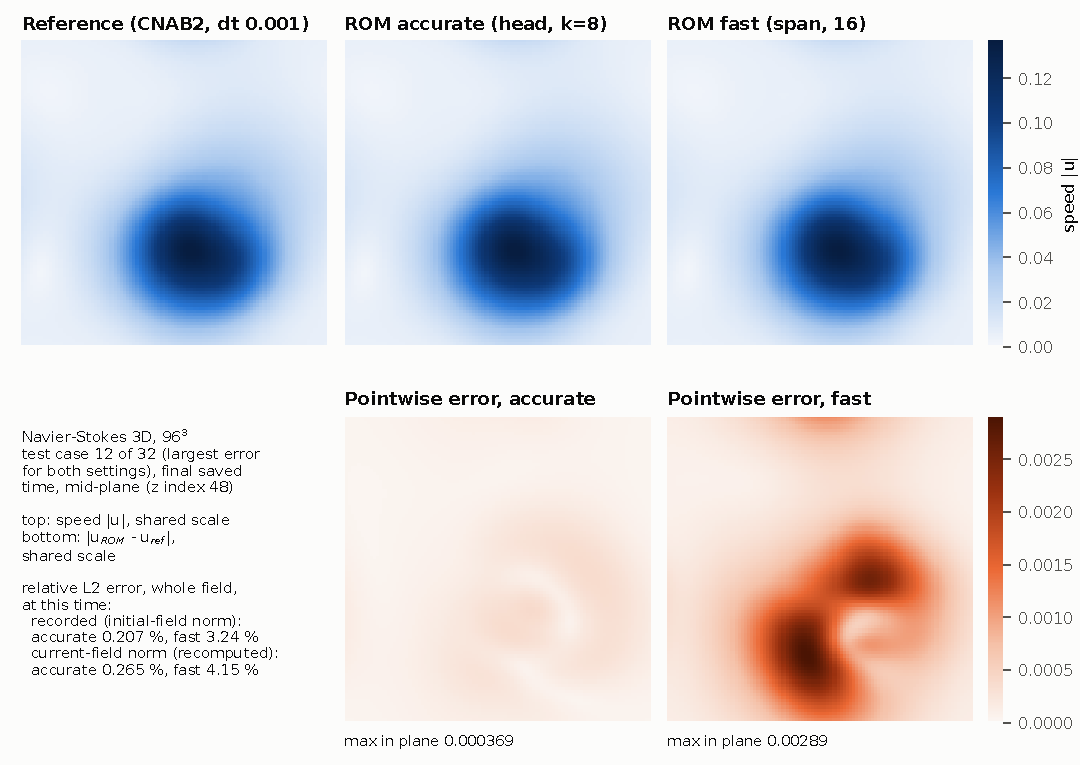
\includegraphics[width=0.8\linewidth]{figs/F4a_fields_ns3d_96.pdf}
\caption{Solution field and error map, original Navier--Stokes family at
$96^3$: speed $|u|$ on the mid-plane at $t=0.2$ for the test case with the
largest error. Top: reference, head ($k=8$), span ($R'=16$); bottom:
$|u_{\mathrm{ROM}}-u_{\mathrm{ref}}|$, one shared scale.}
\label{fig:fields-ns}
\end{figure}

\begin{figure}[htbp]
\centering
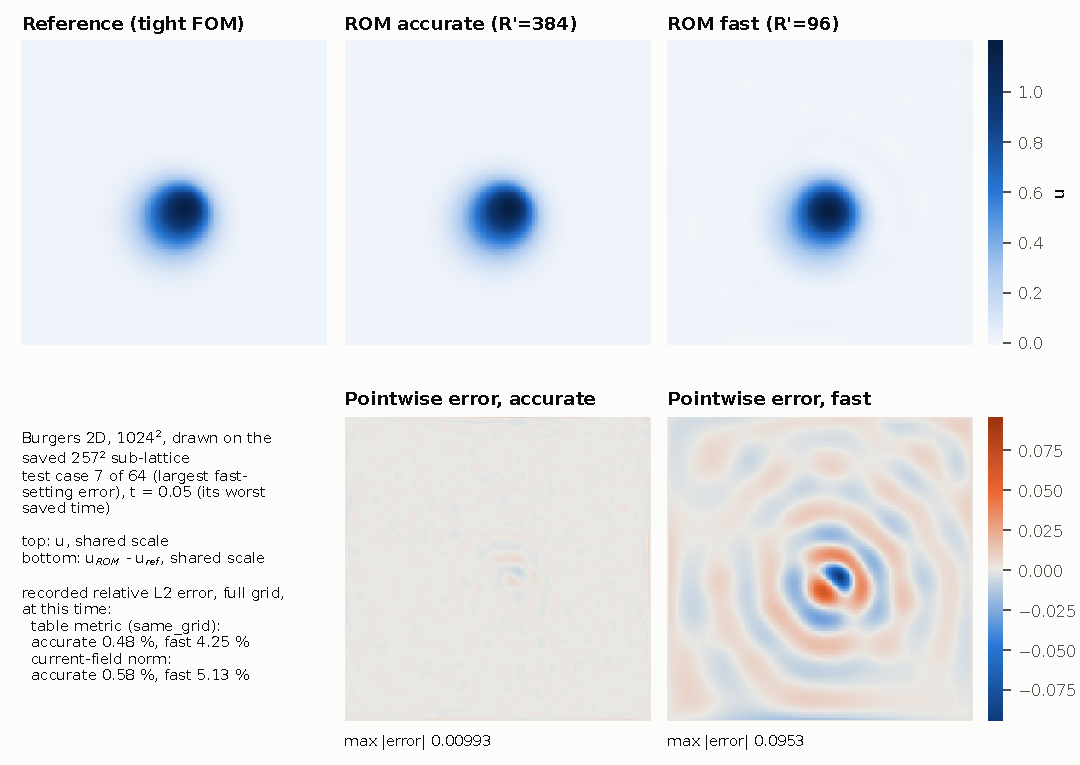
\includegraphics[width=0.8\linewidth]{figs/F4b_fields_burgers2d_1024.pdf}
\caption{Solution field and error map, Burgers 2D at $1024^2$, $t=0.05$,
held-out case 7 (the fast setting's worst case), on the stored $257^2$
restriction. Top: reference, accurate ($R'=384$), fast ($R'=96$);
bottom: signed pointwise error.}
\label{fig:fields-b2d}
\end{figure}

\begin{figure}[htbp]
\centering
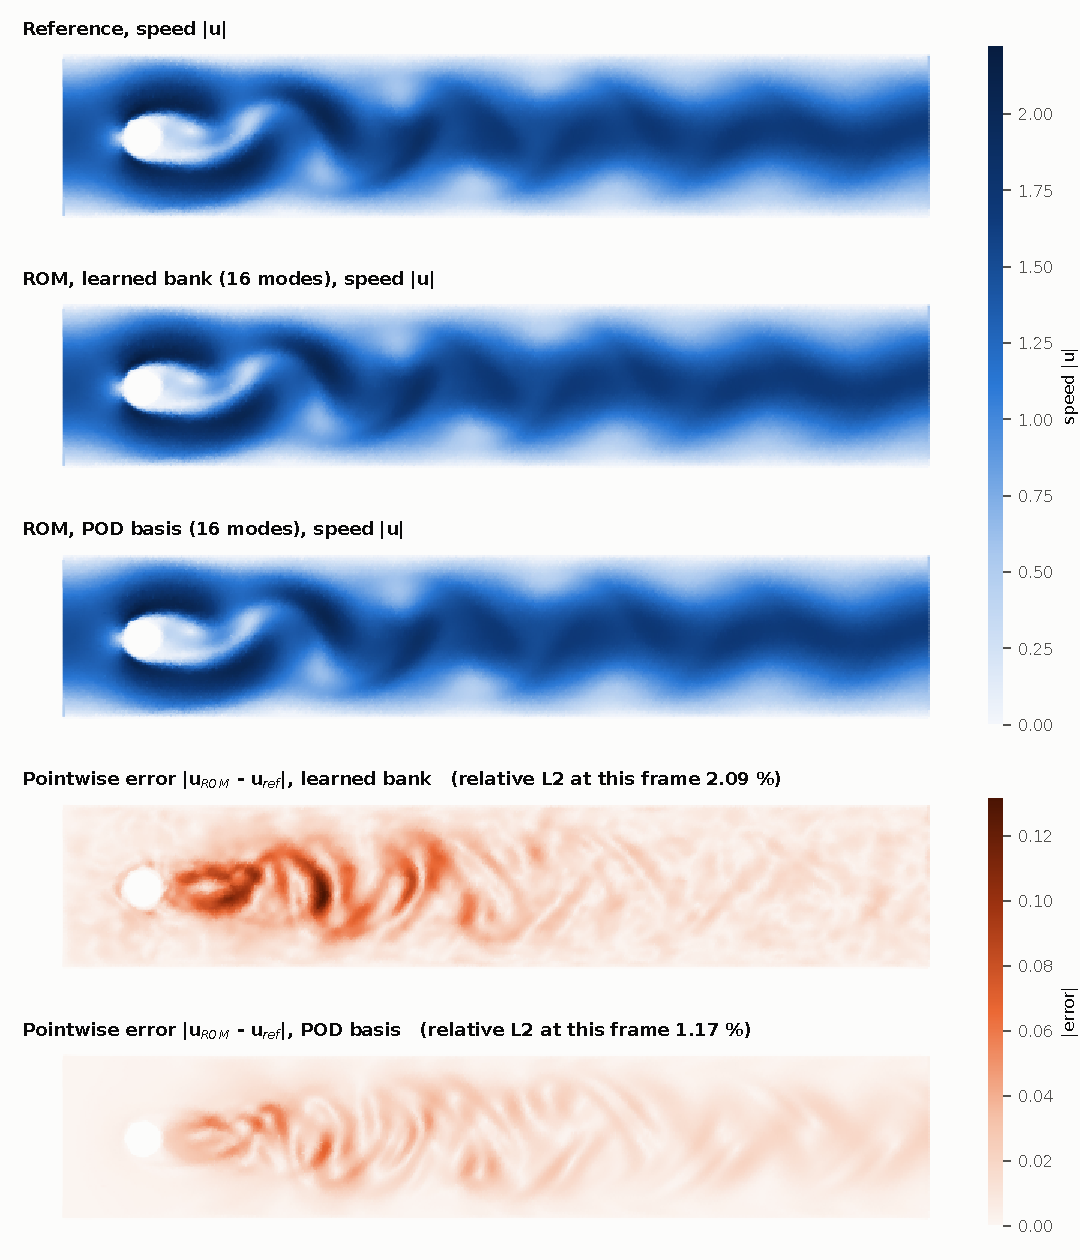
\includegraphics[width=\linewidth]{figs/F4c_fields_cylinder_re95.pdf}
\caption{Solution field and error map, cylinder flow, development
Reynolds number 95, last stored frame: reference, a width-16 bank and a
width-16 POD basis (top), velocity error magnitude (bottom). This
rendering uses the first retrained bank of an earlier campaign, which is
less accurate than POD here (2.1 against 1.2\,\% at this frame); the bank
of Table~\ref{tab:g2} matches POD within 1\,\%.}
\label{fig:fields-cyl}
\end{figure}

\begin{figure}[htbp]
\centering
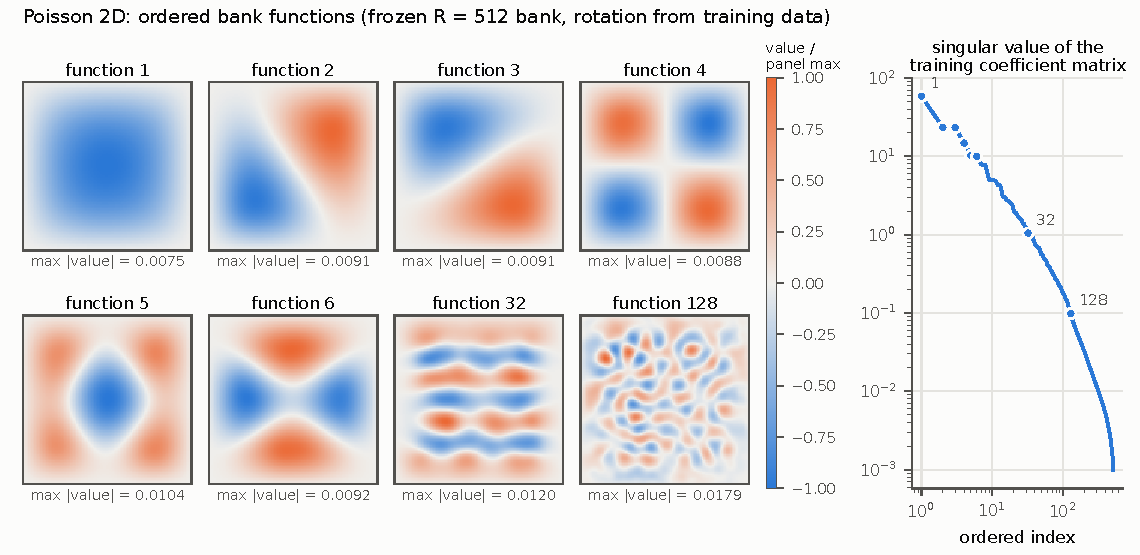
\includegraphics[width=0.85\linewidth]{figs/F5_basis_poisson2d.pdf}
\caption{Learned basis functions: ordered bank functions 1--6, 32 and 128
of the frozen $R=512$ Poisson 2D bank, each scaled by its own maximum, and
the singular values that define the ordering. Low indices are smooth and
large-scale; high indices carry fine scales.}
\label{fig:basis}
\end{figure}

\begin{figure}[htbp]
\centering
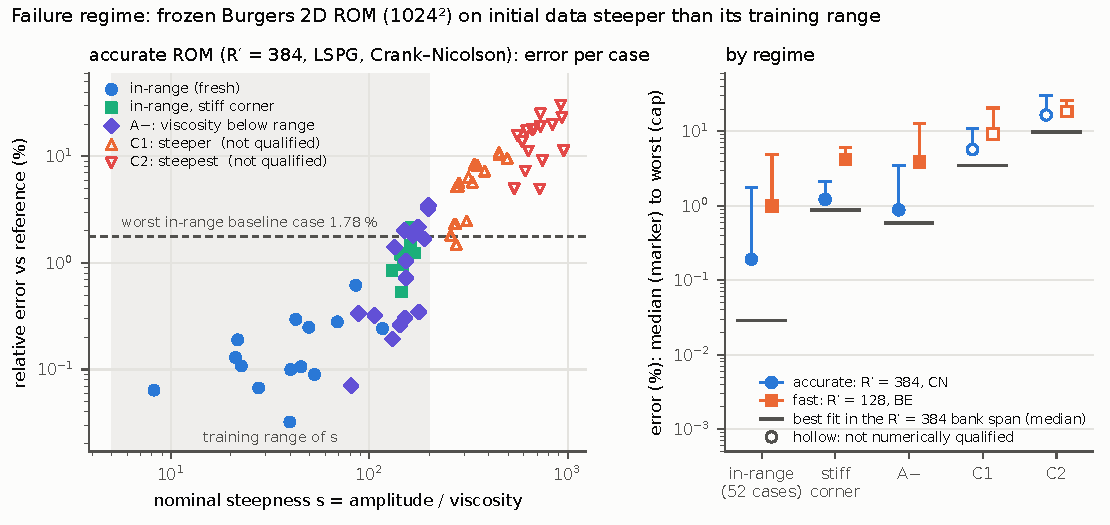
\includegraphics[width=\linewidth]{figs/F6_failure_burgers2d_steep.pdf}
\caption{Failure case: Burgers 2D at $1024^2$ on initial data steeper
than the training range (steepness $s$ = amplitude/viscosity; training
range shaded). Left: error per case of the accurate setting against $s$;
hollow markers: regimes where the solve did not pass numerical
qualification. Right: median to worst error per regime for the accurate
and fast settings; grey: best fit in the bank's span. Medians rise to
5.7\,\% and 16.6\,\% on the two steepest exploratory development regimes,
and the fit floor rises with them: the bank cannot represent these
states. Metric: maximum over saved times relative to the initial norm.}
\label{fig:failure}
\end{figure}

\begin{figure}[htbp]
\centering
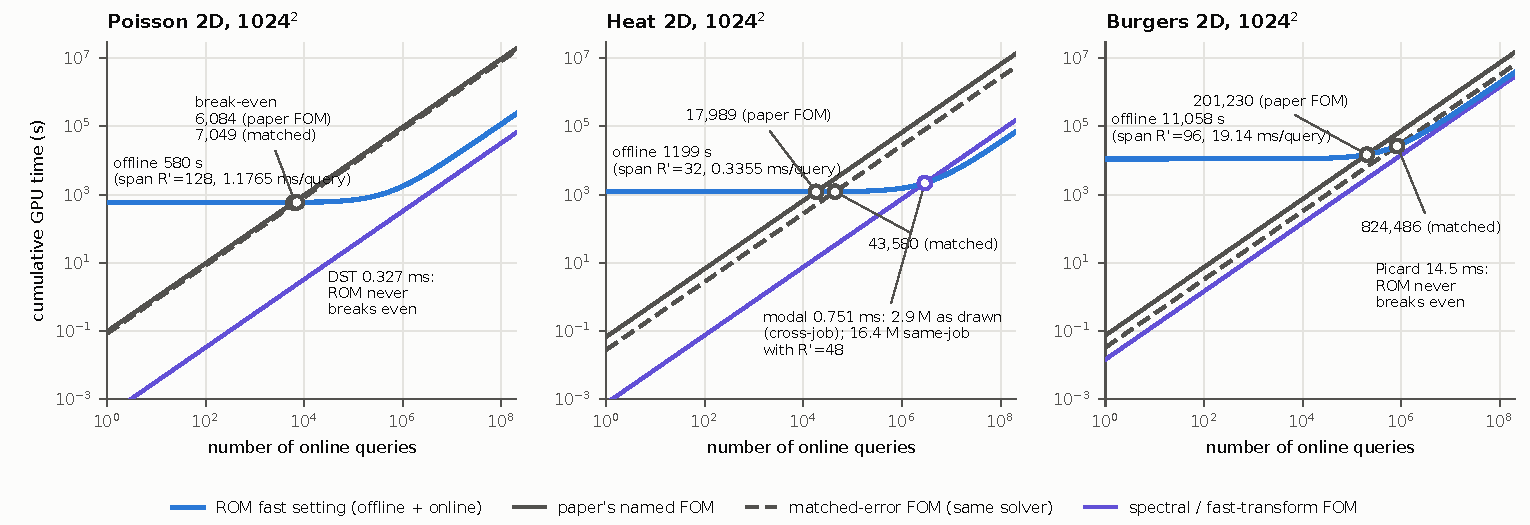
\includegraphics[width=\linewidth]{figs/F7_breakeven.pdf}
\caption{Break-even curves: cumulative GPU time against number of queries
at $1024^2$ for Poisson 2D, heat 2D and Burgers 2D. Blue: fast setting
including offline cost; grey solid: the submission's solver; grey dashed:
matched solver; violet: transform or pseudo-spectral solver (never
crossed for Poisson and Burgers at this mesh). Largest-mesh counts are in
Table~\ref{tab:breakeven}.}
\label{fig:breakeven}
\end{figure}
\end{revblock}


\end{document}
